\documentclass[pdflatex,final]{pittetd}%   If you want to use dvipdfm. The file is to be normally processed (LaTeX), and 
%                                   then the program dvipdfm applied to it. This will create the PDF file with bookmarks
%                                   and links. It will also try to convert any PS graphics included.
%\documentclass[pdftex]{pittetd}    If you want to use PDFLaTeX instead. This will create the PDF file directly.
%                                   Processing time can be longer. No PS graphics conversion will take place 
%                                   automatically.
%
%Other options: ma, ms, for Master's. 
%11pt, 10pt, font size (12pt is default). 
%final, makes pittetd's warnings (about things that might go against the Format Guidelines) 
%into error messages. 
%Option 'sectionletters' numbers the chapters with Roman numerals (I, II, etc.), sections with 
%letters (A, B), subsections with numbers (1, 2), and subsubsections with lowercase letters (a, b). 
%The four levels of the enumerate environment receive the same treatment. Within the
%text, however, cross references (\ref} produce `the whole thing,' something like I.A.1 
%instead of only 1.

% Packages included in PittETD Template
% auto use this package and check for patches
\usewithpatch{graphicx} 
% manually use these packages
\usepackage{amsmath,amsthm}%        But you can't use \usewithpatch for several packages as in this line. The search for
%                                   patches has to be then forced through:
\patch{amsmatch}
\patch{amsthm}

% Jenna's commonly used packages
\usepackage{amssymb}
\usepackage{amsmath}
%\usepackage{amsthm}
\usepackage{graphics} % for improved inclusion of graphics
%\usepackage{wrapfig} % to include figure with text wrapping around it
\usepackage{subcaption} % fit multiple graphics in one figure
%\usepackage[margin=10pt,font=small,labelfont=bf]{caption}
\usepackage{algorithm}
%\usepackage{algorithmic}
\usepackage{algpseudocode}
\usepackage{hyperref}
\usepackage{multirow}
\usepackage{listings}
\usepackage{apalike}
\usepackage{soul}
\usepackage{color}

\lstset{
  language=Python,
  basicstyle=\ttfamily,
  numbers=left,
  numberstyle=\tiny,
  numbersep=5pt,
  showstringspaces=false,
}

\def\sectionautorefname{Section}
\def\chapterautorefname{Chapter}

% Bibliography
\bibliographystyle{apalike}

\title[Correction, Validation, and Characterization of Motion in Resting-State Functional Magnetic Resonance Images of Pediatric Patients]{Correction, Validation, and Characterization of Motion in Resting-State Functional Magnetic Resonance Images of Pediatric Patients}
% The optional argument is the 
% version of the title that will appear in Acrobat Reader's Document Info dialog box.
\author{Jenna Marie Schabdach}
\degree{B. S. Electrical Engineering, Drexel University, 2016\\M. S. Electrical Engineering, Drexel University, 2016\\M. S. Biomedical Informatics, University of Pittsburgh, 2018}
\date{March 31, 2020}%             This date is the date of the thesis defense. Default is \today
\year{2020}
% pittetd will use the current year unless otherwise indicated. So this command is not necessary.
\keywords{resting-state fMRI, medical imaging, motion correction}% This list appears in the field 'Keywords' of Acrobat Reader's Document Info
%                                   dialog box, and also, optionally, after the abstract.
\subject{J Schabdach Biomedical Informatics Dissertation}%              This fills in the 'Subject' field in Acrobat Reader's Document Info dialog box.
\school[School of Medicine]{Department of Biomedical Informatics}

\begin{document}
  
%\chapterfloats%                    Un-comment this to get figures and tables numbered within chapters.
\maketitle
%
% For the committee membership page, you have to provide the names and affiliations of the members. The first one will 
% be treated by pittetd as the committee chair (thesis/dissertation advisor).
\committeemember{Dr. Douglas Landsittal, Department of Biomedical Informatics}
%\coadvisor{Second advisor, Dept. Aff.}%         This is used if there are two advisors.
\committeemember{Dr. Ashok Panigrahy, Department of Biomedical Informatics}
\committeemember{Dr. Gregory Cooper, Department of Biomedical Informatics}
\committeemember{Dr. Rafael Ceschin, Department of Pediatric Radiology, Children's Hospital of Pittsburgh of UPMC}

% etc., as many as needed. For master's theses, the committee may be omitted, naming only the advisor.
\school{School of Medicine}
\makecommittee

\copyrightpage                     

\begin{abstract}
Approximately 1.35 million children are diagnoses with a congenital heart defect (CHD) annually. As the process of diagnosing and treating CHD has improved, the expected lifespan of CHD patients has increased: at least 12 to 34 million adults worldwide have CHD. A larger population living with CHD means that clinicials are learning more about conditions which CHD patients are at increased risk of getting. Some of these conditions affect the patient's neurodevelopment and neurocognitive status. Diagnosis of the neurocognitive conditions is performed using surveys, but examining the structure and function of the brain could offer more objective diagnoses. 

One tool useful for examining a patient's brain is magnetic resonance imaging (MRI). Resting state functional MRI (rs-fMRI) in particular can be used to reveal information about the neuronal networks in the patient's brain. Unfortunately, rs-fMRIs are highly susceptible to motion. Clinical and behavioral techniques can help patients move less during a rs-fMRI scan, though they do not guarantee motion-free images. Various sensors can be used to monitor and correct for motion during the scan, but these sensors are useless when it comes to recovering previously acquired rs-fMRIs corrupted by motion.

We devised a novel approach to volume registration, which is the first step in motion correction. We compare it to traditional volume registration in the context of a complete motion correction pipeline. The registration techniques and pipeline were applied to neurological rs-fMRIs of fetal, neonatal, preadolescent, and adult patients with CHD as well as several phantom images. We identified different motion patterns specific to different demographic groups, and discovered relationships between certain motion patterns and clinical outcomes associated with CHD and different neurodevelopmental conditions.
\end{abstract}

% If you say \begin{abstract}[Keywords:] instead of the simple \begin{abstract}, a list of the keywords is appended.
% The list comes from the \keywords command above.
% The starred version \begin{abstract*} typesets the word `ABSTRACT' on the top of the page
\tableofcontents
\listoftables                     
\listoffigures                     

\preface

\section{DEDICATION}
To the patients being treated in children's hospitals all over the world, their families, and the people working to help them.         

\clearpage

\section{ACKNOWLEDGEMENTS}

This project would not have been possible without the assistance and support of many people. First, to my committee members: Dr. Doug Landsittal, Dr. Ashok Panigrahy, Dr. Greg Cooper, and Dr. Rafael Ceschin. Your guidance and suggestions were truly invaluable. Second, to the members of PIRC, especially: Julia Wallace, Vince Lee, and Nancy Beluk, for helping wrangle the data and answering questions about behavioral techniques used during pediatric scans; Dr. Vincent Schmithorst, for the many conversations about the intricacies of MR physics; Billy Reynolds, for the fetal data and for pulling the occasional perfect figure seemingly out of thin air; and Samuel Cho, for helping me develop the data simulation and aptly naming it ``SPECTr''. Third, this document would not be the same without the Writing Accountability Groups organized and run by Dr. Moriah Kirdy through the Pitt Writing Center. Moriah's dedication and organization is (thankfully) contagious. 

A successful dissertation is only partly made up of the research and writing. The rest is managing people, places, and paperwork. Many thanks to Toni Porterfield and Tami Robinson for helping me keep my administrative ducks in a row and to Barbara Karnbauer for helping coordinate schedules. 

Of course, I would like to thank my friends and family. Ryan, for keeping me grounded, and for rock climbing, burritos, and ice cream. My friends in and around Philadelphia and Pittsburgh, for the laughs, game sessions, and more rock climbing. Mom and Dad, thanks for supporting me the way you always do. Jonathan and David, I'm over the moon you were able to make my defense. 

Finally, special thanks to everyone involved with Extra Life, a charity that raises money for kids being helped by Children's Miracle Network Hospitals. As promised, here is the shout out to those who donated to my page, especially to Leo Chan, Elliot Guiso, Bonnie Young, John Maloney, Justine White, and Mike West.

% This is the text of the preface, with acknowledgments, dedication, etc. It is optional, and you create, as shown, by 
% just saying \preface and starting the preface's actual text. Note that 'foreword' is no longer acceptable as title
% for this preliminary.
%
%Conventions, such as notation (nomenclature) and abbreviations, don't receive their own preliminary page. They can be included as an appendix, or as part of the introduction.


% Add in chapters here
\chapter{Introduction}

Resting-state functional magnetic resonance imaging (rs-fMRI) measures the blood oxygen level dependent signal in an organ or organ system. This property makes rs-fMRI an invaluable tool for evaluating a patient's neurodevelopmental status or examining functional networks in his brain. To gather enough data to fully evaluate these networks, a series of image volumes must be acquired over a period of several minutes. In a standard rs-fMRI (?), one new image volume is obtained approximately once every two to three seconds. To gather high quality data on such a short timescale, the rs-fMRI suffers from two major limitations: rs-fMR images have low physical resolution and are highly susceptible to motion. The first limitation can be addressed by obtaining an MR image with high physical resolution and registering the rs-fMRI to this structural image, but the second limitation requires the patient to remain as still as possible for the entire duration of the scan. This task is particularly difficult for populations of certain ages or populations who suffer from conditions that affect neurodevelopment. As a result, it is common for an image from a member of one of these populations to contain too much motion to be used in clinical or research applications.

Various behavioral and XX protocols have been developed in an attempt to prevent patients from moving during MRI scans, though many of these protocols are not applicable to younger populations. In particular, a neonate or fetus cannot understand instructions to stay still, and young children who can understand the command have difficulty following it. Sedation is not advisable for these young populations. After a rs-fMR image is acquired, however, it is possible to reduce the positional effects of motion in the image sequence.

Limitations of traditional methods

DAG-based registration

Apply DAG-based registration to neonates and preadolesents

Real goal is to develop a method of registering fetal brain and placental images so that we can further examine the relationship between placental oxygen levels and fetal brain development. Longitudinally, this technique can be used to determine how placental oxygen flow and fetal brain development impact a patient over the course of his or her life. Once the relationship between the placenta and fetal brain development is better understood, we can determine a set of neuroprotective interventions to employ for at-risk patients before they are born.
\chapter{rs-fMRIs and Patient Motion}
\label{ch:mri}

This chapter discusses rs-fMRIs and how they are affected by patient motion. Specific topics include the structure of rs-fMRIs, sources of motion, quantifying motion, and a review of current methods for preventing and managing motion in rs-fMRIs.

\section{Structure of an rs-fMRI}

rs-fMRIs are discrete representations of continuous data. A new image volume of the patient's brain is acquired every two to three seconds. The image volume is composed of a three-dimensional version of a pixels called a voxels (volume element). Each voxel encompasses a small volume of physical space. The amount of space represented by a voxel is its physical resolution. The ``distance'' between each image volume is a period of about two to three seconds. This distance is the temporal resolution of the image sequence.

The concept of a 4D rs-fMR image is illustrated in two different ways in Figure \ref{ch2:fig:rsfmri-views}. The first representation is an ordered list of 3D image volumes where each voxel contains a single numeric value. The second representation is a single 3D image volume, where the value of each voxel is a temporal signal.

An rs-fMRI is considered to have a relatively low spatial resolution but high temporal resolution. The physical size of a single voxel seems small at about 4 mm$^3$, but this resolution is not granular enough to capture details about activity within small structures of the brain. The activity information recorded during an rs-fMRI must be combined with the detailed anatomic information from a structural MRI to know precisely which areas of the brain are active at each point in time. A structural MRI volume takes much longer to acquire than an rs-fMRI volume, which can be obtained every two to three seconds. Unfortunately, the patient's position and neural activity can change faster than the image volume can be acquired. As a result, a temporal resolution of two to three seconds is not fast enough to actively compensate for sources of noise which confound the BOLD signal. 

\begin{figure}
\centering
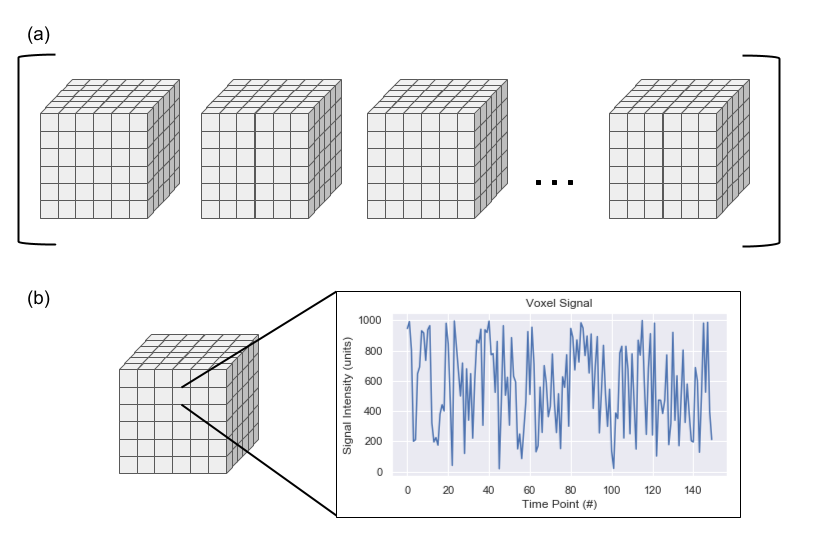
\includegraphics[width=1.0\textwidth]{2/rsfMRI-views.png}
\caption{A rs-fMRI can be thought of (a) as a sequence of image volumes or (b) as a single volume where each voxel contains a temporal signal rather than a single numeric value.}
\label{ch2:fig:rsfmri-views}
\end{figure}

\clearpage

\section{Factors Impacting rs-fMRIs}

The BOLD signal present inside a patient's brain is not recorded with complete accuracy by an MRI scanner. Even if the same patient exhibited precisely the same BOLD signal during two different scans, the recorded image sequences would vary slightly. Several factors impact the image sequence viewed by a radiologist, and we give an overview of them in Figure \ref{ch2:fig:signal-filters}. 

The first factor in Figure \ref{ch2:fig:signal-filters} is the patient's physiology. An rs-fMRI is not sensitive enough to detect brain activity on a neuronal level. Instead, it measures the changes in the amounts of deoxygenated hemoglobin in the brain. The deoxygenated hemoglobin quantities are highly correlated with brain activity because active areas of the brain use more oxygen than inactive areas, but the BOLD signal is still only an approximation of brain activity.

The second factor in Figure \ref{ch2:fig:signal-filters} represents the changes to the signal that occur due to patient motion.
During every medical imaging scan, the patient will naturally perform small, automatic movements due to regular bodily functions. Minuscule movements caused by cardiac activity may disrupt scans with high spatial resolution or with high sensitivity to the movement of blood molecules. More significant movements caused by respiration result in motion artifacts in images of the thoracic and abdominal cavities. 

\begin{figure}
\centering
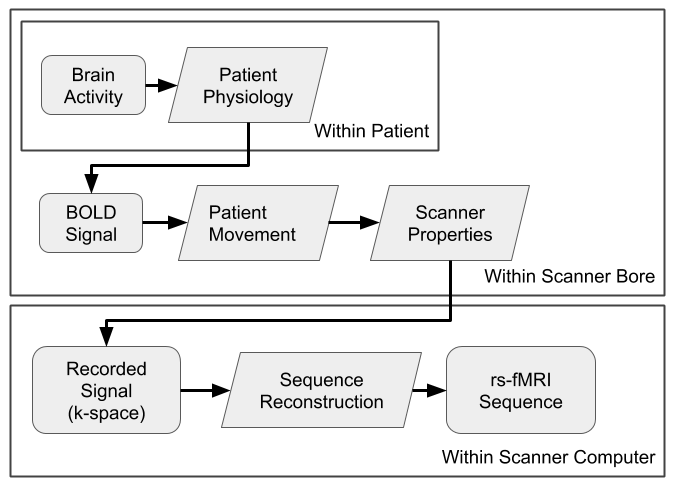
\includegraphics[width=.72\textwidth]{2/rsfMRI-signal-filters.png}
\caption{The patient's brain activity is affected by several factors before an MRI scanner produces a visually interpretable image sequence. (The rounded rectangles represent the signal at different stages of recording while the rhombuses represent the primary factors.)}
\label{ch2:fig:signal-filters}
\vspace{-30pt}
\end{figure}

Other motions occur on a larger and more conscious scale. It is important to note that different populations may exhibit more of certain macro-motions than others. The patient may fidget or shift his gaze when he becomes bored in the scanner. If the patient falls asleep during a scan, there may be slight movement as the body relaxes and re-tenses if the patient wakes. Certain MRI protocols are known to produce loud sounds: during one of these protocols, the patient may become surprised and react by jumping. Additionally, claustrophobic patients or patients who feel secure around specific people that are not allowed in the scanner room may become agitated. 

Both the small-scale, automatic motions and the large-scale, reflexive motions corrupt the BOLD signal. These effects of patient motion will be discussed in-depth in the next~section.

The third factor in Figure \ref{ch2:fig:signal-filters} is the unique properties of the scanner. The acquired image sequence will vary slightly even in machines made by the same company because each scanner has a unique primary magnetic field, $B_0$. The $B_0$ inhomogeneities can be measured using a primary field map. These field maps can be used to correct signals displaced by the $B_0$ field, though they cannot be used to recover signals corrupted by the field.

The final factor is also related to the properties of the MRI scanner. The image sequence produced by a scanner is dependent on the scanner vendor. Different vendors use different proprietary algorithms to convert the signal recorded by the scanner in k-space into a visually interpretable image sequence. Between the $B_0$ inhomogeneities and the scanner vendor differences, the differences in the scanners used to acquire the sequences must be resolved before images from different scanners can be compared.

\clearpage

\section{Effects of Patient Motion}

Due to their low spatial and high temporal resolutions, rs-fMRIs are highly susceptible to all types of motion outlined in the previous section. In general, motion affects an acquired image sequence in three ways. The first and most obvious effect is the position of the patient changes throughout the sequence. The second effect is due to the way changes in the patient's position affect the signal recorded by the scanner. The third effect is related to the magnetic fields in patient tissue and changes in their orientation within $B_0$. These three effects will hereafter be referred to as the positional effect, the spin history effect, and the susceptibility effect of motion.

\subsection{The Positional Effects of Motion}

The technique used for analyzing neuronal network activity rs-fMRIs, called functional connectivity analysis, assumes that the contents of one voxel at every time point during the sequence all contain signals from a single point in the brain. This assumption is vital in the process of inferring networks of neuronal activity. 

While rs-fMRIs have a spatial resolution on the order of millimeters, neuronal activity occurs on the spatial resolution of microns. As a result, each voxel in an rs-fMRI volume contains information from a number of neurons. The smallest movement of the patient can alter the voxel to which a cluster of neurons contributes. These seemingly insignificant changes can alter the position of the patient enough to cause the voxels to record signals from different brain regions or even tissue types. This change in voxel location within the brain violates the assumption that single voxels record from the same location within the brain for the duration of the sequence.

\subsection{The Spin History Effects of Motion}

In addition to changing the recorded position of the patient, motion impacts the established spin gradients, which introduces artifacts into the image sequence.

During an ideal MRI scan, the patient is sitting in the scanner and all molecules become aligned with the primary magnetic field $B_0$ in a relaxed state. Then, a radiofrequency (RF) pulse is applied to the field. The purpose of the pulse is to excite the molecules in a particular volume of physical space change their orientation to match the induced perpendicular field. When the pulse ends, the molecules precess back to their orientation in $B_0$. As they do, their small magnetic fields induce electric currents on the RF coil. The currents are recorded by the scanner as signals in frequency space. The volume of the space intended to be excited is known, and the signal produced by the induced electric current is used in conjunction to reconstruct the image in voxel space.

However, when the patient moves, the volume of space which was thought to be excited is not actually excited: some other volume of space, which may or may not overlap with the intended volume of space, is excited instead. Because the MRI scanner has no way to know this assumption is not correct, it does not know that not all of the molecules in its intended area are relaxed and correctly aligned to the $B_0$ field at the end of the RF pulse. The scanner proceeds with the next RF pulse, which excites a new set of ``relaxed molecules'', some of which are still excited from the previous pulse. As a result, the signals produced in the second RF pulse are different than they should be. Signals that are artificially decreased result in dark shadows within motion affected volumes of the sequence, while signals that are artificially increased result in bright spots.

The previous few paragraphs in this section describe how motion disrupts the magnetic spin gradients present in the patient during an rs-fMRI scan. The spin gradients need time to recover to the correct magnetic field orientation, and up to eight to ten seconds may pass before the recovery is complete \cite{Power2014}. While the spin gradients are reorienting, the recorded BOLD signal will vary more than expected between temporally neighboring volumes. These variations are more difficult to quantify than the positional effects of motion.

The nature of the $B_0$ field in an MRI scanner can be recorded using a field map. Acquiring a field map while the patient is in the scanner records information about how the patient interacts with the $B_0$ field. These field maps of the patient in the scanner can be used to perform distortion correction on the acquired sequence. A study of the effects of distortion correction on rs-fMRIs of 40 healthy subjects suggested that distortion correction using field maps can increase the functional connectivity in rs-fMRIs \cite{Togo2017}.

\subsection{The Susceptibility Effects of Motion}

The susceptibility of a material describes how the material will behave when placed in a magnetic field. Most materials are either paramagnetic or diamagnetic. Paramagnetic materials are attracted to and align with magnetic fields. Diamagnetic have the opposite interaction: they are repelled from and become anti-aligned with magnetic fields. Additionally, paramagnetic materials contribute to the magnetic field, while diamagnetic materials detract from it. 

Both types of materials cause distortions in the magnetic field. These distortions are prominent in stronger magnetic fields and at the interface of two different material types. In MRI scanners, the differences in susceptibility between soft tissue and bone or between soft tissue and air can produce artifacts in the acquired sequence. These artifacts are amplified when the patient moves. When the patient moves, the interfaces between tissues and air distort the $B_0$ field. The distortions in the $B_0$ field change the electromagnetic signal recorded by the scanner and lead to spurious correlations during the analysis of the rs-fMRI sequence.

Susceptibility artifacts can be reduced using susceptibility maps. Susceptibility maps are short acquisitions that use multiple echo periods to detect small changes in the location of susceptibility interfaces in an MRI sequence. They are not part of most rs-fRMI acquisition protocols.

\section{Measuring Motion}

Even though we described three effects of motion on rs-fMRIs in the previous section, these effects impact the sequence in two areas: the position of the patient and spurious signal correlations throughout the sequence.

\subsection{Measuring Motion: Patient Position} 

The effect of motion on patient position is measured as the difference in the positions of subsequent image volumes. The difference in position is determined using metrics calculated by performing rigid volume registration on the two volumes. 
In rigid volume registration, one volume is chosen as the reference volume and the other is the moving volume. The reference volume remains stationary while the moving volume is translated and rotated in three-dimensional space on top of it. The registration is complete when the position of the patient in the moving volume matches the position in the reference volume. 

The moving volume can undergo linear or nonlinear transformations. Linear transformations include translation, rotation, and affine transformations along all three spatial dimensions as well as a scaling transformation. These transformations move the image volume as a whole: all voxels in the moving image remain in the same location relative to their neighbors. On the other hand, nonlinear transformations can warp the contents of the moving volume so that it better matches the contents of the reference volume. Nonlinear transformations are more complex than linear transformation. They involve additional image processing steps such as smoothing and voxel interpolation.

\begin{figure}
\centering
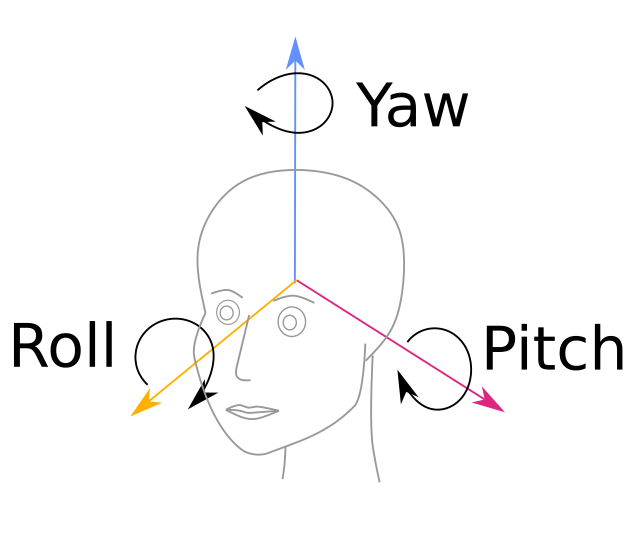
\includegraphics[width=.5\textwidth]{2/pitch_roll_yaw.png}
\caption{The pitch, roll, and yaw rotations describe rotations or an object about three orthogonal axes whose origin is in the object's center of mass.}
\label{fig:pry}
\end{figure} 

Even in cases when nonlinear transformations are used, the registration process begins with the translation and rotation transformations. The three translation and three rotation parameters used to achieve the best alignment are used to calculate the positional change between the image volumes. The positional change between temporally neighboring volumes is called the framewise displacement (FD).  

Several researchers have proposed slightly different methods for calculating the FD. Power et al., Jenkinson et al., and Dosenbach et al. each propose a slightly different method for calculating the FD \cite{Power2012} \cite{Jenkinson2002} \cite{Dosenbach2017}. All three FD calculations produce correlated metrics: the FD metric proposed by Power et al. produces measurements approximately twice as large as the metric proposed by Jenkinson et al., and Dosenbach et al. reported a high correlation between their FD and Power’s FD \cite{Yan2013a} \cite{Dosenbach2017}. 

In the remainder of this document, the abbreviation FD refers to Power et al.'s version of the FD metric, which is calculated as:

\begin{equation}
FD(J_i) = | \Delta d_{ix} | + | \Delta d_{iy} | + | \Delta d_{iz} | \\ + | \Delta \alpha_i | + | \Delta \beta_i | + | \Delta \gamma_i |
\end{equation}

\noindent where $J_i$ is the image volume $i$, $| \Delta d_{i *} |$ are the magnitude of change in position along the $x$, $y$, and $z$ axes between volumes $i$ and $i-1$, and $| \Delta \alpha_i |$, $| \Delta \beta_i |$, and $| \Delta \gamma_i |$ are the magnitude of change in pitch, roll, and yaw between volumes $i$ and $i-1$, respectively. A diagram outlining how pitch, roll, and yaw relate to the human head can be seen in Figure \ref{fig:pry}.

\subsection{Measuring Motion: Spurious Signal Correlations}

Both the spin history and susceptibility effects of motion contribute to alterations in the signal recorded and reconstructed by the MRI scanner. Without $B_0$ field maps and susceptibility maps, it is difficult to separate the impact of each of these factors on the recorded signal. We assume at this point that both the spin history and the susceptibility effects contribute equally to changes in the recorded signal intensity.

One popular metric to measure changes in the recorded signal due to patient motion was developed by Smyser et al. in 2010. Their metric is called DVARS, which measures the temporal \textbf{d}erivative of the root mean squared \textbf{var}iance over the voxels between two volumes \cite{Smyser2010}. Power et al. explain the steps to calculate DVARS in a separate study \cite{Power2012}. The DVARS value is calculated in two steps. The first step uses backward differences to approximate the derivative of the BOLD signal change between volumes $J_i$ and $J_{i-1}$ at every point $\vec{x}$ contained in both image volumes:

\begin{equation}
\frac{\partial}{\partial t} J_i(\vec{x}) \approx J_i(\vec{x}) - J_{i-1}(\vec{x}).
\end{equation}

The second step calculates the root mean square of the approximated derivatives for all $N$ points $\vec{x}$:

\begin{equation}
DVARS(J_i) = \sqrt{ \frac{1}{N} \sum_{\vec{x} \in J_i, J_{i-1}} \left( \frac{\partial}{\partial t} J_i(\vec{x}) \right)^2 }.
\end{equation}

DVARs measures the change in BOLD signal intensity, which is highly related to motion-induced spin gradient changes. 

\subsection{Acceptable Motion Quantities}

Even though the effects of motion on the patient position and the recorded signal can be measured, we still need gold standard criteria to determine whether an image containing motion can be used. Patients move slightly due to breathing and cardiac function, and the BOLD signal naturally fluctuates over time. Some motion is expected; however, we need to know how much motion can be present in the image before it is considered to be corrupted by it. Power et al. established thresholds for FD and DVARS to determine the usability of a pair of images:
\begin{itemize}
\item FD less than or equal to 0.2 mm from the previous volume, and
\item DVARS less than or equal to 25 units on a normalized scale of [0, 1000] signal units \cite{Power2014}
\end{itemize}

\noindent Image volumes that meet these criteria are considered to be low-motion.

The minimum duration of low-motion data is highly debated. van Dijk et al. established that approximately five minutes of low-motion data is sufficient for use in functional connectivity analysis \cite{VanDijk2012}. However, a recent study by Laumann et al. suggests that at least 10 minutes of low-motion data is essential for obtaining high-quality results \cite{Laumann2015}. From a practical standpoint, it is difficult to obtain even five minutes of low motion data from certain patient populations, so radiology technicians and neuroimaging study designers are often content with the five minute time standard. 

\section{Motion Prevention}

During an MRI scan, thick foam pads of various sizes and shapes are used to isolate and immobilize the area of interest on the patient. While these pads impede most motion, especially in compliant patients, additional techniques and protocols are often used to prevent patients from moving during the image acquisition process. Not all of these techniques are suitable for all patient populations, and some techniques have been designed specifically for certain populations.

\subsection{Pre-Scan: Education}

Educational material can be used to help the patient understand what to expect during an MRI scan as well as to teach the patient different behavioral coping strategies. The education materials can be used either before or upon arrival at the imaging facility. Most of the formal literature focuses on informative, distraction, and behavioral techniques to use during pediatric MRI scans, though many of the following approaches could be adapted for use with adults.

In a review of the available literature, Alexander found several commonly used techniques to educate pediatric patients before and comfort or distract pediatric patients during radiology procedures \cite{Alexander2012}. Tools such as educational coloring books and short videos can expose patients to the types of equipment they can expect to see using a familiar, engaging medium. Pediatric patients can learn coping strategies to employ during the scan, such as breathing techniques, imagery, and positive statements. Alexander notes that allowing a pediatric patient to choose a behavioral coping strategy gives the patient a sense of control and may encourage the patient to cooperate during the MRI acquisition.

Mock scanners and MRI simulators can also help the patient feel more comfortable during the scan. Barnea-Goraly et al. showed that both a commercial MRI simulator and a low-tech mock scanner desensitized pediatric patients between four and ten years of age to the MRI scanner with the results that 92.3\% of the acquired images could be used in high-resolution anatomical studies \cite{Barnea-Goraly2014}. 

% distraction
Several groups have investigated the role of auditory and visual distraction during an MRI acquisition. Headphones with music and stories or MR compatible video goggles can distract patients from the tedium of the scan \cite{Alexander2012} \cite{Barnea-Goraly2014} \cite{Harned2001}. Khan et al. found that a relatively simple moving light show can help distract younger patients \cite{Khan2007}. Garcia-Palacios et al. performed a case study comparing the efficacy of music and immersive virtual reality tools as distractions during a mock scan \cite{Garcia-Palacios2007}. They suggest that immersive virtual reality may help decrease patient anxiety during a scan more effectively than music alone. As virtual reality technology improves, it may join headphones and MR compatible video goggles as an available distraction method.

Another valuable source of distraction for pediatric patients could be the patient's parent or parents. Having a parent involved with the scanning process may calm the patient and encourage him to cooperate; however, parental distress can further upset an anxious patient and complicate the scanning process \cite{Alexander2012}. 

These techniques for educating the patient and helping the patient cope with the anxiety that can accompany an MRI scan all depend on the ability of the patient to understand instructions and communicate with the scan team. Due to the gap in communication abilities, these techniques are not useful for young patients such as neonates, infants, toddlers, and possibly elementary school-aged children. Other patient populations, such as those with developmental delays and neurobehavioral disorders, may also have difficulty adhering to these protocols. Even in patients with developed and intact communication skills, the techniques outlined here do not actively prevent the patient from moving during the scan: they only help the patient feel more comfortable with the MRI environment.

\subsection{During Scan: Sedation}

Sedation can be used to help a patient tolerate an MRI scan. Murphy and Brunberg retrospectively analyzed seven weeks of data from the MR department and found that 14.2\% of their adult patients required some form of sedation \cite{Murphy1997}. In a study about claustrophobia and MR acquisitions, Dewey et al. report that out of 55,734 patients who underwent MRI scans, a total of 1004 patients experienced claustrophobia, and 610 of these patients required intravenous sedation before their scans \cite{Dewey2007}. Even though sedation allowed the patients mentioned in this paragraph to undergo an MRI scan, the authors of both studies note that sedation can result in adverse events and advise the reader to avoid patient sedation if possible.

Sedation can be used with pediatric patients, though the risks are more significant than with adult patients. Studies have shown that sedation for pediatric imaging can lead to hypoxemia and inappropriate sedation levels during image acquisition \cite{Malviya2000}. Pediatric patients can also expect ``motor imbalance and gastrointestinal effects,'' as well as agitation and restlessness for several hours after waking from sedation.

A report from the American Academy of Pediatrics and the American Academy of Pediatric Dentistry outlines the minimum set of criteria needed for a pediatric patient to be sedated for a procedure \cite{Cote2016}:
\begin{itemize}
\item The patient must be a suitable candidate for sedation based on their medical history and medical needs.
\item The patient's health status must be evaluated and verified by the sedation team before the procedure.
\item Informed consent must be obtained before the procedure.
\item Instructions for what to expect and how to transport the patient home safely must be provided to the patient's responsible adult.
\item At least one responsible adult must be with the patient at the medical facility. Furthermore, the report recommends that two adults are present for patients who travel to and from the facility using car seats. This practice ensures that one adult can monitor the patient after the procedure while the other adult drives.
\item The patient's food and drink intake before the procedure should be taken into account to minimize the risk of pulmonary aspiration.
\item The clinician administering the sedation must have immediate access to emergency facilities, personnel, and equipment and should monitor the patient for adverse events, including respiratory events, seizures, vomiting, and allergic reactions.
\item There must be a clear protocol outlined for immediately accessing these emergency services.
\item Emergency equipment and drugs appropriate for the patient's size and age must be immediately available in case the patient needs to be resuscitated.
\item The information about the procedure must be correctly documented.
\item The facility should have a dedicated recovery area, and the status of the patient should be recorded when he is discharged. The patient should not be discharged if his levels of consciousness and oxygen saturation do not meet recognized guidelines.
\item The patient may be held at the facility for prolonged monitoring after the procedure.
\end{itemize}
\noindent This report clearly states that the levels of monitoring suggested above should serve as minimum levels of involvement: clinicians should increase patient monitoring as needed for complex cases. Rutman has a similar and detailed perspective on patient monitoring during and after sedation, adding that two independent medical personnel should be present during the scan, and one of them should be present until the patient is discharged \cite{Rutman2009}. Rutman also notes that all sedation and monitoring equipment must be MR compatible, which is a simple but important safety constraint. This constraint makes sedation less advisable if the appropriate equipment is not available.

Sedation in neonatal and infant populations is not recommended. The  U.~S.~Food and Drug Administration (FDA) issued a warning in late 2016 about repeated use of sedation or general anesthesia for patients under three years of age or pregnant women during their third trimester \cite{FDA2016}. The warning states that while a single, relatively short exposure to sedative and anesthetic drugs is unlikely to impact the patient, the effects of prolonged exposure to these drugs are still being studied. Studies of sedative and anesthetic drugs in multiple animal models have shown that these drugs can lead to loss of nerve cells in the brain when the animals undergo prolonged, repeated exposure to them during this period of brain development. More data is needed to determine if this effect translates to humans.

\subsection{During Scan: Feed and Sleep Protocols}

Neither sedation nor educational and behavioral techniques are appropriate to use with neonatal patients, but rs-fMRIs in neonates and infants are invaluable in studying early brain development and neurological diseases \cite{Smyser2015}. A set of protocols has been developed specifically for scanning neonates without sedation. These protocols are referred to as ``feed and sleep'' or ``feed and bundle'' protocols.

Windram et al. describe a protocol in which the infant is deprived of food for four hours before the scan \cite{Windram2011}. At the scanning facility, the patient is fed by his mother, swaddled, and placed in a vacuum-bag immobilizer for the duration of the scan. 

Rather than deprive the patient of food before the scan, Gale et al.'s protocol recommends timing the scan so that the patient is fed after arrival on-site and less than 45 minutes before the scan \cite{Gale2013}. The patient's ears are protected from the noise of the MR scanner by a layer of dental putty followed by headphones and held in place by a hat. The patient is then swaddled and placed in the scanner once he is asleep. Additional foam padding is used to cushion the patient's head and provides extra noise protection.

Mathur et al. describe a protocol similar to the previous two: the patient's feeding schedule is adjusted so that he feeds 30-45 minutes before the scan time, and he is swaddled, given ear protection, and placed in a vacuum-bag immobilizer \cite{Mathur2008}.

When performed correctly, these protocols are generally successful, and the neonatal patient will sleep for the duration of the MRI scan. However, the patient may shift slightly while asleep or may wake up and move mid-scan.


\section{Prospective Motion Correction}

Since motion cannot be completely eliminated from rs-fMRI scans, different approaches have developed for correcting for the effects of motion after the scan. These approaches can be divided into two groups: those that monitor the patient's motion during the scan and those that work solely on the acquired sequences.

\subsection{Optical Motion Correction}

Several groups have developed methods for actively accounting for changes in the patient's position during an MRI scan. Optical-based methods record the patient's position using a combination of markers placed on the patient, and one or more MR compatible optical cameras placed the scanner bore. The changes in the patient position from one timepoint to the next are used to update the MR parameters in real-time. Real-time updates of the MR parameters result in decreased spatial and spin-history effects of motion in the acquired sequences.

The first report of successful prospective motion correction using optical cameras and markers was by Zaitsev et al. in 2006 \cite{Zaitsev2006}. Their dual-camera system was located outside of the MRI scanner and focused on the patient inside the system. Four reflective markers were attached to a modified mouthpiece initially designed for patient immobilization. Changes in the translation and rotation of the patient were recorded and processed during the exam. The processed changes were sent in real-time to the MRI scanner, which used them to update the gradient orientations, RF frequencies, and RF phases at every time point during the acquisition process.

Aksoy et al. simplify this approach by using a single in-bore optical camera and replacing the 3D markers with a small 2D chessboard grid \cite{Aksoy2008}. Intrinsic camera properties, as well as information about the camera's placement within the MRI scanner, were recorded prior to the scan as part of a calibration process. During the scan, patient movements recorded using the optical camera were used to calculate the relationship between the patient's position at the current time point in the physical space and the patient's position at the initial time point in the MR space. The transformation needed to translate between these two positions was calculated on a laptop and passed to the MRI scanner to correct for motion in real-time. The camera used to record the position of the chessboard is mounted on the head coil. If the patient moves his head significantly, the camera will only be able to record the position of part of the chessboard marker. This limitation makes it difficult for the computer vision processing to identify the independent features on the standard chessboard. 

Forman et al. modified the chessboard marker to improve its use for high-motion patients \cite{Forman2011}. To differentiate between the different blocks in the chessboard, they added a unique, machine-readable symbol to each black block in the chessboard. The symbols were chosen to be unique even in the event of rotation so that the identification of each block would be robust to rotation movements. The chessboard marker was embedded with MR-detectable agar so that the position of the marker could be detected in the MRI scan as well as by the in-bore camera. At each point during the scan, the image recorded by the in-bore camera was sent to a computer independent from the MRI controller. The independent computer detected the blocks of the chessboard and identified their spatial locations using the symbols contained within them. Their positions were checked by confirming the locations of the symbols with respect to each other. The confirmed locations of the corners of the black boxes were used to estimate the position of the patient, which was then sent to the MRI controller so that the magnetic gradients and RF hardware could be updated for the time point. The authors note that the latency of the system is a significant limitation to their system, but overall they experienced an increase in the accuracy of the estimates of the patient's position.

Several companies have developed commercial products for prospective motion correction in neurological images. KintetiCor's system uses a high-resolution camera and a physical marker to detect motion \cite{kineticor}. The camera's resolution allows it to detect respiratory and cardiac motion through changes in skin displacement on the patient's forehead. The physical marker consists of a pair of rectangles containing several concentric circles that are connected via a bridge across the nose. Any patient movement is reflected in the movement of the markers, which is also tracked through the camera. Both the camera system and the marker are MR compatible. Another company, TracInnovations, uses a stereo camera system to track all patient motion \cite{tracinnovations}. At the start of the scan, the stereo camera obtains a point cloud (a set of single point coordinates in space) specifying the patient's position at that time. The points in the point cloud are averaged together to create a primary marker. Small facial motions, cardiac motion, and respiratory motion are monitored using the point cloud. Larger head motions are monitored using both the point cloud and the primary marker. These two systems both allow prospective motion correction to be turned on or off. If the prospective motion correction is off, the system will still acquire the motion parameters so that the motion can be corrected retrospectively.

The methods and technologies discussed above have a few limitations due to the optical camera setups. For precise real-time motion correction, the camera or cameras must be carefully placed so that the position of the marker on the patient can be recorded. They must have a clear line of sight, which means they will be in the same room as the MRI scanner, if not within the scanner bore. The cameras and markers must be MR compatible, and the positions of the cameras and markers in physical space relative to the visual markers on the patient must be known. These positions are vital for the calculations used to measure the motions. Even if the motion measurements are accurate, the changes in position that are recorded and used to adapt the scan parameters will only be valid for rigid body motion of the body part to which the markers are attached: any distortion of soft tissue will not be accurately accounted for during the motion correction unless the camera system was explicitly built for and trained to do so. 

Systems using markers attached to patient suffer from these limitations, but also from limitations due to the markers themselves. If the marker is not attached correctly to the patient, the marker can slip and move independently from the patient. The whole purpose of the markers is that they provide a known set of visual features that can be used to determine how a patient moved because they moved with the subject.

\subsection{Non-Visual External Sensors}

Cameras are not the only type of external sensor that can be used to measure motion during an rs-fMRI scan. 

There is a class of sensors that can take advantage of the electrophysical properties of an MRI scanner. These sensors include wired nuclear magnetic resonance field probes, wireless inductivity coupled markers, and off-resonance markers. %CITATIONS AND DETAILS. 
The fact that these sensors directly interact with the magnetic field of the MR scanner means that protocols using these sensors must be modified to account for them. As a result of the protocol modification, the scan time might need to be extended.

As mentioned earlier in this chapter, respiration and cardiac activity are sources of patient motion. The most straightforward way to reduce the effect of respiratory motion is to instruct the patient to hold their breath at specific intervals during the scan. One alternative to breath-holding uses the periodic nature of respiration. Since respiration is relatively periodic, it can be monitored and accounted for within a scan protocol via gating. A comparative study of breath-holding and respiratory gating in MRIs of the coronary arteries suggests that images acquired using respiratory gating had 76\% better quality than the images acquired using breath-holding \cite{PMID:7822549}.

In cases where only respiration is taken into account, gating prevents an image from being acquired unless the patient is in the specified state. In the case of respiration, the specified state is either complete inhalation or exhalation. The state of a patient's respiration can be tracked using respiration bellows. After acquiring the MRI sequence, volumes in the sequence can be grouped depending on when they were recorded in the breathing cycle. By only using volumes recorded during the same stage of the breathing cycle, the effects of respiratory motion can be mitigated. This approach to gating will increase the amount of scanner time needed.

When both cardiac and respiratory motions are considered, the patient's respiration is monitored through a bellows or pressure belt, and their cardiac activity is monitored on a delay during the scan through a pulse oximeter on the patient's finger \cite{Hu1995}. The cardiac and respiratory data are synchronized with the acquired image after the scan. The synchronized signals are then used to remove changes in the image associated with physiological motion, which ``substantially reduces image-to-image fluctuations'' \cite{Hu1995}.

For macro-scale motions, electromagnetically sensitive trackers can be placed on the patient and used to monitor changes in position during the scan. Afacan et al. used a tracker produced by Robin Medical Inc. (Baltimore, MD) to measure the position and orientation of subjects relative to the center of the scanner bore \cite{Afacan2016}. The tracker consisted of two sensors that were attached to the patient's forehead. The sensors recorded their $x$, $y$, and $z$ coordinates as well as two vectors indicating their orientations at every magnetic activation. These measurements were processed and displayed for a technician in real-time during each scan.

Ultimately, using external sensors to monitor the patient for inherent physiological motion can improve the quality of the obtained MR images. However, the addition of extra sensors complicates the process and set up of rs-fMRI scans.

\subsection{Image Signal Motion Monitoring}

Dosenbach et al. have developed a tool to evaluate motion in rs-fMRI sequences as they are acquired \cite{Dosenbach2017}. It registers each volume to the initial volume of the rs-fMRI sequence immediately after the new volume is recorded. The parameters produced by this registration are used to calculate the framewise displacement between pairs of volumes, which is then compared to a set of displacement thresholds associated with the scan quality. The number of volumes that meet each threshold is used to determine how many more volumes are needed to obtain five minutes of low motion volumes. This method for assessing the quality of a scan in real-time is useful for ensuring images are acquired with a sufficient number of low-motion volumes. It can also aid the technologists in determining whether to prematurely terminate a scan, which may be desirable if the amount of time needed to obtain enough low motion volumes is greater than the amount of time remaining for the patient in the scanner. 


\subsection{General Limitations of Prospective Motion Correction}

All types of prospective motion correction introduce a delay into the scanning process. The delay is due to the additional processing of some metrics to determine the patient's position, the transmission of these metrics to the MR scanner, and the adjustments the scanner makes to its next set of measurements. These alterations to the image acquisition during prospective motion correction actively change the image as it is acquired.
Maclaren et al. note that while prospective motion correction reduces inhomogeneities in the $B_0$ field, the $B_0$ field will still change when the patient moves and may change while the motion correction is occurring \cite{Maclaren2013}. % SO WHAT?

In order to view a scan not impacted by prospective motion correction, the patient often must undergo a second scan. It may be wise to build the second image acquisition into the same scan period as the prospectively motion-corrected scan: unsuccessful prospective motion correction has the potential to drastically corrupt the acquired scan \cite{Zaitsev2017}.

Finally, though prospective motion correction has great power for managing motion during a scan, it cannot be used to recover motion-corrupted data in existing data sets.


\section{Retrospective Motion Correction}

Many groups have put significant effort into developing techniques for motion correction after the scan is acquired. Here, we discuss several commonly used techniques: volume registration, denoising, and filtering.

\subsection{Volume Registration}

The rs-fMR image is stored in computer memory as a set of 3D matrices. The values in corresponding cells of each matrix are considered to be aligned in this digital space (voxel space). The voxel space is defined by the imaging protocol and relates to the physical space through the spatial resolution of the image. Even though the spatial and voxel spaces for the image align, the contents of the image volumes may be misaligned due to patient movement. Because we cannot assume that an image is entirely motion-free, we cannot directly compare the contents of each image volume in the rs-fMRI sequence. However, we can use image registration to align the contents of the image volumes to reduce the impact of motion on patient position.

Image registration is the process of morphing the contents of one image so that they overlap optimally with another image. The morphing operations include translation, rotation, scaling, skewing, and nonlinear adjustments. The linear and affine operations in this list should be used to perform rigid body registrations for organs such as the brain. Nonlinear operations can be used to fine-tune the alignment of more pliable organs such as the liver. All morphing operations are applied to one image repeatedly until it is contents optimally match those of the static reference image as determined by a chosen similarity metric. 

One of the earliest examples of image registration was described by Friston et al. in 1995 \cite{Friston1995}. They performed image registration on positron emission tomography (PET) scans and MRI scans of a human brain. During the registration process, one scan was designated as the ``reference'' image, which remained stationary, and the other scan was designated as the ``object'' image, which was transformed to match the reference image. Constraining the alignment process to transform a single image into the coordinates of the other image rather than transforming both images into an independent coordinate frame simplifies the registration process.

\begin{figure}
\centering
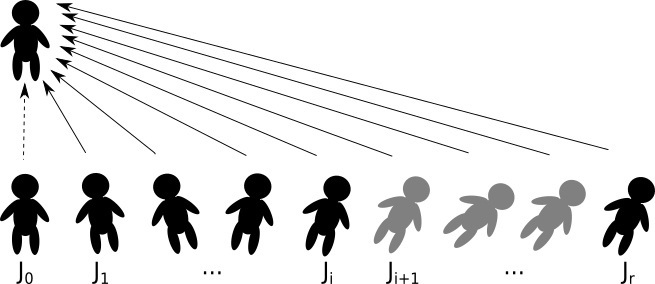
\includegraphics[width=.7\textwidth]{2/traditional-registration.png}
\caption{The traditional approach to volume registration in an rs-fMRI sequence consists of registering all volumes in the sequence to a single reference volume.}
\label{fig:ch4:traditional-reg}
\end{figure}

When performing image registration on a sequence of image volumes, one volume must be chosen as the reference volume for the entire sequence. All other volumes in the sequence are registered to this volume. An example of this process can be seen in Figure \ref{fig:ch4:traditional-reg}. In subsequent work, Friston et al. used the first volume in the rs-fMRI sequence as the universal reference image \cite{Friston1996}. Common choices for the reference volume include the volume with the least positional difference to all other volumes in the sequence, a volume produced by averaging all volumes in the sequence, or the first volume in the sequence \cite{Friston1996} \cite{Liao2005}. In our implementation, we chose to use the first volume in the sequence as the reference volume.

One drawback to this traditional approach to volume registration is that it only minimizes the differences between all the image volumes in the sequence and the reference volume. The keyword here is ``minimizes'': minimizing differences between image volumes does not mean that there are no differences between the image volumes. Image registration is an optimization problem, and its goal is to find the overlap between a pair of volumes with as few differences as possible either within a defined number of iterations or until the optimization cost does not change above a certain tolerance for a certain amount of time. These practical constraints on optimization problems mean that there may still be differences between other pairs of image volumes in the sequence that do not include the reference volume. 

Variations on Friston et al.'s framework have been developed over the last two decades. Liao et al. suggested that an rs-fMRI sequence could be viewed as a hidden Markov model, and reflected this idea in their suggested registration framework \cite{Liao2016}. They still use the first volume in the image sequence as the reference volume. Their framework uses the transformation of the previous volume to the reference volume to initialize the transformation for the current volume and the reference volume. 

It has been demonstrated that image registration across the entire image sequence reduces the effects of motion on the image sequence, though they do note that motion also affects the image due to changes in the spin history of the image. These effects are not correctable by global volume registration alone and will be discussed later in this chapter.

\subsection{Denoising}

Denoising techniques can be applied to an rs-fMRI after global volume registration is completed. They consist of regressions of various confounding variables. 

It is relatively common for researchers to use rigid realignment parameters calculated during volume registration as signals to remove via regression. The realignment parameters are the translations along and the rotations about the $x$, $y$, and $z$ axes \cite{Power2012}. These six parameters and their first-order derivatives are suggested as regression parameters by several researchers \cite{Power2012} \cite{Satterthwaite2012} \cite{VanDijk2012}. 

While the realignment parameters and their derivative for the current image volumes help reduce the effects of motion on an image sequence, these parameters are not sufficient on their own. As the effects of motion on rs-fMRIs have been studied, it has been established that motion at one point in the sequence can affect the next several volumes. Researchers have decided to address this effect by incorporating the rigid realignment parameters from surrounding timepoints into the regression parameters for any given current image volume \cite{Power2014} \cite{Satterthwaite2013} \cite{Yan2013a}.

Patriat et al. performed a robust comparison of different regression parameters on their MotSim motion data set \cite{Patriat2017}. They included rigid realignment parameters, but also used parameters obtained by performing principal component analysis (PCA) on the image sequences. PCA generates a set of linear, uncorrelated components that reflect the main features of a patient's motion. The list of parameter combinations included 
\begin{itemize}
\item 12mot: The six rigid realignment parameters and their first derivatives,
\item 12for: The first 12 principal components of the whole brain before realignment,
\item 12back: The first 12 principal components of the whole brain after realignment,
\item 12both: The first 12 principal components of the whole brain both before and after realignment,
\item 24mot: the six rigid realignment parameters of the current volume, the six rigid realignment parameters of the previous volume, and the square of these rigid realignment parameters,
\item 24both: the first 24 principal components of the whole brain before and after realignment.
\end{itemize}

\noindent They found that the features extracted from the image sequence using PCA explained more variance in the image sequence (measured using $R^2$) than the rigid realignment parameters. They showed that increasing the number of regressors increased the amount of variance explained, but with diminishing returns. While their work is promising, their experiment was performed on a simulated data set using healthy subject data and required an accurate estimate of the subject's head motion.

In addition to the positional effects of motion, the spin history and susceptibility effects of motion must be considered. Signals associated with these effects are called nuisance signals. One common nuisance signal is the global signal of the image sequence. Global signal regression (GSR) corrects for variance between temporal signals within a voxel and for the mean BOLD signal across all voxels \cite{Power2014} \cite{Satterthwaite2013} \cite{Yan2013} \cite{Yan2013a}. GSR has been shown to reduce spuriously increased long-distance correlations in functional connectivity studies, but may inadvertently weaken shorter-distance connections \cite{Jo2013} \cite{Power2014}  \cite{Satterthwaite2012}. Other nuisance signals that can be removed via regression are signals white matter and cerebral spinal fluid (CSF) \cite{Power2014} \cite{Satterthwaite2013}. The impact of removing these signals from the image sequence is limited: in some cases, removing white matter and CSF signals do not reduce the effects of motion on the BOLD signal \cite{Yan2013a} \cite{Jo2010}.

Another set of signals that may be removed via regression are components identified using techniques such as principal component analysis (PCA) or independent component analysis (ICA) \cite{Pruim2015} \cite{Salimi-Khorshidi2014} \cite{Behzadi2007}. Though both PCA and ICA decompose a set of data into a list of signals, the properties of the lists are different. PCA produces a list of orthogonal signals that best represent the features of a data set ordered from most representative to least representative. ICA treats the problem of decomposing the image sequence into different source signals as a blind source separation problem. ICA separates components by maximizing their statistical independence but requires additional help to identify the correct number of components. The set of components produced by ICA are assumed to be independent, non-Gaussian, and less complex than the original signal. For more details about ICA, refer to Section \ref{section:ica}. Regression of each of these sets of signals has been shown to reduce the effects of motion in the sequence, but neither removes them entirely \cite{Power2015} \cite{Parkes2017}. 

\subsection{Filtering}

Not all patients move in the same ways or at the same rate. In some cases, a patient will perform a large and sudden movement and then settle into a position close to their original position. The volumes containing the motion can be removed from the rs-fMRI sequence to create smaller, motion-free sequences. Several studies have found that subsequences of data of the same patient can be concatenated to produce a single, longer sequence without impacting the functional connectivity analysis. The process of detecting and removing motion-corrupted volumes has been formalized into several filtering techniques. 
Three popular filtering techniques are scrubbing, spike regression, and despiking. 

\textbf{Scrubbing} begins by examining the image sequence for ``high-motion'' image volumes \cite{Power2012}. Here, ``high-motion'' is defined as image volumes that have 0.5 mm FD and 0.5\% DVARS difference from their preceding volume. The volumes containing at least this quantity of motion, the preceding volume, and two subsequent volumes, are removed from the sequence, resulting in a set of discontinuous subsequences. The discontinuous subsequences can be combined without negatively impacting the functional connectivity analysis of the BOLD signal \cite{Fair2007} \cite{VanDijk2010}. As long as the reconnected subsequences compose a sequence at least 125 frames (approximately 5 minutes) in length, the scrubbed sequence can be used for analysis \cite{Power2012}. Many techniques for temporally filtering high-motion rs-fMRIs have been developed,  though all of them result in the loss of image volumes \cite{Barnes2011} \cite{Fransson2007} \cite{Jones2010} \cite{Kennedy2008} \cite{Smyser2010} \cite{Smyser2011}.  

\textbf{Spike regression} also identifies volumes containing large quantities of motion, though it treats them differently than scrubbing does. \cite{Satterthwaite2013}. It identifies spikes in the image sequence and replaces frames affected by the spikes with interpolated volumes.

A spike is defined as a frame in the sequence where the FD or the FD and the DVARS between it and its previous frame surpass a given set of thresholds. The value of the thresholds greatly impacts the cleaned image sequence. A low threshold will identify more spikes and produce a cleaner image sequence but remove more data, while a high threshold will retain more data but contain more motion artifacts. The thresholds used by Satterthwaite et al. on their adolescent data set are 0.25 mm FD and 1.4\% signal units of DVARS. 

After identifying the spikes in an image sequence, they are modeled as signals to remove through regression. The simplest model of a spike is as a motion event at a single time point. However, it has been established that patient motion may affect several frames in the image sequence. Satterthwaite et al. examined six combinations of frames around the frame in which the spike was based during their analysis of spike regression. They found that removing spikes identified using just the FD threshold and modeled as only effecting a single frame resulted in the fewest different neural connections in the highest and lowest motion images as well as the lowest correlation between functional connectivity and patient motion \cite{Satterthwaite2013}.

\textbf{Despiking} is different from these techniques. It treats the image sequence as a single image volume where each voxel contains an intensity signal. Each intensity signal is examined for sudden changes or spikes. The value of each detected spike is replaced with an interpolated value calculated using the preceding and subsequent points in the voxel's signal \cite{Jo2013} \cite{Patel2014}. Despiking does not remove volumes, but could accidentally remove valuable signals if they appear as outliers in the image voxel signals.

\subsection{Spin History Distortion Correction}

Many post-acquisition methods have been developed specifically to correct for distortions due to the impact of motion on the magnetic field. The usability of these dynamic distortion correction methods has been studied in a few specific cases, but their generalizability has yet to be confirmed in a broader range of fMRI studies \cite{Zaitsev2017}.

\section{Summary}

Resting-state fMRIs are four-dimensional images that record the BOLD signal in active areas of the brain. The BOLD signal can be used to evaluate the functional connectivity of different underlying networks in a patient's brain. Since rs-fMRIs are highly sensitive to motion, clinicians and psychologists have devised techniques to inform patients about what they can expect during an MRI scan as well as different coping mechanisms to help them remain calm during the scan. These techniques do not prevent the patient from moving, but approaches that do are not always appropriate to use during an rs-fMRI scan. Techniques and algorithms to prospectively and retrospectively remove motion from rs-fMRIs have also been developed, though they are not always successful in removing the effects of motion. Ultimately, the amount of motion present in the rs-fMRI sequence dictates whether or not the sequence can be used in clinical or research applications.
\chapter{METHODS: Motion Correction}
\label{ch:moco}

In the previous chapter, we discuss several techniques used to retrospectively correct motion. Motion correction pipelines may use denoising and filtering, but all pipelines begin with volume registration. In this chapter, we discuss a different approach to volume registration, how it compares to traditional volume registration, and how volume registration fits into a motion correction pipeline. 

%In this section, we discuss the two registration frameworks we apply to our rs-fMRIs: the traditional global volume registration framework and the DAG-based global volume registration framework. The registration frameworks will later be evaluated in comparison to each other, but will also be evaluated in the context of a complete motion correction pipeline. The motion correction pipeline of choice, ICA, will also be discussed in this section.

\section{Directed Acyclic Graph Based Volume Registration}

As discussed previously, the major drawback to Friston et al.'s approach to volume registration is that it only minimized the positional differences between the reference volume and the rest of the sequence. This drawback demonstrates an inability for the traditional approach to account for relationships in the patient's position throughout the scan. Intuitively, we know that the patient's position at any volume in the scan is more similar to his position in the immediately previous or subsequent volume than to another randomly chosen volume in the image.

In our proposed framework, we wish to account for these spatiotemporal relationships between temporally neighboring volumes in the sequence. To accomplish this goal, we start by viewing the rs-fMRI sequence as a directed acyclic graph (DAG). A DAG consists of a set of nodes and edges. Each edge has a direction associated with it and connects a pair of nodes. Since a DAG contains no cycles, there is no possible path back to a node once it has been traversed. 

\begin{figure}
\centering
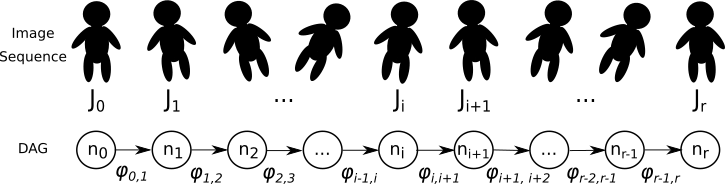
\includegraphics[width=.7\textwidth]{3/dag-chain.png}
\caption{A rs-fMRI can be viewed as a directed acyclic graph where each volume is a node and the edges connect from each volume $i$ to the following volume $i+1$.}
\label{ch3:fig:dag-chain}
\end{figure}

In the case of an rs-fMRI, each volume can be considered a node. The relationship between each pair of temporally neighboring volumes is represented as a directed edge connecting the node for the first volume to the node for the next volume. The acyclic nature of the DAG means that once a patient was in a specific position, he will never return to that exact same position with the exact same neurons firing. The position of the subject and his brain activity as measured by the BOLD signal may be similar in subsequent image volumes, but it will never be precisely the same. The perspectives of an rs-fMRI sequence as a set of images and of the sequence as a DAG can be seen in Figure \ref{ch3:fig:dag-chain}.

The cost of transitioning from one node to the next in our DAG has a parallel representation to the combination of the positional transformation needed to align volume $i$ to volume $i+1$ and the signal change between the volumes. This representation can be written as 

\begin{equation}
J_{i+1} = \phi_{i,i+1} J_i + \delta s_{i,i+1} + \epsilon
\end{equation}

\noindent{where $J_i$ and $J_{i+1}$ are volumes $i$ and $i+1$, $\phi_{i,i+1}$ is a matrix of transformation parameters that must be applied to $J_i$ to achieve the patient’s position in $J_{i+1}$, $\delta s_{i,i+1}$ is the natural change in BOLD signal, and $\epsilon$ is the change in BOLD signal due to motion. Currently, there is no way to estimate the natural change in BOLD signal and the change in BOLD signal due to motion without incorporating additional information about the MRI scanner and the patient that is not included in a rs-fMRI. We simplify our representation of the relationship between two volumes to}

\begin{equation}
J_{i+1} = \phi_{i,i+1} J_i + \epsilon^*
\end{equation}

\noindent{where $\epsilon^*$ is the change in the BOLD signal that cannot be accounted for after aligning the patient’s position in the two volumes. Here, we use the notation $\epsilon^*$ to represent the generic error change in BOLD signal across any pair of volumes.}

After aligning two volumes $i$ and $i+1$, we will then align volumes $i+1$ and $i+2$:

\begin{equation}
\begin{split}
J_{i+2} & = \phi_{i+1,i+2} J_{i+1} + \epsilon^* \\
& = \phi_{i+1,i+2} (\phi_{i,i+1} J_i + \epsilon^*) +\epsilon^*\\
& = \phi_{i+1,i+2} \phi_{i,i+1} J_i + \epsilon^{*'}\\
\end{split}
\end{equation}

\noindent Traditional volume registration assumes that 

\begin{equation}
\phi_{i,i+2} = \phi_{i+1,i+2} \phi_{i,i+1}
\end{equation}

\begin{figure}
\centering
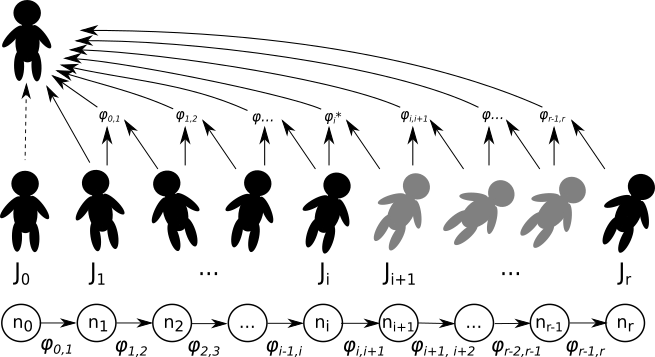
\includegraphics[width=.7\textwidth]{3/dag-registration.png}
\caption{The traditional approach to volume registration in an rs-fMRI sequence consists of registering all volumes in the sequence to a single reference volume.}
\label{ch3:fig:dag-reg}
\end{figure}

\noindent{and calculates $\phi_{i,i+2}$ directly. We argue that this assumption is not true in all cases. Rather than directly calculate $\phi_{0,i}$ and use it to align volume $i$ to the reference volume as the traditional method does, we calculate each component $\phi$ that is a factor of $\phi_{0,i}$. Each component $\phi_{i,i+1}$ is combined with the preceding $\phi_{0,i}$s to recursively align volume $i+1$ to the reference volume without making the large and often inaccurate transformations required by directly calculating $\phi_{0,i+1}$.} This process is outlined in Figure \ref{ch3:fig:dag-reg}.

\section{Independent Component Analysis}

The purpose of image registration is purely to ensure the position of the patient throughout the entire rs-fMRI is consistent. After registration, the image still contains BOLD source signals and noise signals caused by factors other than brain activity. The challenge of separating these combined signals is called blind source separation (BSS). 

We chose to focus on an independent component analysis (ICA) approach for solving the BSS problem. The specific technique we use has been described by Beckmann and Smith as probabilisic ICA. This section aims to provide an overview of the probabilistic ICA technique. For further details, please refer to the technical reports by the FMRIB group \cite{Beckmann2004} \cite{Woolrich2004} \cite{Beckmann} \cite{Smith2004}.

Probabilistic ICA is a linear regression model which performs mixing in the original data space and assumes the true BOLD signal has been confounded by Gaussian noise. These constraints mean that BSS can be solved in three steps:

\begin{enumerate}
\item Estimate a joint subspace consisting of source and noise signals and an noise subspace orthogonal to the joint subspace,
\item Estimate the independent sources in the joint subspace, and 
\item Assess the statistical significance of the independent sources.
\end{enumerate} 

Probabilistic ICA treats the voxel intensity values in every frame of the image sequence as a matrix of $V$ voxels across $n$ time points. For each voxel $v_i \in V$, the observed signal in that voxel can be modeled as

\begin{equation}
\label{ch3:eq:ica01}
\vec{x_i} = A \vec{s_i} + \mu + \vec{\eta_i}
\end{equation}

\noindent This equation allows three different types of signals to contribute to the observed voxel values $\vec{x_i}$ for a given voxel across all $n$ timepoints in the sequence. The first type of signal is a vector of non-Gaussian source signals $\vec{s_i}$ across all $n$ timepoints. The source signals are modulated by mixing matrix $A$ whose shape is the number of time points $n$ by the number of source signals $q$. The second type of signal is an offset denoted by $\mu$. The offset constrains the observed signals to be centered around the mean of all observed signals. The third type of signal $\vec{\eta_i}$ is a vector of noise throughout the duration of the sequence. To summarize, probabilistic ICA explicitly assumes that the observed signal in a given voxel can be divided into non-Gaussian source signals, isotropic Gaussian noise signals, and some offset. This assumption makes it easier to separate a source signal from a noise signal: a noise signal will have a Gaussian distribution while a source signal will not. \textbf{The goal of probabilistic ICA is to identify the source signals, $\vec{s}$.}

With this combination of signals in mind, we can write the covariance matrix of the observed data $x$ as

\begin{equation}
\label{ch3:eq:cov-01}
R_x = \langle x_i x_i^T \rangle = AA^T + \sigma ^2 I
\end{equation}

\noindent where $A$ is the mixing matrix, $\sigma^2$ is the standard deviation of the noise, and $I$ is $n$x$n$ identity matrix. The covariance matrix of the observed data $R_x$ can be calculated, but $A$ and $\sigma^2$ are both unknown. The noisy observed data is transformed with respect to the noise sources using a process called whitening. The whitening with respect to noise enforces the assumption of noise following an isotropic Gaussian distribution with a mean of zero and a standard deviation of $\sigma^2$.

The mixing matrix $A$ can be estimated using maximum likelihood estimation. Beckmann and Smith use singular value decomposition of the observed data $X = U(N\Lambda)^{\frac{1}{2}} V$ to model the estimator of $A$:

\begin{equation}
\hat{A}_{ML} = U_q(\Lambda_q - \sigma ^2 I_q)^{\frac{1}{2}}Q^T
\end{equation}

\noindent where $U_q$ contains the eigenvectors associated with the $q$ largest eigenvalues, $\Lambda_q$ contains the $q$ largest eigenvalues, and $Q$ is a $q$x$q$ orthogonal rotation matrix in the whitened observation space such that $QQ^T = I$. %This estimator assumes that the number of source signals $q$ is known. In a noiseless system, the number of source signals is equivalent to the rank of the covariance matrix of the observed data. However, rs-fMRIs are inherently noisy. In this more general case, the number of sources is more complex to determine. Beckmann and Smith suggest that the number of source signals is the same as the number of eigenvalues of the covariance matrix that violate the ``sphericity assumption of the isotropic Gaussian noise model'' \cite{Beckmann2004}. 
The eigenvectors and eigenvalues can be calculated from $X$, but $\sigma$ and $Q$ remain unknown. As noted earlier, the matrix $Q$ is an orthogonal rotation matrix which, when applied to the whitened data $\tilde{x}$, has the same effect of applying an unmixing matrix to the observed data: 

\begin{equation}
\label{ch3:eq:unmixing-01}
W \vec{x} = Q \tilde{x} = \hat{s}
\end{equation}

\noindent Both matrix-vector multiplications serve to estimate individual source signals $\hat{s}$. The estimated source signals are identified by projecting the whited data $\tilde{x}$ onto each row $r$ of the unmixing matrix $Q$ a total of $q$ times:

\begin{equation}
\hat{s_r} = Q_{r,:} \tilde{x}
\end{equation}

\noindent where the $Q_{r, :}$ represents row $r$ of matrix $Q$.  \textit{(Note: A key assumption in this step is that the rows of the unmixing matrix are mutually orthogonal so that they cover the entire space of signal sources. Additional steps described by Beckmann and Smith can be taken to incoporate prior information about the voxels into this step \cite{Beckmann2004}.)}

At this point, the standard deviation of the noise $\sigma^2$ and the source signals are unknown. We can solve the following system of equations jointly to resolve these two unknown quantities:

\begin{equation}
\hat{s}_{ML} = (\hat{A}^T\hat{A})^{-1}\hat{A}^Tx = \hat{W}x = Q \tilde{x}
\end{equation}

\begin{equation}
\hat{\sigma}_{ML}^2 = \frac{1}{n-q} \sum_{l=q+1}^p \lambda_l .
\end{equation}

Solving these equations is an iterative process. First, the mixing matrix and source signals are estimated. These estimations are used to calculate the corresponding estimator of the standard deviation of the noise. Then, the residual noise $\hat{\eta}_i$ at each voxel $v_i$ is calculated:

\begin{equation}
\label{ch3:eq:res-01}
\hat{\eta}_i = (I - \hat{W}^T\hat{W}) x_i.
\end{equation}

\noindent Recalling from Equation \ref{ch3:eq:ica01} how probabilistic ICA views a signal, Equation \ref{ch3:eq:res-01} becomes: 

\begin{equation}
\hat{\eta}_i = (I - \hat{W}^T\hat{W}) A + (I - \hat{W}^T\hat{W}) \eta
\end{equation}

When the correct number of sources has been identified, the estimated mixing matrix will fully span the source signal space. Then, the residual noise will only be related to the true noise:

\begin{equation}
\hat{\eta}_i = 0 + (I - \hat{W}^T\hat{W}) \eta
\end{equation}

Upon reaching this stage in the probabilistic ICA technique, the source signals have been approximated. The source signals are called spatial independent component maps. Normalizing the values in these maps by the variance of the noise produces $Z$-statistic maps. $Z$-statistic maps can be analyzed to identify voxels with statistically significant activations. These activations are attributed to BOLD signal.

One of the major limitations of ICA is that it is highly data driven. It assumes the dataset contains a sufficiently large number of images, each with a sufficiently large number of voxels. Even assuming an ideal data set, the true value of the mixing matrix is dependent on the observed data \cite{Beckmann2004}. Fluctuations in the data can lead to deviations of the residual noise in certain voxels from the true noise. These deviations can produce \textit{type-I} and \textit{type-II} errors when examining the $Z$-statistic maps to identify statistically significantly activated voxels.
 
Additionally, the developers of probabilistic ICA note that not all noise follows the isotropic Gaussian assumption. Noise based in the patient's physiology is likely to be structured in a way that is non-Gaussian. The non-Gaussian noise signals can still be separated from the BOLD source signals, but only if these noise signals are not highly correlated with the source signals.

\section{Motion Correction Pipeline and Implementation}

Both the traditional and novel volume registration techniques were applied independently to each image from the subject cohorts described in Chapter \ref{ch:data}. After registration, three versions of each image existed: the original BOLD sequence, the sequence modified using traditional volume registration, and the sequence modified using the novel registration method.

The registration algorithms applied to rigid tissue types used affine registration with two degrees of granularity. When applied to soft tissue types (ie, placenta),  three nonlinear transformations with increasing granularities were performed after the affine registrations. The exact parameters used for each volume registration can be seen in Appendix A\ref{appendix:registration-params}. The registration frameworks were implemented in Python using the nipype (Neuroimaging in Python Pipelines and Interfaces) library \cite{Gorgolewski2011}. Volume registration used the ANTs (Advanced Normalization Tools) tools as a backend \cite{Avants2014}.

After performing volume registration to ensure the patient is in the same physical space throughout the image sequence, the image sequence may still contain artifacts due to motion. Our registered sequences underwent motion correction via a well-established motion correction pipeline. We chose to use the independent component analysis (ICA) pipeline outlined by Beckmann and Smith \cite{Beckmann2004}. The motion corrected sequences produced by FMRIB's MELODIC tool were saved alongside the original and registered sequences.  

\section{Evaluating Registered and Motion Corrected Sequences Against Gold Standard Usability Thresholds}

The main goal of motion correction is to reduce the effects of motion on the image so that it is usable. The gold standards for rs-fMRI usability as established by Power et al. are that the FD and DVARs metrics must change less than 0.2 mm and 2.5\% normalized voxel units between at least 50\% of the neighboring volumes. The FD and DVARs metrics between each pair of subsequent image volumes were calculated for the original, registered, and motion corrected sequences. The metrics for each sequence were then compared to the gold standard image usability thresholds. This comparison answers the key question of how each registration framework impacts an established motion correction pipeline.

Additionally, a smaller comparison of the registered sequences was conducted. This comparison evaluates the immediate impact of the registration algorithm on the image sequence. It is highly unlikely that an entire image sequence would meet the Power et al. usability thresholds after only the initial step of a motion correction pipeline, but it is valuable to examine the impact of a volume registration algorithm at each stage of the pipeline. 

\textbf{Implementation.} We calculated the FD and DVARS metrics defined by Power et al. using the FSLMotionOutliers tool \cite{Power2012}. 


\chapter{METHODS}
\label{ch:methods}

\section{Volume Registration Frameworks}

In this section, we discuss the two registration frameworks we apply to our rs-fMRIs: the traditional global volume registration framework and the DAG-based global volume registration framework. The registration frameworks will later be evaluated in comparison to each other, but will also be evaluated in the context of a complete motion correction pipeline. The motion correction pipeline of choice, ICA, will also be discussed in this section.

It has been demonstrated that image registration across the entire image sequence reduces the effects of motion on the image sequence, though they do note that motion also effects the image due to changes in the spin history of the image. These effects are not correctable by global volume registration alone. % and are addressed later in this chapter.

\subsection{Traditional Volume Registration}

The rs-fMR image is stored in computer memory as a set of 3D matrices. The values in corresponding cells of each matrix are considered to be aligned in this digital space (voxel space). The voxel space is defined by the imaging protocol and relates to the physical space through the spatial resolution of the image. Even though the spatial and voxel spaces for the image align, the contents of the image volumes may be misaligned due to patient movement. Because we cannot assume that an image is completely motion-free, we cannot directly compare the contents of each image volume in the rs-fMRI sequence. However, we can use image registration to align the contents of the image volumes to reduce the impact of motion on patient position.

Image registration is the process of morphing the contents of one image so that they overlap optimally with another image. The morphing operations include translation, rotation, scaling, skewing, and nonlinear adjustments. The linear and affine operations in this list should be used to perform rigid body registrations for organs such as the brain. Nonlinear operations can be used to fine-tune the alignment of more pliable organs such as the liver. All morphing operations are applied to one image (the moving image) repeatedly until it's contents optimally match those of the static reference image as determined by a chosen similarity metric. 

One of the earliest examples of image registration was described by Friston et al. in 1995 \cite{Friston1995}. They performed image registration on positron emission tomography (PET) scans and MRI scans of a human brain. During the registration process, one scan was designated as the ``reference'' image, which remained stationary, and the other scan was designated as the ``object'' image, which was transformed to match the reference image. Constraining the alignment process to transforming a single image into the coordinates of the other image rather than transforming both images into an independent coordinate frame simplifies the registration process.

When performing image registration on a sequence of image volumes, one volume must be chosen as the reference image for the entire sequence. In subsequent work, Friston et al. used the first volume in the rs-fMRI sequence as the universal reference image \cite{Friston1996}. Common choices for the reference volume include the volume with the least FD to all other volumes in the sequence, a volume produced by averaging all volumes in the sequence, or the first volume in the sequence [Friston et al. (1996); Liao et al. (2005)]. In our implementation, we chose to use the first volume in the sequence as the reference volume.

One drawback to Friston et al.'s volume registration framework is that it only minimizes the differences between all the image volumes in the sequence and the reference volume. The key word here is minimizes: minimizing differences between image volumes does not mean that there are no differences between the image volumes. Image registration is an optimization problem, and its goal is to find the overlap between a pair of volumes so that there are as few differences as possible either within a defined time period or until the optimization cost does not change above a certain tolerance for a certain amount of time. These practical constraints on optimization problems mean that there may still be differences between other pairs of image volumes in the sequence that do not include the reference volume. 

%Variations on Friston et al.'s framework have been developed over the last two decades. Liao et al. suggested that a rs-fMRI sequence could be viewed as a hidden Markov model, and reflected this idea in their suggested registration framework \cite{Liao2016}. They still use the first volume in the image sequence as the reference volume. Their framework uses the transformation of the previous volume to the reference volume to initialize the transformation for the current volume and the reference volume. 

%The success of volume registration in an rs-fMRI sequence is defined by the framewise differences between temporally neighboring image volumes.  During the registration process, the three translation and three rotation parameters can be used to calculate the displacement between a pair of images, which is often referred to as the framewise displacement (FD). Three groups have proposed slightly different methods for calculating the FD: Power et al., Jenkinson et al., and DOsenbach et al. \cite{Power2012} \cite{Jenkinson2002} \cite{Dosenbach2017}. All three FD calculations produce correlated metrics: the FD metric proposed by Power et al. produces measurements approximately twice as large as the metric proposed by Jenkinson et al., and Dosenbach et al. reported a high correlation between their FD and Power's FD \cite{Yan2013a} \cite{Dosenbach2017}.

%The FD metric only measures the positional effects of motion, not the variations in signal in individual voxels caused by motion. Changes in signal between volumes can be measured using the temporal derivative of the variance in the BOLD signal intensity (DVARS) between neighboring volumes \cite{Power2012} \cite{Smyser2015}. DVARs is an effective measure of the spin gradient effects of motion because it measures the change in BOLD signal intensity, which is highly related to motion-induced spin gradient changes. 


% This framework only minimizes the differences between the reference volume and the other volumes in the sequence, not the differences between other pairs of volumes. If the rs-fMRI sequence contains too much motion between frames as exhibited in Figure 1a, the traditional global volume registration framework will produce a sequence containing volumes with even more motion between frames than the original sequence.

\subsection{Directed Acyclic Graph Based Registration}

In our proposed framework, we wish to account for the spatiotemporal relationships between temporally neighboring volumes in the sequence. To accomplish this goal, we start by viewing the rs-fMRI sequence as a directed acyclic graph (DAG). A DAG consists of a set of nodes and edges. Each edge has a direction associated with it and connects a pair of nodes. Since a DAG contains no cycles, there is no possible path back to a node once it has been traversed. 

In the case of a rs-fMRI, each volume can be considered a node. The relationship between each pair of temporally neighboring volumes is represented as a directed edge connecting the node for the first volume to the node for the next volume. The acyclic nature of the DAG means that once a patient was in a specific position, he will never return to that exact same position with the exact same neurons firing again. The position of the subject and his brain activity as measured by the BOLD signal may be similar in subsequent image volumes, but it will never be precisely the same. The parallel perspectives of an rs-fMRI sequence as a set of images and of the sequence as a DAG can be seen in Figure 1b.

The cost of transitioning from one node to the next in our DAG has a parallel representation to the combination of the positional transformation needed to align volume $i$ to volume $i+1$ and the signal change between the volumes. This representation can be written as 

\begin{equation}
J_{i+1} = \phi_{i,i+1} J_i + \delta s_{i,i+1} + \epsilon
\end{equation}

\noindent{where $J_i$ and $J_{i+1}$ are volumes $i$ and $i+1$, $\phi_{i,i+1}$ is a matrix of transformation parameters that must be applied to $J_i$ to achieve the patient’s position in $J_{i+1}$, $\delta s_{i,i+1}$ is the natural change in BOLD signal, and $\epsilon$ is the change in BOLD signal due to motion. Currently, there is no way to estimate the natural change in BOLD signal and the change in BOLD signal due to motion without incorporating additional information about the MRI scanner and the patient that is not included in a rs-fMRI. We simplify our representation of the relationship between two volumes to}

\begin{equation}
J_{i+1} = \phi_{i,i+1} J_i + \epsilon^*
\end{equation}

\noindent{where $\epsilon^*$ is the change in the BOLD signal that cannot be accounted for after aligning the patient’s position in the two volumes. Here, we use the notation $\epsilon^*$ to represent the generic error change in BOLD signal across any pair of volumes.}

After aligning two volumes $i$ and $i+1$, we will then align volumes $i+1$ and $i+2$:

\begin{equation}
\begin{split}
J_{i+2} &= \phi_{i+1,i+2} J_{i+1} + \epsilon^* \\
&= \phi_{i+1,i+2} (\phi_{i,i+1} J_i + \epsilon^*) +\epsilon^*\\
&= \phi_{i+1,i+2} \phi_{i,i+1} J_i + \epsilon^{*'}\\
\end{split}
\end{equation}

Traditional volume registration assumes that 

\begin{equation}
\phi_{i,i+2} = \phi_{i+1,i+2} \phi_{i,i+1}
\end{equation}

\noindent{and calculates $\phi_{i,i+2}$ directly. We argue that this assumption is not true in all cases. Rather than directly calculate $\phi_{0,i}$ and use it to align volume $i$ to the reference volume as the traditional method does, we calculate each component $\phi$ that is a factor of $\phi_{0,i}$. Each component $\phi_{i,i+1}$ is combined with the preceding $\phi_{0,i}$s to recursively align volume $i+1$ to the reference volume without making the large and often inaccurate transformations required by directly calculating $\phi_{0,i+1}$.}


\section{Pattern Detection}

%The global volume registration techniques were applied to all 17 resting-state BOLD MR images. After the registrations, each subject had three sequences associated with it: the original sequence, the sequence registered using the traditional framework, and the sequence registered using the DAG-based framework. The globally registered images were compared to each other in terms of correlation ratios between all volumes in the sequence as well as FD and DVARS between temporally neighboring volumes. 

%The correlation ratio is an asymmetrical, spatially informed measure of the overlap between images where volumes with better alignment will have lower correlation ratios \cite{Roche1998}. For each sequence, we used FLIRT (FMRIB’s Linear Image Registration Tool) to calculate the correlation ratio between each possible pair of volumes in the sequence \cite{Jenkinson2001} \cite{Jenkinson2002}. We then used the average and standard deviation of the correlation ratio distribution of each image to compare the images. We also calculated the FD and DVARS metrics defined by Power et al. using the FSLMotionOutliers tool \cite{Power2012}. These metrics were calculated for each image and were used for evaluation of the efficacy of the registration frameworks.

\section{Metrics and Analyses}

Power et al. thresholds

Correlation ratio matrix

Statistical tests

Dice coefficients?

\section{Implementation: Tools and Libraries}

%Both registration frameworks described in this section were implemented in Python using the nipype (Neuroimaging in Python Pipelines and Interfaces) library \cite{Gorgolewski2011}. Affine volume registration was performed using ANTs (Advanced Normalization Tools) \cite{Avants2014}. The metric used to estimate the dissimilarity between the pairs of volumes being registered was cross-correlation with a local window size of 5 voxels. 

Cite nipypy, ANTs, FSL, etc. here


\chapter{DATA}
\label{ch5:data}

The data used to test the hypothesis and aims introduced in the previous chapter are drawn from four clinical groups and  a set of simulated rs-fMRI sequences. In this chapter, we will first discuss the clinical images, which were taken from several prospective studies of congenital heart defects in pediatric patients as well as a prospective study of Alzheimer's disease in an aging population. Subjects from these studies were chosen because patient motion causes problems in MR images for the entire patient lifespan, though patients may exhibit different types of motion at different stages of life. 

Then we will discuss how we overcame the lack of objective ground truth in medical imaging research by developing a mechanism to simulate brain activity, scanner noise, and motion in rs-fMRI sequences.

\section{Clinical Cohorts}

The phrases congenital heart defects (CHDs) and congenital heart disease (CHD) both refer to defects in the heart or the vessels around the heart. CHDs affect how blood moves into, through, and away from the heart. 
CHD has a worldwide prevalence of about 8 per 1000 live births, meaning about 1.35 million children are born with CHD every year. %Since the survivability of CHD has increased from 10\% to 90\%, the medical community is faced with a growing, aging population of CHD patients. 

In this section, we provide a general overview of the impact of CHD on a global scale, the process for diagnosis, and additional risks associated with CHD. We then discuss the process of diagnosing neurodevelopmental comorbidities occurring with CHD and the impact of improved medical care on the CHD population. We end this section with a description of the four populations from which we obtained clinical rs-fMRI sequences.


\subsection{CHD Background}

\begin{figure}
\centering
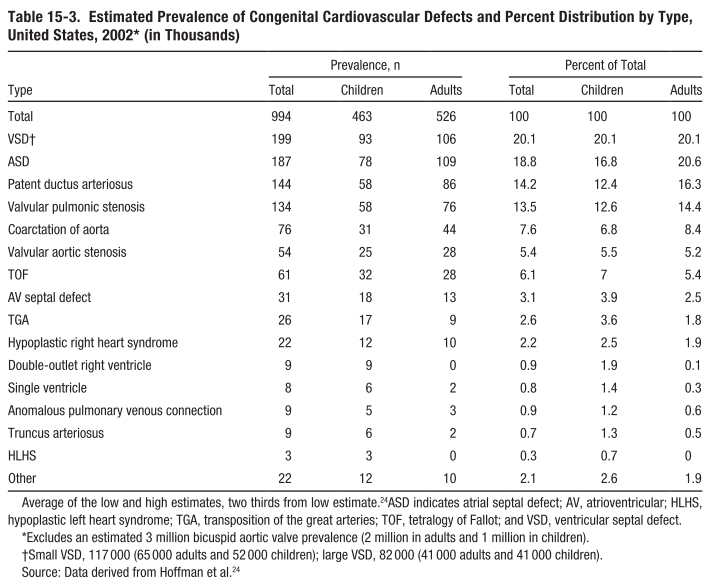
\includegraphics[width=0.6\textwidth]{5/chd-defects-usa.png}
\caption{Table of prevalences of congenital heart defects borrowed temporarily from \cite{Mozaffarian2016}.}
\label{ch5:fig:usa-defects-prev}
\end{figure}

CHD consists of a variety of defects which can affect any combination of the vessels and chambers of the heart with varying degrees of severity. The defects prevent the cardiopulmonary system as a whole from functioning correctly, but pinpointing and treating the defects effectively can be a complex process. It is important to note that each defect type has a different prevalence, a different treatment plan, and different expected outcomes. A breakdown of prevalence rates of some of the most common lesion types can be seen in Figure \ref{ch5:fig:usa-defects-prev}. % See (16)

% Causes of CHD: genetic syndromes, single gene mutations, environmental exposure, and unknown
Different presentations of CHD are associated with a number of different genetic and environmental factors \cite{Mozaffarian2016}. Genetic conditions such as Down syndrome, Turner syndrome, 22q11 deletion syndrome, Williams syndrome, and Noonan syndrome are associated with certain CHD presentations. Maternal behaviors such as smoking and binge drinking are known to cause heart problems in the fetus. Other maternal risk factors are obesity, folate deficiency, and living at a high altitude. Paternal exposure to phthalates, anesthesia, sympathomimetic medications, pesticides, and solvents may increase the risk of the fetus for developing CHD. While there are quite a few factors in this list, there are many CHD cases whose causes are unknown.

Once a patient is diagnosed with one of these defects or a cause of the CHD is identified, the specific nature of his case must be clearly documented. The documentation of CHD using the International Classification of Diseases, Ninth Revision, Clinical Modification (ICD-9-CM) has 25 high level codes representing various presentations of CHD, but these codes used alone are often not sufficient for describing a patient's true condition \cite{Mozaffarian2016}. Additional ICD-9-CM codes should be used to communicate the finer details of a patient's condition, if they are available. %something about how ICD codes make it easier to

The incidence of CHD in live births vary across countries and continents. The United States reports approximately 4-10 CHD case per 1000 live births. Europe and Asia see about 6.9 and 9.3 CHD cases per 1000 live births, though smaller studies have been conducted in many countries to measure local prevalence \cite{Mozaffarian2016}. In China, the incidence of CHD ranges from 8.98 to 11.1 per 1000 live births \cite{Zhao2019} \cite{Qu2016}. 
A pair of studies from Iran report incidences of 8.6 and 12.3 per 1000 live births, though the studies note that they were performed in different geographical locations with different populations within the country \cite{Nikyar2011} \cite{Rahim2008}.
One report from Dharan reports an incidence of 5.8 per 1000 patients admitted to a tertiary care hospital over a 12 month period \cite{Shah2008}. A study of newborns at one hospital in New Delhi, India claims an incidence of 3.9 per 1000 live births, though this rate may be a poor estimate as there is a significant delay between patient birth and referral to a cardiac center in India \cite{Khalil1994} \cite{Saxena2005}.

These incidence rates should be analyzed with some caution. In many cases, the reported rates were based on medical records. Medical records are not always correct; it is well known that human error can lead to a medical record lacking information or containing incorrect information. The only way for a person to have a medical record is for him or her to go to a medical center. Not everyone who has CHD is able to seek medical help, often because of their geographical locations or their income. Even if a patient is able to seek medical help, the availability of proper cardiac care varies between and within countries. However, it is generally expected that CHD incidence rates will increase as screening tools and treatments become more effective and more widespread, leading to earlier detection of defects.
 
% Diagnosis
Currently, the process of detecting and diagnosing CHD can begin before birth. A specialized ultrasound test called fetal echocardiography can detect heart abnormalities as early as the second trimester of the pregnancy. People who learn they are pregnant with a fetus who shows signs of CHD may choose to handle this information by opting for termination or pursuing a more detailed diagnosis. Additional tests, such as amniocentesis and follow-up ultrasounds may be used to determine treatment options before the patient is born. Generally, severe CHD cases present and are detected at earlier stages of life, but minor defects may not become apparent until the patient is older. Tests used to diagnose CHD in postnatal patients include electro- and echo-cardiograms, chest x-rays, pulse oximetry, exercise stress tests, computed tomography or MRI scans, and cardiac catheterization. Treatment of different defects varies from monitoring and medication to surgery and cardiac implants.

\begin{figure}
\centering
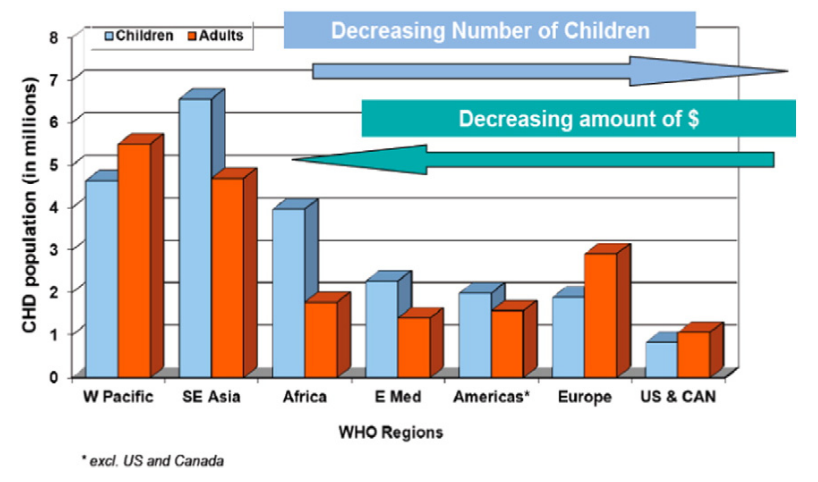
\includegraphics[width=0.7\textwidth]{5/CHD-burden-webb.png}
\caption{Estimated CHD burden in World Health Organization (WHO) regions using incidence rates of approximately 12/1000 and 4/1000 in children and adults, respectively \cite{Webb2015}.}
\label{ch5:fig:CHD-burden}
\end{figure}

%Depending on the cause of the 
The cost of diagnostic techniques and treatment plans impose different levels of financial burden on CHD patients and their families. Certain defects require complex, expensive surgical repairs while others can be treated with less expensive approaches \cite{Mozaffarian2016}. The burden of CHD across the globe was outlined by Webb et al \cite{Webb2015}. Their figure illustrating the prevalence of CHD and the availability of funds with which to treat it can be see in Figure \ref{ch5:fig:CHD-burden}. As the overall mortality of CHD declines, the burden of CHD is expected to increase \cite{Mozaffarian2016}.

% Complications and risks
Unfortunately, the cost of treating CHD is not the only burden a patient must undergo. Patients with CHD are also at increased risk for heart failure and infections \cite{Mozaffarian2016}. Children with CHD are at 19-fold risk for stroke compared to their healthy counterparts \cite{Fox2015}. In a study of Swedish citizens born between 1970 and 1993, Giang et al compared the prevalence of cardiac conditions in patients with and without CHD \cite{Giang2018}. They found that patients who had a CHD diagnosis were at about eight times higher risk for intracerebral hemorrhage and subarachnoid hemorrhage than their non-CHD counterparts. The CHD patients were also more likely to suffer from arrhythmia and heart failure. 

% When are patients diagnosed?
% Expected lifespan
% Treatment plan
% Financial burden

However, cardiac conditions are not the only complications CHD must deal with. Many of these patients also suffer from neurocognitive disorders that co-occur with CHD. Early research in this area focuses on the neurodevelopmental status of neonatal patients pre- and post-surgical intervention. One theory was that some factor or factors in the surgical intervention caused brain injuries in the patients. This idea proved to be inaccurate when researchers began detecting neurological malformations \textit{in utero}.

In a systematic review of available literature regarding prenatal and postnatal presurgical CHD cases and neurodevelopmental outcomes, Mebius et al. identify two theories about the causality of  neurodevelopmental delays and CHD \cite{Mebius2017}. The first theory is that abnormalities in the cardiac system prevent the developing brain from receiving enough oxygen and nutrients, which disrupts prenatal brain development. The second theory is that faulty genetic pathways used during both cardiac and brain development cause both conditions to co-occur. However, 11 articles Mebius et al. found during their review that are related to bloodflow through the umbilical artery suggest a third theory. During the prenatal period, a fetus receives oxygen from the mother via the placenta. If the placenta was not functioning correctly, it could lead to the fetus receiving not enough oxygen. Lower quantities of oxygen throughout prenatal development could potentially cause problems both in brain and cardiac growth. The 11 articles have contradictory results, but some researchers are currently investigating the role of the placenta in CHD and prenatal brain development.

Survival of CHD patients to adulthood has increased from 10\% to 90\% over the last several decades as CHD diagnostic tools and treatments have improved.  Currently, Webb et al. estimate that at least 12 to 34 million adults have CHD, and this number is expected to increase \cite{Webb2015}. The impact of the combination of CHD and neurological conditions throughout a patient's lifetime is starting to be explored. The aging of the CHD population has also sparked interest in the relationships between CHD and adult-stage neurological disorders such as dementia and Alzheimer's. 

While the purpose of this study is not to focus on CHD patients, we chose to use CHD and aging brain images in support of research being performed in the area of relationships between CHD and neurodevelopment.

%To address:
%\begin{itemize}
%\item Common combinations
%\item Joint treatment?
%\item Additional risks?
%\item Joint financial and emotional burden on caretakers? 
%\item CHD, neuro, and aging? Dementia/Alzheimer's? Recent data ... MIND neuroimaging ancillary r01 dec 17
%\end{itemize}


\subsection{Identifying Neurocognitive Disorders}

Neurocognitive disorders are usually diagnosed using at least one of many psychological survey-based evaluations, but these methods are subjective. rs-fMRIs could be used to identify patients who have functional connectivity patterns associated with different neurocognitive disorders, and eventually may be used to identify patients who are at risk for developing these disorders.

\subsubsection{Patient Surveys}

Surveys known to be used for studying the relationship between CHD and neurodevelopment are

\begin{itemize}
\item National Institute of Health Toolbox (3 - 85 years): ``Performance tests of cognitive, motor, and sensory function and self-reported measures of emotional function for adults and children in the general population and those living with a chronic condition''.

\item Sue Beers (4 - 18 years [not inclusive of 18 years]): WASI-II, NEPSY-2, WRAML-2, D-KEFS, WISC-IV, Grooved Pegboard, BRIEF, Beery-Buktenica VMI, ASRS, Conners-3, BASC-II, ABAS-II, PedsQL General, PedsQL Cardiac, Pictoral Scale Self Perception Profile.

\item SVR-III NDT (9 - 13 years [not inclusive of 13 years]): WIAT, NEPSY, WRAML, D-KEFS, WISC-V, Grooved Pegboard, BRIEF, Beery-Buktenica VMI, ASRS, Conners ADHD Index, BASC-II, ABAS-3, PedsQL General, PedsQL Cardiac

\item Bayley Scales of Infant and Toddler Development -III (1 - 24 months): Subtests include cognitive, language, social-emotional, motor, and adaptive behavior tests \cite{Mebius2017}.

\item Battelle Developmental Inventory (Birth - 8 years [not inclusive of 8 years]): Subsets include cognition, communication, social-emotional development, physical development, and adaptive behavior.

\item Developmental Assessment of Young Children (Birth - 6 years [not inclusive of 6 years]): Subtests include cognition, communication, social-emotional development, physical development, and adaptive behavior.

\item Preschool Language Scale + Receptive-Expressive Emergent Language (Birth - 3 years): Total language, auditory comprehension, expressive communication, articulation, receptive language, expressive language, and inventory of vocabulary words.

\item Peabody Developmental Motor Scales (Birth - 5 years): Subtests include reflexes, stationary, locomotion, object manipulation, grasping, visual-motor integration
\end{itemize}

The goal of these surveys is to compare the patient's cognitive function and neurological functions to expected milestones. Certain deviations from certain milestones are indicative of different disorders.

\subsection{Study Cohorts}

The rs-fMRIs used in this study were gathered as part of ongoing studies of the relationship between CHD and neurodevelopment. Data from the CHD/neurodevelopment studies was obtained through studies approved by the IRB at the Children's Hospital of Pittsburgh of UPMC and the University of Pittsburgh. All data is stored and accessed in compliance with HIPPA policies.

The subjects included in this analysis fall into three age groups: neonatal, preadolescent, and fetal. To summarize the cohorts, there were 163 brain rs-fMRIs obtained for the neonatal cohort, 546 brain rs-fMRIs obtained for the preadolescent cohort, and 124 brain rs-fMRIs obtained for the fetal cohort. The fetal cohort also contains 106 rs-fMRIs of the placenta. The race, ethnicity, and gender counts for these three cohorts can be seen in Figures  In the following sections, we describe each cohort in detail. 

\begin{figure}
\centering
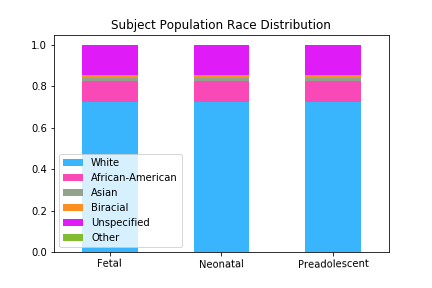
\includegraphics[width=.75\textwidth]{5/demo_clinical_subj_race.png}
\caption{Distribution of subject races for all three cohorts.}
\label{ch5:clinical:race}
\end{figure}%
%
\begin{figure}
\centering
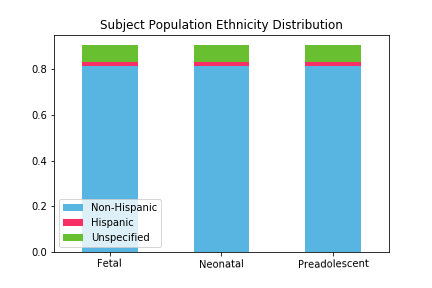
\includegraphics[width=.75\textwidth]{5/demo_clinical_subj_ethnicity.png}
\caption{Distribution of subject ethnicities for all three cohorts.}
\label{ch5:clinical:eth}
\end{figure}

\begin{figure}
\centering
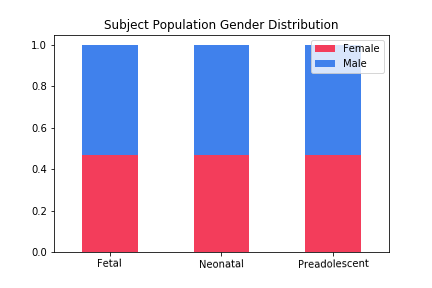
\includegraphics[width=.75\textwidth]{5/demo_clinical_subj_gender.png}
\caption{Distribution of subject genders for all three cohorts.}
\label{ch5:clinical:gender}
\end{figure}

\subsubsection{Neonatal Cohort and Images}

Neonatal subjects have been recruited as part of a prospective observational study. This cohort was scanned at two sites. At Site 1, the subjects were scanned using either a 3T Skyra (Siemans AG, Erlangen, Germany) or a 3T GE . At Site 2, the subjects were scanned using a 3T Philips (*).

The subjects were unsedated during the scans and a ``feed and bundle'' protocol was used to prevent motion during the scans \cite{Windram2011}. The newborns were positioned in the coil to minimize head tilting. Newborns were fitted with earplugs (Quiet Earplugs; Sperian Hearing Protection, San Diego, CA) and neonatal ear muffs (MiniMuffs; Natus, San Carlos, CA). An MR-compatible vital signs monitoring system (Veris, MEDRAD, Inc. Indianola, PA) was used to monitor neonatal vital signs. All scans were performed using a multi-channel head coil. The parameters for the resting-state BOLD MR scans were FOV=240 mm and TE/TR=32/2020 ms with interplane resolution of 4x4 mm, slice thickness of 4 mm, and 4 mm space between slices. The acquired images contained 150 volumes where each volume consisted of 64x64x32 voxels$^3$.

\begin{figure}
\centering
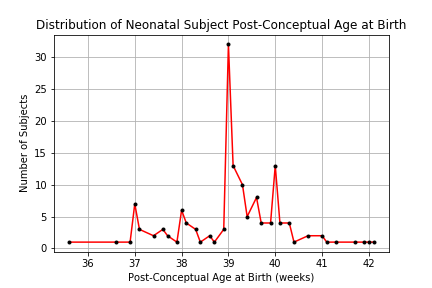
\includegraphics[width=.75\textwidth]{5/demo_neonate_subj_pca.png}
\caption{The distribution of post-conceptual ages at birth of all neonatal subjects.}
\label{ch5:neonates:birthpca}
\end{figure}

\begin{figure}
\centering
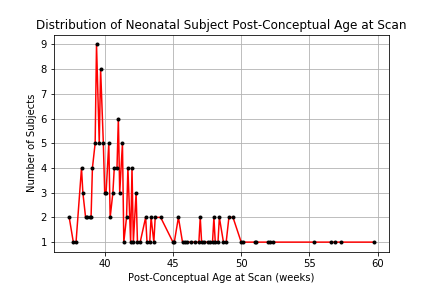
\includegraphics[width=.75\textwidth]{5/demo_neonate_scan_pca.png}
\caption{The distribution of post-conceptual ages at the time of the scan of all neonatal subjects.}
\label{ch5:neonates:scanpca}
\end{figure}

A total of 149 patients were recruited. The average post-conceptual age of the patients at birth was 39.08 weeks and they were on average 42.64 weeks post-conception at the time of the scan. The distribution of post-conceptual ages of the subjects at birth and at the time of the scan can be seen in Figure \ref{ch5:neonates:birthpca} and Figure \ref{ch5:neonates:scanpca}. 

\begin{figure}
\centering
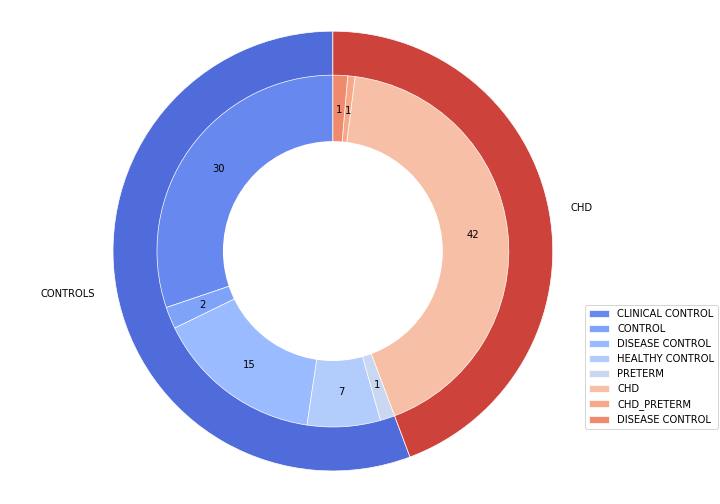
\includegraphics[width=1.0\textwidth]{5/demo_neonate_subj_cohort.png}
\caption{The breakdown of subject groups contained in the Control and CHD neonatal cohorts.}
\label{ch5:neonates:cohorts}
\end{figure}

The subjects were a mix of control subjects and CHD subjects. A comprehensive breakdown description of the subgroups within these two cohorts can be seen in Figure \ref{ch5:neonates:cohorts}. In this figure, the term ``Control'' encompasses both healthy full-term subjects, healthy pre-term subjects, and non-CHD clinical subjects (clinical control and disease control). The CHD group is composed of subjects diagnosed with CHD who were either born full-term or pre-term. Of the entire cohort, 14 subjects underwent two scanning sessions resulting in 163 rs-fMRI scans.

As the neonates were most often asleep during the scan, they exhibit less motion overall compared to our other clinical cohorts. The high-motion neonates are an obvious exception to this concept, but many of the high-motion images contained long periods where the subject was stationary. Applying both the DAG-based framework and the traditional registration framework to these images provided the opportunity to compare the performances of both registration frameworks to each other in the context of the usability gold standard thresholds. 

\subsubsection{Preadolescent Subject Population and Images}

As part of a multicenter study of CHD in preadolescents, we collected rs-fMRIs from nine sites throughout the United States. These images were of patients in the age range of 9 to 13 years who either had CHD or were healthy with no neurocognitive impairments. In addition to the MRI scans, subjects who participated in this study were asked to participate in additional testing  either to determine their neurocognitive outcome status or to perform genetic analyses. % (GET DETAILS FROM NANCY).

\textbf{Preadolescent Cohort.} The multicenter imaging study of preadolescent subjects provides a unique opportunity to evaluate the efficacy of the DAG-based framework on a large subject cohort containing variable amounts of motion. The outcome of this experiment will be used in the next experiment to determine if there are any site-specific or vendor-specific variables influencing patient motion.

%\begin{itemize}
%\item How were the images gathered?
%\item How were the patients recruited?
%\item What are the imaging protocol details?
%\item What other information was collected?
%\end{itemize}

\subsubsection{Fetal Subject Population and Images}

%Real goal is to develop a method of registering fetal brain and placental images so that we can further examine the relationship between placental oxygen levels and fetal brain development. Longitudinally, this technique can be used to determine how placental oxygen flow and fetal brain development impact a patient over the course of his or her life. Once the relationship between the placenta and fetal brain development is better understood, we can determine a set of neuroprotective interventions to employ for at-risk patients before they are born.

Fetal subjects have different constraints on their physical environment than neonates, preadolescents, and adults. As a result, they exhibit unique patterns of motion. The previous subject cohorts discussed in this chapter have the following commonalities: the subject experiences the full effects of gravity, the subject is lying on his back in an MRI scanner, and the subject's head motion is limited by the head coil within the MRI. Any motion in these images is a direct result of the subject himself moving, whether passively (cardiac motion and breathing) or actively (fidgeting or looking around).

A fetal subject is scanned in vivo. He is suspended in amniotic fluid within his mother. The amniotic fluid has buoyancy that reduces the effects of gravity and allows a fetal subject significant freedom of movement. The fetus can rotate, shift, and flip in ways that can only be accomplished when floating in a body of water. The properties of the uterus constrain the physical space in which a motion could occur, but not as much as the head coil and gravity do to the other patient cohorts. A fetus is not guaranteed to be in any specific position at the start of the scan: the scan begins when the mother is ready, not when the fetus achieves a certain pose. 

The fetal subjects underwent fetal echocardiography scans in a cardiac clinic to determine whether they were healthy or had a form of CHD. They were then scanned on an MRI scanner. Images of the fetal brain and the placenta were acquired for each subject. 

We are interested in both the fetal brain and placental images for our work because of the relationship between placenta and brain development. However, these organs have very different physical properties. The fetal brain is a rigid structure floating and moving within the amneotic fluid. It undergoes translation and rotation as a single unit due to passive and active maternal and fetal motions. The placenta, on the other hand, is anchored in place on the uterine wall. It may undergo small translations or rotations due to maternal motion, but it will respond differently to fetal motion. Fetal motions cause nonlinear deformations of the pliable placenta that can only be adequately accounted for using nonlinear registration algorithms. Nonlinear registrations have the potential to deform brain images into physically impossible shapes, so the fetal brain and placenta were manually segmented in their respective images so that each organ could undergo independent motion correction. 

The segmenters were one of a group of four researchers. While one researcher trained the other three group members, the interrater agreement between them is still being determined.

As the fetal subjects have both neurological and placental images, their data will be used to examine the impact of volume registration on different organ types.


%\begin{itemize}
%\item Fetal patients scanned between XX and XX weeks gestational age. 
%\item Imaging protocol details?
%\item What other information is collected about fetus and/or mom?
%\end{itemize}

\subsubsection{Aging Brain Subjects}

The ADNI study was launched in 2003 as a public-private partnership, led by Principal Investigator Michael W. Weiner, MD. The primary goal of ADNI has been to test whether serial magnetic resonance imaging (MRI), positron emission tomography (PET), other biological markers, and clinical and neuropsychological assessment can be combined to measure the progression of mild cognitive impairment (MCI) and early Alzheimer's disease (AD). For up-to-date information, see www.adni-info.org.

%\begin{itemize}
%\item How were the images gathered?
%\item How were the patients recruited?
%\item What are the imaging protocol details?
%\item What other information was collected?
%\end{itemize}

%The second adult cohort comes from the Alzheimer's Disease Neuroimaging Initiative (ADNI) dataset. The ADNI study has been working since 2004 to further Alzheimer's research by gathering, analyzing, and sharing clinical, imaging, genetic, and biochemical biomarkers from the elderly population. The group gathers data from 63 sites in the United States and Canada. During the second phase of the study, sites who have a Philips MRI system gathered resting-state fMRIs from their subjects. This data is freely available to academic researchers through the LONI Image and Data Archive.

The adult cohort encompass many clinical outcomes and a wider age range than the other clinical populations. The adult cohort also allows for another opportunity to study a different type of motion patterns associated with the aging brain rather than the still-developing brain.

\subsection{Summary}
%ELEPHANTS 3-5 sentences about CHD here

While we have amassed a large collection of clinical images, an analysis of purely clinical images is not sufficient in determining which volume registration technique recovers more brain signal. In the next section, we elaborate on this limitation and how we chose to address it.

\section{Simulated Sequences} % ELEPHANTS should this be its own chapter?

There are two major barriers in research surrounding motion correction in rs-fMRIs: gathering data and measuring the effects of the technique. In this section, we elaborate on a simulation designed to address both of these barriers.

\subsection{Background}

Despite the hundreds of images in each of the patient populations described in the previous section, our clinical data would be considered too sparse for ``big data'' analyses. This problem is not unique to our group: it is difficult to obtain enough data from a large number of subjects to perform large-scale studies. Collaborators can band together to create a larger and more diverse data set by participating in multicenter studies. There are some challenges associated with multicenter studies. Each site will have a different scanner, potentially with different field strengths and from different manufacturers. Even ignoring the challenges of harmonizing data obtained using scanners from different companies, each scanner has its own set of unique inhomogeneities in the primary magnetic field. Additional scans of inanimate or human phantoms may be necessary to characterize the differences between all of the scanners involved.

The second barrier to motion correction in rs-fMRI research is the complexity of identifying a gold standard metric to use when evaluating motion correction techniques. The current gold standard metrics developed by Power et al. evaluate motion correction techniques in terms of the reduction of positional differences and signal differences between neighboring volumes. Unfortunately, this approach does not measure the amount of signal recovered or lost though motion correction. A true gold standard evaluation of motion correction would be able to evaluate the BOLD signal present in the image before and after correction. If the BOLD signal prior to patient motion was known, though, there would be no need for image processing in the first place: we would already have the data we are trying to obtain with motion correction.

We address these two barriers by creating a mechanism for generating simulated image sequences. The generated sequences contain simulated brain signal based in areas of the brain associated with resting-state connectivity, scanner noise, and patient motion. Our mechanism can create large quantities of unique image sequences. The simulated image sequences can also serve as a gold standard for evaluating volume registration and motion correction techniques: the signals and noise sources added to the sequence are known with certainty.

%Every MRI scanner is different, even those made by the same manufacturer. To ensure MRI scans obtained from different scanners are comparable.  so a stand-in model for an organ or tissue type is often used to calibrate an MRI scanner. The model is designed to have specific physical properties which mimic the physical properties of the organ or tissue. These properties can be accurately measured during the design process of this model so that the radiologist or researcher looking at images of the model can know the ground truth of the model. Because these models mimic true organs and tissues, they are called phantoms. 

\subsection{SPECTr: Simulated Phantom Emulating Cranial Transformations}

Our mechanism is called Simulated Phantom Emulating Cranial Transformations (SPECTr). A phantom is an object designed to have material properties which mimic those of a specific tissue type or organ. Phantoms, either manufactured objects or healthy humans, are used in multicenter studies to obtain images of the same object or person from multiple scanners. These images are used to harmonize the data taken from the different sites. We call our simulated sequence a phantom because the baseline image itself is known as are the signals added to it to simulate brain activity. 

% ELEPHANTS
When developing the pipeline for SPECTr, it was important to consider the effects of motion and various impacts they have on the BOLD signal. As discussed in CHAPTER, the three effects of motion are positional, spin history, and susceptibility. For simplicity, we combine the spin history and susceptibility effects into ...

\subsection{Materials}

In order to simulate resting-state BOLD signal in an fMRI, two pieces of anatomical information are required. The first is structural information about the brain. The second is the location of functional networks associated with the resting-state BOLD signal.

While it is possible to use clinical images for the structural information, the goal of SPECTr is to be generalizable both for our use and for the use of other researchers. Additionally, clinical images inherently contain some degree of signal from some neuronal processes which could obfuscate the simulated BOLD signal. 

In 1992, the International Consortium for Brain Mapping was formed to develop as set of standards for what is considered a healthy human brain. They used their criteria to develop an initial set of ``average'' brain structural scans based on scans from healthy volunteers. This original set of average brain scans incorporates scans from 305 subjects and is referred to as the MNI305 data. As MRI technology has evolved, the spatial resolution capabilities of the MRI scanners has increased. In 2001, another set of 152 healthy volunteers was recruited to create a higher resolution data set. The scans from the new cohort were linearly registered to the MNI305 data to create the new MNI152 images. % ELEPHANTS citations needed

Herein, we use the MNI152 data set as available at the website for the McConnell Brain Imaging Centre at McGill University. This data set contains five images: a T1-weighted scan, a T2-weighted scan, a proton density weighted scan, and two binary masks for the head and the brain. Each of the structural scans was designed to highlight the properties of different tissues in and around the brain. Proton density scans were developed for the purpose of detecting blood-related signal. As BOLD images essentially perform the same purpose over a period of minutes, we choose to use the proton density weighted scan as the structural base for the simulated images. % ELEPHANTS citations needed

The functional network information is more difficult to find than structural atlases. The Functional Imaging in Neuropsychiatric Disorders Lab at Stanford has developed two sets of functional atlases. The atlases are divided into regions of interest (ROIs) associated with individual networks. The first set of atlases contains 90 functional ROIs which compose 14 networks. The second set of atlases contains 499 functional ROIs and has more gray matter coverage. For simplicity, we chose to use the original ROIs associated with the dorsal and ventral default mode networks.

\subsection{Simulation Pipeline}

\subsubsection{Baseline Sequence}

\begin{figure}
\centering

\includegraphics[width=.5\textwidth]{5/pipeline.png}
\caption{An overview of the SPECTr simulation pipeline. Using atlas data, a simulated phantom containing brain signal, scanner noise, and patient motion is generated.}
\label{ch5:spectr_flow}
\end{figure}

The process for generating a simulated sequence using the data discussed in the previous section has several steps. An overview of the pipeline can be seen in Figure \ref{ch5:spectr_flow} We cover these steps in detail in this section.

The MNI152 proton density image is a whole head image. To remove the skull, we apply the brain mask to the proton density weighted image. The resulting image contains only brain tissue.

The spatial resolution of the structural brain image is 1 mm$^3$. The spatial resolution for a single volume in a rs-fMRI sequence is less granular at 4mm$^3$. To achieve this resolution, the structural volume must be downsampled. After the downsampling, the size of the structural image is reduced from 181x217x181 voxels to XXxXXxXX voxels. %ELEPHANTS interpolation?

Now that the structural image is the correct spatial resolution, it must be replicated to create the temporal sequence. Part of this step includes creating a new dimension in the data. The affine matrix which represents the resolution of the image has the following structure:

\begin{equation}
\begin{bmatrix}
 r_x &  0   &  0   & c_x\\ 
 0   &  r_y &  0   & c_y \\ 
 0   &  0   &  r_z & c_z \\ 
 0   &  0   &  0   & 1 
\end{bmatrix}
\end{equation}

\noindent where $r_x, r_y,$ and $r_z$ represent the spatial resolution in the $x, y,$ and $z$ axes, respectively and $c_x, c_y,$ and $c_z$ represent the location of the origin in voxels. To convert the image from a 3D volume to a 4D sequence, we add a row and a column to this matrix so that it now has the structure:

\begin{equation}
\begin{bmatrix}
 r_x &  0   &  0   & 0 & c_x\\ 
 0   &  r_y &  0   & 0 & c_y \\ 
 0   &  0   &  r_z & 0 & c_z \\ 
 0   &  0   &  0   & t & 0 \\
 0   &  0   &  0   & 0 & 1 
\end{bmatrix}
\end{equation}

\noindent where $t$ is the desired temporal resolution. We choose a temporal resolution of 2 seconds for our simulated sequence. The downsampled image volume is replicated and concatenated along the new temporal dimension to create a sequence that is 150 image volumes long. This sequence is referred to as the base phantom sequence as it contains no brain signal, noise, or motion.

\subsubsection{Brain Signal}

The next step in the pipeline is to add BOLD signal to the sequence. % ELEPHANTS (Why brain signal next?) 
We combine the functional ROIs from the dorsal and ventral default mode networks into a single binary functional ROI image. This image is referred to as the default mode network (DMN) mask. 

For each nonzero voxel in the DMN mask, a temporal signal is generated. We chose to model the BOLD response as a cosine signal following the formula

\begin{equation}
s(\vec{v}, t) = a*(cos(f_0 * (t-t_{shift})) - a_shift).
\label{ch5:bold_eq}
\end{equation}

\noindent This equation is for a scaled cosine function with both temporal and amplitude shifts. The temporal and amplitude shifts, $t_{shift}$ and $a_{shift}$ respectively, are randomly generated for each voxel from uniform distributions. Once chosen, they are consistent across the voxel's generated temporal signal. The other parameters, $a$ and $f_0$, were specified using existing research. 

In 2007, Biswal et al. performed a study evaluating methods to reduce changes in the BOLD signal not directly related to brain activity (i.e., vascularity). They identified a low-frequency spectral amplitude of 0.04 Hz as the highest frequency related to BOLD signal consistent not only through scans of individual patients but in group-wise analyses. Based on their work, we chose the fundamental frequency $f_0$ to be 0.04 Hz. % ELEPHANTS citation

The scaling factor $a$ was chosen based on Power et al.'s usability criteria. As they state that any signal change between volumes above 2.5\% of the maximum voxel value is unlikely to be due to brain activity, we used an amplitude of 20 units on a scaled voxel value range of [0, 1000]. % ELEPHANTS citation

The generated BOLD signals were added to the baseline image sequence, but were also saved in a separate image sequence file for reference during analysis. The generated sequence with only BOLD signal is referred to as the brain signal sequence.

\subsubsection{Scanner Noise}

The next step in the pipeline is to add scanner noise to the brain signal sequence. In a regular rs-fMRI of a patient, the noise in the sequence is the result of two factors: the spin history effects of motion and the susceptibility effects of motion. To simplify the simulation, we choose to model the resulting noise rather than the individual sources.

Signal acquired by MRI scanners is first recorded as a raw data matrix in k-space. K-space contains spatial frequency information. The coordinate system of k-space differs from the coordinate system of physical space. In k-space, the closer a point is to the center of a zero-centered data matrix, the lower its frequency or phase. The brighter a point in the raw data matrix is, the larger its magnitude. 

While frequency is a continuous spectrum, data is usually divided into low frequency data and high frequency data. Low frequency data in imaging is areas of an image where the pixel or voxel values slowly. In physical space, these areas are the smooth areas that contain content. In Figure REF, the skin on the woman's face would be considered low frequency data. High frequency data represents the areas in an image where the pixel or voxel values change rapidly in a small area. Areas with many edges in them contain higher frequency data. In Figure REF, the feather in the woman's hat would be considered high frequency data. % Need a figure ELEPHANTS 

Generally speaking, images contain more low frequency information than high frequency information. We wish to be able to control the amount of noise added to each component independently, so we choose to add noise to the sequence in k-space.

When adding scanner noise to the brain signal sequence, we add noise to each image volume independently. The image volume is transformed from physical space into k-space using the fast Fourier transform (FFT). To force the image to be zero-centered, we perform a FFT shift on the Fourier space data. A matrix the same size and shape as the image volume is created. The matrix is then filled with complex Gaussian noise, $n(\vec{l})$ where

\begin{equation}
|n(\vec{l})| = w_m * r_m, r_m~N(0,1)
\end{equation}

\noindent and

\begin{equation}
\angle n(\vec{l}) = w_p * r_p, r_p~N(0,1)
\end{equation}

\noindent In these two equation, $\vec{l}$ is the location of the point in the matrix, $w_*$ represents the weight assigned to the component, $r_*$ represents the noise random variable independently generated from a standard normal distribution, and the subscripts $m$ and $p$ refer to the magnitude and phase components, respectively. The complex noise is weighted so that the magnitude of the noise has a greater contribution than the phase of the noise, that is $w_m > w_p$ 

The matrix of complex noise is added to the zero-centered k-space image volume. The noisy k-space volume is unshifted and undergoes an inverse Fourier transform to change the data back to physical space.

\subsubsection{Patient Movement}

Now that the ground truth brain orientation and BOLD signal have been established, patient motion can be added to the BOLD phantom sequence. One of the aims of this document is to establish that patients from different populations exhibit different motion patterns. As we have not yet established what those motion patterns are, we developed a generic motion model for the simulation.

During an rs-fMRI scan, a patient theoretically has the freedom to rotate his head around three different axes, translate his head along three different axes, or some combination of translations and rotations. Realistically, once a patient has settled in the scanner, it becomes difficult for his head to only undergo translation. It is more likely that he will rotate his head. For the simplicity of the simulation, we assume no head translations occur during the scan.

A rotational transformation can be represented as a matrix. Rotations about a single axis are represented as followed:

\begin{equation}
R_x(\alpha) = \begin{bmatrix}
 1 &  0          & 0     \\ 
 0 &  cos\alpha  & sin\alpha \\ 
 0 &  -sin\alpha & cos\alpha \\ 
\end{bmatrix}
\end{equation}
\begin{equation}
R_y(\beta) = \begin{bmatrix}
 cos\beta &  0 & -sin\beta \\ 
 0        &  1 & 0         \\ 
 sin\beta &  0 & cos\beta  \\ 
\end{bmatrix}
\end{equation}
\begin{equation}
R_z(\gamma) = \begin{bmatrix}
 cos\gamma  & sin\gamma  & 0 \\ 
 -sin\gamma & cos\gamma  & 0 \\ 
 0          & 0          & 1 \\ 
\end{bmatrix}
\end{equation}

Rotational transforms are applied to the origin of the image. However, the origin of the image is not necessary anatomically significant. Head motion naturally occurs about the base of the neck. We can approximate the location of the base of the neck by calculating the center of mass of the brain. First, the image volume is thresholded to separate the brain from the background. Then the locations of the ``on'' voxels are averaged to calculate the center of mass. 

Motion is added to the noisy image sequence one volume at a time. No motion is applied to the first volume in the sequence, but volume is used to calculate the center of mass of the brain. For each subsequent volume, the angles of rotation about the x-, y-, and z-axes are each randomly generated from a standard normal distribution to create rotational change matrices, $R_{*,\Delta}$ (where the subscript $*$ represents $x$, $y$, or $z$). The new rotations $R_{*,\Delta}$ are added to the rotations from the previous step $R_{*,i-1}$ to create the rotation matrices for the current volume, $R_{*,i}$:

\begin{equation}
R_{*,i} = R_{*,i-1} + R_{*,\Delta}
\end{equation}

The three rotational transformations are combined into one matrix via multiplication: 

\begin{equation}
R_i = R_{x, i}(\alpha) R_{y,i}(\beta) R_{z,i}(\gamma)
\end{equation}

The compound transformation $R_i$ is then applied to the image at the center of mass calculated from the original image volume. \textit{Note: Since the simulation is constrained by the assumption of no head translations, the center of mass will remain consistent throughout the image sequence.}

After motion has been added to every image volume in the sequence, the sequence with motion is ready to be used in motion correction analyses.

\subsection{Implementation}

SPECTr is implemented in Python (version 3.7.3). The \lstinline{nipy} library (version 0.4.1) was used to load images, save images, and combine the functional ROIs. The \lstinline{numpy} library (version 1.17.4) was used for matrix manipulations involved in the brain signal and noise generation steps. The image processing library \lstinline{skimage} (version 0.14.2) was used to calculate the center of mass. The Python wrapper \lstinline{SimpleITK} (version 1.2.4) of the Insight Toolkit library for image analysis was used to perform the rotational transformations associated with patient motion.

The source code for SPECTr is available on Github at \url{https://github.com/jmschabdach/SPECTr}.


%First, a reasonable range of head rotation about the x-, y-, and z-axes was established. These angle ranges are used to generate rotational transformation matrices for $N-1$ image volumes. The transformations are applied to each image volume after the first volume in the BOLD phantom sequence. The transformed image sequence is referred to as the BOLD phantom sequence with motion and the rotational transformation matrices are saved as the ground truth for the transformations between each image volume and the template volume. 
%The BOLD phantom sequence serves as the ground truth for any motion correction pipeline: it contains the known brain orientation and BOLD signal independent from head motion and scanner noise.

\subsection{Experiments Involving Simulated Images}

We generated 90 image sequences from the MNI152 proton density image and the default mode network functional ROIs using the process described in the previous section. The image sequences were divided into three groups with different degrees of scanner noise. All simulated images underwent both registration techniques described in Chapter \ref{ch:mri}. The registered images also underwent independent component analysis (ICA) using FSL's MELODIC (Multivariate Exploratory Linear Optimized Decomposition into Independent Components) tool. % ELEPHANTS SOURCES

The registered images will undergo the same type of analysis as the clinical images. The ICA technique will be used to determine how much brain signal was recovered by each registration technique.

This particular experiment will be one of the first to investigate how much true BOLD signal is preserved through motion correction. One of the major drawbacks to existing motion correction pipelines is that they remove signal along with noise. In clinical data, there is no way to know the ground truth signal contained within the image; however, simulated phantom images have a de facto known ground truth signal. The design for this experiment can be used to evaluate how much BOLD signal is recovered by other motion correction pipelines, and how close the recovered signal is to the signal of interest.

\section{Summary}

In this chapter, we discussed our three major data sets, which are drawn from simulated data, pediatric data, and aging brain data. The simulated data were generated using a rs-fMRI simulation pipeline developed in-house and were used for the purpose of measuring ground truth signal recovered by motion correction techniques. The pediatric data were obtained through prospective studies of CHD and neurodevelopment being conducted at the UPMC Children's Hospital of Pittsburgh. The pediatric and aging brain images were used to compare the two volume registration techniques in a standalone analysis as well as in the context of a motion correction pipeline. We also used these images to examine patterns of motion unique to different age groups. 

% FIX CONTENTS
\chapter{RESULTS}
\label{ch:results}

This chapter is divided into two main sections. The first section focuses on the comparison of the two motion correction techniques. The second section focuses on the results of the machine learning algorithms applied to the metrics extracted from the images.

Each of the clinical images underwent volume registration using both registration methods outlined in Chapter \ref{ch:moco}. The FD and DVARs metrics were calculated for every pair of subsequent volumes $i$ and $i+1$ in the original sequences, the traditionally registered sequences, and the DAG-registered sequences. Then the sequences were comprehensively compared to themselves. For every volume in each sequence, the Dice metric, the mutual information, and the correlation ratio were calculated for the volume and every other volume in the sequence.

The simulated data underwent the same analyses as the clinical images, with one addition. Independent component analysis was performed on the simulated data to identify components contributing to the overall signal in the image. By correlating the components with the simulated signal for each image, the BOLD-related components were identifies. The amount of BOLD signal identified for each image was compared to that image's original BOLD signal.


\section{Simulated Data}

\subsection{Volume Registration: Power Thresholds}

\begin{figure}[t]
	\centering
	\begin{subfigure}{0.4\textwidth}
		\centering
		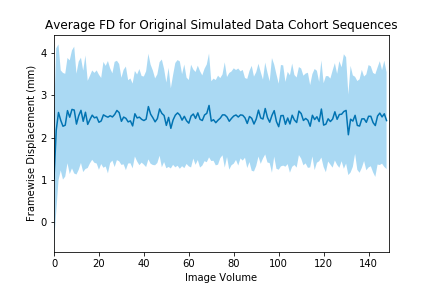
\includegraphics[width=1.0\textwidth]{6/figures/spectr-bold-fd-150.png}
		\caption{FD of Original Sequences.}
	\end{subfigure}
	\hspace{0.05\textwidth}
	\begin{subfigure}{0.4\textwidth}
		\centering
		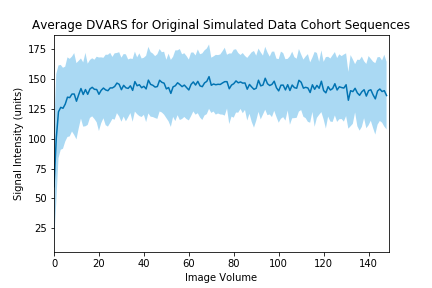
\includegraphics[width=1.0\textwidth]{6/figures/spectr-bold-dvars-150.png}
		\caption{DVARS of Original Sequences.}
	\end{subfigure}
	
	\begin{subfigure}{0.4\textwidth}
		\centering
		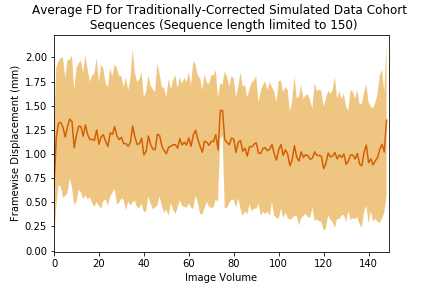
\includegraphics[width=1.0\textwidth]{6/figures/spectr-trad-fd-150.png}
		\caption{FD of Traditionally Registered Sequences.}
	\end{subfigure}
	\hspace{0.05\textwidth}
	\begin{subfigure}{0.4\textwidth}
		\centering
		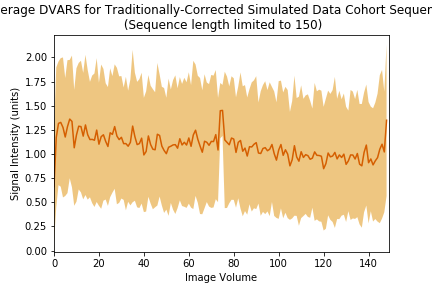
\includegraphics[width=1.0\textwidth]{6/figures/spectr-trad-dvars-150.png}
		\caption{DVARS of Traditionally Registered Sequences.}
	\end{subfigure}
	
	\begin{subfigure}{0.4\textwidth}
		\centering
		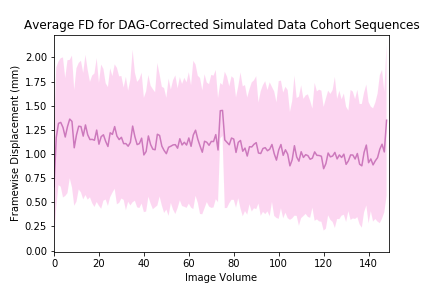
\includegraphics[width=1.0\textwidth]{6/figures/spectr-dag-fd-150.png}
		\caption{FD of DAG-Registered Sequences.}
	\end{subfigure}
	\hspace{0.05\textwidth}
	\begin{subfigure}{0.4\textwidth}
		\centering
		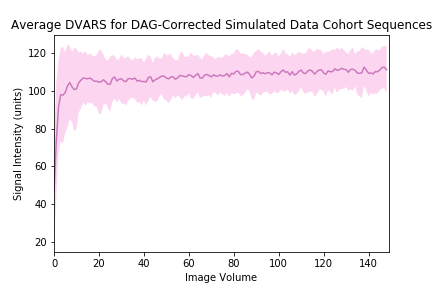
\includegraphics[width=1.0\textwidth]{6/figures/spectr-dag-dvars-150.png}
		\caption{DVARS of DAG-Registered Sequences.}
	\end{subfigure}
\caption{The means and standard deviations of the FD and DVARS metrics for all simulated images both before and after registration.}
\label{fig:neonate-power-dists}
\end{figure}

The FD and DVARS metrics were calculated between every pair of image volumes $i-1$ and $i$ for the original sequences and both types of registered sequences. The mean of the FD and DVARS metrics for each time point for each sequence type  can be seen in Figures

\begin{table}[h!]
\centering
\caption{The number and percentage of image volumes across all sequences in the simulated cohort which meet the usability thresholds of FD \textless 0.2 mm and DVARS \textless 2.5\%.}
\label{tab:spectr-power-thresh}
\begin{tabular}{|c|c|c|c|}
\hline
\textbf{Threshold Met} &
  \textbf{\begin{tabular}[c]{@{}c@{}}Original\\  Sequences\end{tabular}} &
  \textbf{\begin{tabular}[c]{@{}c@{}}Traditionally Registered \\ Sequences\end{tabular}} &
  \textbf{\begin{tabular}[c]{@{}c@{}}DAG-Registered \\ Sequences\end{tabular}} \\ \hline
FD (count)    & 98    & 329   & 279   \\ \hline
DVARS (count) & 54    & 53    & 53    \\ \hline
Both (count)  & 53    & 46    & 44    \\ \hline
FD (\%)       & 0.731 & 2.453 & 2.081 \\ \hline
DVARS(\%)     & 0.403 & 0.395 & 0.395 \\ \hline
Both (\%)     & 0.395 & 0.343 & 0.328 \\ \hline
\end{tabular}
\end{table}

Table \ref{tab:spectr-power-thresh} shows the number of and percentage of image volumes in all simulated image sequences which meet the FD threshold, the DVARS threshold, and both thresholds. Across all 90 image sequences, there were 150 image volumes per sequence bringing the total number of image volumes to 13,410 image volumes. In the original images, less than 1\% of the image volumes met the individual thresholds with only 0.395\% of image volumes meeting both thresholds. After either registration, over 2\% of the image volumes meet the FD threshold.

\begin{table}[h!]
\centering
\caption{Results from the t-tests comparing the counts for the numbers of images meeting the FD, DVARS, and FD and DVARS thresholds for sequence type $S_1$ and sequence type $S_2$.}
\label{tab:spectr-power-ttest}
\begin{tabular}{|c|c|c|c|}
\hline
\textbf{Sequence Type 1 ($S_1$)} &
  \textbf{Original} &
  \textbf{Original} &
  \textbf{\begin{tabular}[c]{@{}c@{}}Traditionally \\ Registered\end{tabular}} \\ \hline
\textbf{Sequence Type 2 ($S_2$)} &
  \textbf{\begin{tabular}[c]{@{}c@{}}Traditionally\\ Registered\end{tabular}} &
  \textbf{\begin{tabular}[c]{@{}c@{}}DAG\\ Registered\end{tabular}} &
  \textbf{\begin{tabular}[c]{@{}c@{}}DAG\\ Registered\end{tabular}} \\ \hline
\begin{tabular}[c]{@{}c@{}}P($S_1$ and $S_2$ have \\ same FD counts)\end{tabular} &
  1.05 E -16 &
  4.49 E -11 &
  0.127 \\ \hline
\begin{tabular}[c]{@{}c@{}}P($S_1$ and $S_2$ have \\ same DVARS counts)\end{tabular} &
  0.941 &
  0.941 &
  1.0 \\ \hline
\begin{tabular}[c]{@{}c@{}}P($S_1$ and $S_2$ have \\ same FD and DVARS counts)\end{tabular} &
  0.590 &
  0.486 &
  0.872 \\ \hline
\end{tabular}
\end{table}

To determine the statistical significance of these differences, a series of independent 2 sample t-tests were performed. For each test, two types of sequences were chosen. The distributions of samples were the numbers of image volumes in each sequence meeting the usability threshold of interest. The null hypotheses for the t-tests were that the number of volumes meeting the threshold for each sequence type were the same and the alternative hypothesis was that this number was different. The results of these tests can be seen in Table \ref{tab:spectr-power-ttest}. The only statistically significant differences were for the number of image volumes meeting the FD threshold. The counts for the registered images each differed from the original images at $p < 0.005$ while the difference between the two registrations was not significant ($p = 0.127$).

\begin{table}[h!]
\centering
\caption{The number of subjects whose sequences of types $S_1$ and $S_2$ had different FD distributions.}
\label{tab:spectr-fd-kstest}
\begin{tabular}{|c|c|c|c|}
\hline
\textbf{\begin{tabular}[c]{@{}c@{}}\# Sequences \\ Type 1 ($S_1$)\end{tabular}} &
  \textbf{\begin{tabular}[c]{@{}c@{}}\# Sequences \\ Type 2 ($S_2$)\end{tabular}} &
  \textbf{\begin{tabular}[c]{@{}c@{}}\# Sequences \\ p \textless 0.05\end{tabular}} &
  \textbf{\begin{tabular}[c]{@{}c@{}}\# Sequences \\ p \textless 0.005\end{tabular}} \\ \hline
Original                                                            & \begin{tabular}[c]{@{}c@{}}Traditionally\\ Registered\end{tabular} & 90 & 90 \\ \hline
Original                                                            & \begin{tabular}[c]{@{}c@{}}DAG\\ Registered\end{tabular}           & 90 & 90 \\ \hline
\begin{tabular}[c]{@{}c@{}}Traditionally \\ Registered\end{tabular} & \begin{tabular}[c]{@{}c@{}}DAG\\ Registered\end{tabular}           & 40 & 27 \\ \hline
\end{tabular}
\end{table}

\begin{table}[h!]
\centering
\caption{The number of subjects whose sequences of types $S_1$ and $S_2$ had different DVARS distributions.}
\label{tab:spectr-dvars-kstest}
\begin{tabular}{|c|c|c|c|}
\hline
\textbf{\begin{tabular}[c]{@{}c@{}}\# Sequences \\ Type 1 ($S_1$)\end{tabular}} &
  \textbf{\begin{tabular}[c]{@{}c@{}}\# Sequences \\ Type 2 ($S_2$)\end{tabular}} &
  \textbf{\begin{tabular}[c]{@{}c@{}}\# Sequences \\ p \textless 0.05\end{tabular}} &
  \textbf{\begin{tabular}[c]{@{}c@{}}\# Sequences \\ p \textless 0.005\end{tabular}} \\ \hline
Original                                                            & \begin{tabular}[c]{@{}c@{}}Traditionally\\ Registered\end{tabular} & 90 & 90 \\ \hline
Original                                                            & \begin{tabular}[c]{@{}c@{}}DAG\\ Registered\end{tabular}           & 90 & 90 \\ \hline
\begin{tabular}[c]{@{}c@{}}Traditionally \\ Registered\end{tabular} & \begin{tabular}[c]{@{}c@{}}DAG\\ Registered\end{tabular}           & 3  & 0  \\ \hline
\end{tabular}
\end{table}

For a more general comparison, the FD and DVARS metrics for each subject were compared for each type of registration. These distributions of FD and DVARS values for the original, traditionally registered and DAG-registered sequences underwent pairwise comparisons using the Kolmogorov-Smirnov test which evaluates the difference between two probability distributions. 

Table \ref{tab:spectr-fd-kstest} shows the number of comparisons between each sequence type where the Kolmogorov-Smirnov test produced a p-value less than 0.05 and 0.005 for the FD metrics. This table shows that the all images registered using either type of registration had significantly different FD distributions than the original images. It also shows that the traditionally registered and DAG-registered sequences had significantly different FD distributions with $p < 0.05$ for almost half (40/90) of the sequences and $p < 0.005$ for almost a third (27/90) of the sequences.

Table \ref{tab:spectr-dvars-kstest} shows similar results for the DVARS metrics of the registered and original sequences. However, only 3/90 of the registered image sequences had different DVARS distributions at $p < 0.05$. 



%Independent 2 sample t-test
%Null hypothesis: number of Traditional and DAG registered images meeting the FD threshold are the same
%Alternative hypothesis: number of traditional and dag registered images meeting the FD threshold are different
%Gather data: get number of images meeting each threshold from each sequence

\subsection{Volume Registration: Sequence Duration Motion}

\begin{figure}
\centering
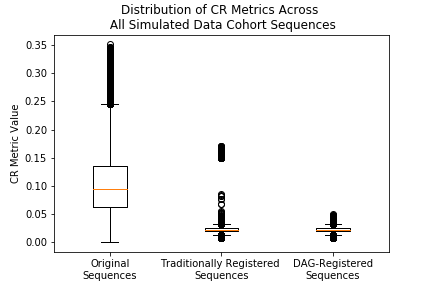
\includegraphics[width=0.5\textwidth]{6/figures/spectr-cr-box.png}
\caption{Boxplots of the values of all correlation ratio matrices for the original sequences, the traditionally registered sequences, and the DAG-registered sequences for the simulated data.}
\label{fig:spectr-cr-box}
\end{figure}

\begin{table}[]
\centering
\caption{Results of t-tests comparing the descriptive statistics of the correlation ratio matrices for the simulated data.}
\label{tab:spectr-cr-ttest}
\begin{tabular}{|c|c|c|c|}
\hline
\textbf{Sequence Type 1 ($S_1$)} &
  \textbf{Original} &
  \textbf{Original} &
  \textbf{\begin{tabular}[c]{@{}c@{}}Traditionally \\ Registered\end{tabular}} \\ \hline
\textbf{Sequence Type 2 ($S_2$)} &
  \textbf{\begin{tabular}[c]{@{}c@{}}Traditionally\\ Registered\end{tabular}} &
  \textbf{\begin{tabular}[c]{@{}c@{}}DAG\\ Registered\end{tabular}} &
  \textbf{\begin{tabular}[c]{@{}c@{}}DAG\\ Registered\end{tabular}} \\ \hline
\begin{tabular}[c]{@{}c@{}}P($S_1$ and $S_2$ \\ have same minimums)\end{tabular} &
  0.3487 &
  0.3407 &
  0.9821 \\ \hline
\begin{tabular}[c]{@{}c@{}}P($S_1$ and $S_2$ \\ have same 1st quartile)\end{tabular} &
  9.750 E -113 &
  1.246 E -112 &
  0.8019 \\ \hline
\begin{tabular}[c]{@{}c@{}}P($S_1$ and $S_2$ \\ have same medians)\end{tabular} &
  5.288 E -88 &
  5.409 E -88 &
  0.9997 \\ \hline
\begin{tabular}[c]{@{}c@{}}P($S_1$ and $S_2$ \\ have same 3rd quartiles)\end{tabular} &
  6.534 E -81 &
  6.730 E -81 &
  0.9577 \\ \hline
\begin{tabular}[c]{@{}c@{}}P($S_1$ and $S_2$ \\ have same maximums)\end{tabular} &
  2.536 E -98 &
  6.180 E -103 &
  0.4068 \\ \hline
\end{tabular}
\end{table}

\begin{figure}
\centering
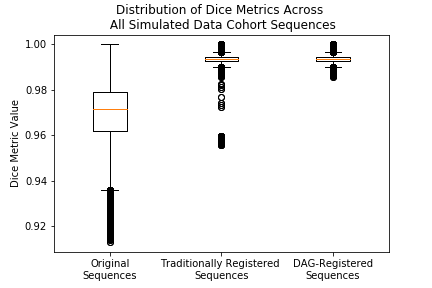
\includegraphics[width=0.5\textwidth]{6/figures/spectr-dice-box.png}
\caption{Boxplots of the values of all Dice matrices for the original sequences, the traditionally registered sequences, and the DAG-registered sequences for the simulated data.}
\label{fig:spectr-dice-box}
\end{figure}

\begin{table}[]
\centering
\caption{Results of t-tests comparing the descriptive statistics of the Dice matrices for the simulated data.}
\label{tab:spectr-dice-ttest}
\begin{tabular}{|c|c|c|c|}
\hline
\textbf{Sequence Type 1 ($S_1$)} &
  \textbf{Original} &
  \textbf{Original} &
  \textbf{\begin{tabular}[c]{@{}c@{}}Traditionally \\ Registered\end{tabular}} \\ \hline
\textbf{Sequence Type 2 ($S_2$)} &
  \textbf{\begin{tabular}[c]{@{}c@{}}Traditionally\\ Registered\end{tabular}} &
  \textbf{\begin{tabular}[c]{@{}c@{}}DAG\\ Registered\end{tabular}} &
  \textbf{\begin{tabular}[c]{@{}c@{}}DAG\\ Registered\end{tabular}} \\ \hline
\begin{tabular}[c]{@{}c@{}}P($S_1$ and $S_2$ \\ have same minimums)\end{tabular} &
  9.976 E -105 &
  2.520 E -110 &
  0.3778 \\ \hline
\begin{tabular}[c]{@{}c@{}}P($S_1$ and $S_2$ \\ have same 1st quartile)\end{tabular} &
  5.225 E -93 &
  5.582 E -93 &
  0.931 \\ \hline
\begin{tabular}[c]{@{}c@{}}P($S_1$ and $S_2$ \\ have same medians)\end{tabular} &
  1.988 E -104 &
  2.158 E -104 &
  0.9578 \\ \hline
\begin{tabular}[c]{@{}c@{}}P($S_1$ and $S_2$ \\ have same 3rd quartiles)\end{tabular} &
  1.679 E -131 &
  2.190 E -131 &
  0.842 \\ \hline
\begin{tabular}[c]{@{}c@{}}P($S_1$ and $S_2$ \\ have same maximums)\end{tabular} &
  1.0 &
  1.0 &
  1.0 \\ \hline
\end{tabular}
\end{table}

\begin{figure}
\centering
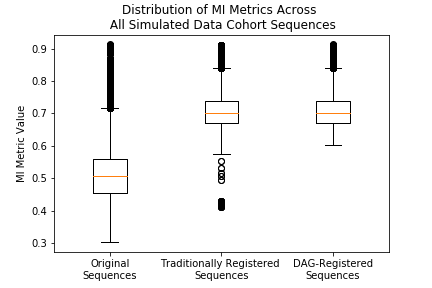
\includegraphics[width=0.5\textwidth]{6/figures/spectr-mi-box.png}
\caption{Boxplots of the values of all mutual information matrices for the original sequences, the traditionally registered sequences, and the DAG-registered sequences for the simulated data.}
\label{fig:spectr-mi-box}
\end{figure}

\begin{table}[]
\centering
\caption{Results of t-tests comparing the descriptive statistics of the MI matrices for the simulated data.}
\label{tab:spectr-mi-ttest}
\begin{tabular}{|c|c|c|c|}
\hline
\textbf{Sequence Type 1 ($S_1$)} &
  \textbf{Original} &
  \textbf{Original} &
  \textbf{\begin{tabular}[c]{@{}c@{}}Traditionally \\ Registered\end{tabular}} \\ \hline
\textbf{Sequence Type 2 ($S_2$)} &
  \textbf{\begin{tabular}[c]{@{}c@{}}Traditionally\\ Registered\end{tabular}} &
  \textbf{\begin{tabular}[c]{@{}c@{}}DAG\\ Registered\end{tabular}} &
  \textbf{\begin{tabular}[c]{@{}c@{}}DAG\\ Registered\end{tabular}} \\ \hline
\begin{tabular}[c]{@{}c@{}}P($S_1$ and $S_2$ \\ have same minimums)\end{tabular} &
  5.016 E -114 &
  6.328 E -126 &
  0.5397 \\ \hline
\begin{tabular}[c]{@{}c@{}}P($S_1$ and $S_2$ \\ have same 1st quartile)\end{tabular} &
  4.68 E -105 &
  7.90 E -105 &
  0.995 \\ \hline
\begin{tabular}[c]{@{}c@{}}P($S_1$ and $S_2$ \\ have same medians)\end{tabular} &
  1.65 E -97 &
  3.57 E -97 &
  0.994 \\ \hline
\begin{tabular}[c]{@{}c@{}}P($S_1$ and $S_2$ \\ have same 3rd quartiles)\end{tabular} &
  1.065 E -84 &
  2.374 E -84 &
  0.974 \\ \hline
\begin{tabular}[c]{@{}c@{}}P($S_1$ and $S_2$ \\ have same maximums)\end{tabular} &
  0.00473 &
  0.00794 &
  0.8761 \\ \hline
\end{tabular}
\end{table}

Motion across the whole sequence was measured by comparing every image volume in the sequence to every other image volume in the sequence. The three metrics used for this comparison were the correlation ratio, the Dice metric, and the mutual information metric. The calculations for a single metric on one sequence produced a two dimensional matrix of metric values. 

These matrices were used to compare the quantities of motion over the course of an entire sequence. For a population level comparison, the minimum, first quartile, median, third quartile, and maximum values of each matrix were computed for each sequence. The distribution of these values for sequences of one sequence type were compared to the distributions for a second sequence type using t-tests. The p-values that each metric comes from a different distribution can be seen in Table \ref{tab:spectr-cr-ttest} for the correlation ratio matrices, Table \ref{tab:spectr-dice-ttest} for the Dice matrices, and Table \ref{tab:spectr-mi-ttest} for the MI matrices. 

More generally, all matrix values for each sequence type were compared using the Kolmogorov-Smirnov test. The distributions for the correlation ratio metrics for the original, the traditionally registered, and the DAG-registered sequences differed at p < 0.005. The distributions for the Dice metrics and the mutual information metrics were also found to be from different distributions for each sequence type at p < 0.005. 

Figures HMM show boxplots of the distributions of each metric over the three sequence types. 

For the first analysis, the metrics matrices were compared to each other 

To compare motion patterns, the metrics matrices were normalized for each subject.


The differences in the motion patterns embodied by the normalized matrices were different between the original, traditionally registered, and DAG-registered sequences for each simulated subject was significant at $p < 0.005$.

Use t-test to compare the normalized matrices for all simulated subjects across a single registration type. Plot a clustermap based on 2 coordinates and the distance (p-value) between them

\subsection{*Volume Registration: Recovered Signal}


\section{Preadolescent Cohort}

\subsection{Volume Registration: Power Thresholds}

\begin{figure}[t]
	\centering
	\begin{subfigure}{0.4\textwidth}
		\centering
		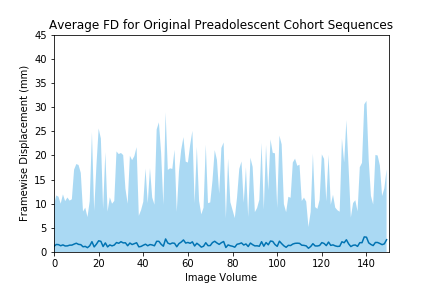
\includegraphics[width=1.0\textwidth]{6/figures/preads-bold-fd-150.png}
		\caption{FD of Original Sequences.}
	\end{subfigure}
	\hspace{0.05\textwidth}
	\begin{subfigure}{0.4\textwidth}
		\centering
		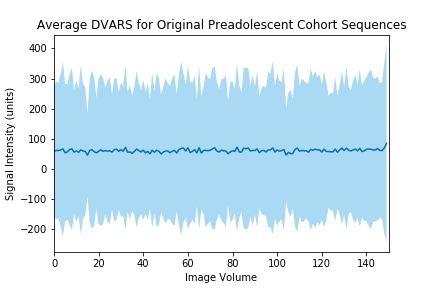
\includegraphics[width=1.0\textwidth]{6/figures/preads-bold-dvars-150.png}
		\caption{DVARS of Original Sequences.}
	\end{subfigure}
	
	\begin{subfigure}{0.4\textwidth}
		\centering
		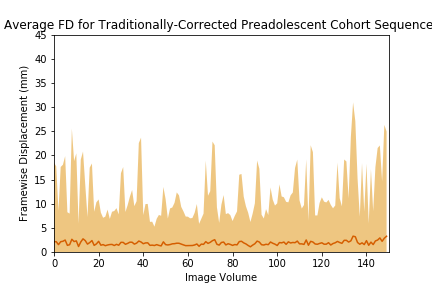
\includegraphics[width=1.0\textwidth]{6/figures/preads-trad-fd-150.png}
		\caption{FD of Traditionally Registered Sequences.}
	\end{subfigure}
	\hspace{0.05\textwidth}
	\begin{subfigure}{0.4\textwidth}
		\centering
		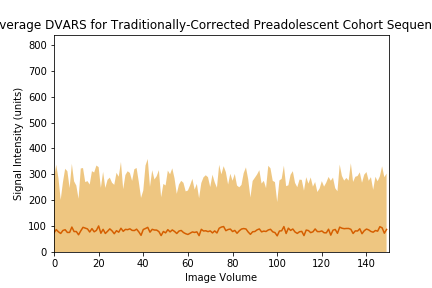
\includegraphics[width=1.0\textwidth]{6/figures/preads-trad-dvars-150.png}
		\caption{DVARS of Traditionally Registered Sequences.}
	\end{subfigure}
	
	\begin{subfigure}{0.4\textwidth}
		\centering
		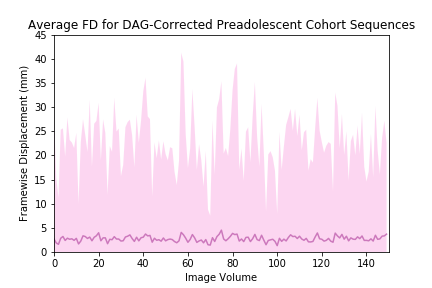
\includegraphics[width=1.0\textwidth]{6/figures/preads-dag-fd-150.png}
		\caption{FD of DAG-Registered Sequences.}
	\end{subfigure}
	\hspace{0.05\textwidth}
	\begin{subfigure}{0.4\textwidth}
		\centering
		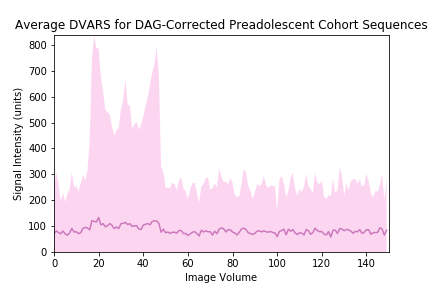
\includegraphics[width=1.0\textwidth]{6/figures/preads-dag-dvars-150.png}
		\caption{DVARS of DAG-Registered Sequences.}
	\end{subfigure}
\caption{The means and standard deviations of the FD and DVARS metrics for all preadolescent images both before and after registration.}
\label{fig:pread-power-dists}
\end{figure}

\begin{table}[h!]
\centering
\caption{The number and percentage of image volumes across all sequences in the preadolescent cohort which meet the usability thresholds of FD \textless 0.2 mm and DVARS \textless 2.5\%.}
\label{tab:pread-power-thresh}
\begin{tabular}{|c|c|c|c|}
\hline
\textbf{Threshold Met} &
  \textbf{\begin{tabular}[c]{@{}c@{}}Original\\  Sequences\end{tabular}} &
  \textbf{\begin{tabular}[c]{@{}c@{}}Traditionally Registered \\ Sequences\end{tabular}} &
  \textbf{\begin{tabular}[c]{@{}c@{}}DAG-Registered \\ Sequences\end{tabular}} \\ \hline
FD (count)    & 107879 & 72104 & 72114 \\ \hline
DVARS (count) & 87169  & 54056 & 53756 \\ \hline
Both (count)  & 74107  & 45006 & 44682 \\ \hline
FD (\%)       & 60.17  & 40.22 & 40.26 \\ \hline
DVARS(\%)     & 48.62  & 30.15 & 30.01 \\ \hline
Both (\%)     & 41.33  & 25.10 & 24.94 \\ \hline
\end{tabular}
\end{table}

Table \ref{tab:pread-power-thresh} contains the number and percentages of image volumes from the whole preadolescent cohort which meet the FD and DVARS thresholds. 

\begin{table}[h!]
\centering
\caption{Results from the t-tests comparing the counts for the numbers of images meeting the FD, DVARS, and FD and DVARS thresholds for sequence type $S_1$ and sequence type $S_2$.}
\label{tab:pread-power-ttest}
\begin{tabular}{|c|c|c|c|}
\hline
\textbf{Sequence Type 1 ($S_1$)} &
  \textbf{Original} &
  \textbf{Original} &
  \textbf{\begin{tabular}[c]{@{}c@{}}Traditionally \\ Registered\end{tabular}} \\ \hline
\textbf{Sequence Type 2 ($S_2$)} &
  \textbf{\begin{tabular}[c]{@{}c@{}}Traditionally\\ Registered\end{tabular}} &
  \textbf{\begin{tabular}[c]{@{}c@{}}DAG\\ Registered\end{tabular}} &
  \textbf{\begin{tabular}[c]{@{}c@{}}DAG\\ Registered\end{tabular}} \\ \hline
\begin{tabular}[c]{@{}c@{}}P($S_1$ and $S_2$ have \\ same FD counts)\end{tabular} &
  2.81 E -16 &
  2.35 E -16 &
  0.998 \\ \hline
\begin{tabular}[c]{@{}c@{}}P($S_1$ and $S_2$ have \\ same DVARS counts)\end{tabular} &
  9.43 E -12 &
  5.30 E -12 &
  0.950 \\ \hline
\begin{tabular}[c]{@{}c@{}}P($S_1$ and $S_2$ have \\ same FD and DVARS counts)\end{tabular} &
  1.12 E -11 &
  5.60 E -12 &
  0.938 \\ \hline
\end{tabular}
\end{table}

Table \ref{tab:pread-power-ttest} shows the results of a set of t-tests which determine if the distribution of metric X for sequence type $S_1$ is the same as the distribution of metric X for sequence type $S_2$.

\begin{table}[h!]
\centering
\caption{The number of subjects whose sequences of types $S_1$ and $S_2$ had different FD distributions.}
\label{tab:pread-fd-kstest}
\begin{tabular}{|c|c|c|c|}
\hline
\textbf{\begin{tabular}[c]{@{}c@{}}\# Sequences \\ Type 1 ($S_1$)\end{tabular}} &
  \textbf{\begin{tabular}[c]{@{}c@{}}\# Sequences \\ Type 2 ($S_2$)\end{tabular}} &
  \textbf{\begin{tabular}[c]{@{}c@{}}\# Sequences \\ p \textless 0.05\end{tabular}} &
  \textbf{\begin{tabular}[c]{@{}c@{}}\# Sequences \\ p \textless 0.005\end{tabular}} \\ \hline
Original                                                            & \begin{tabular}[c]{@{}c@{}}Traditionally\\ Registered\end{tabular} & 331 & 326 \\ \hline
Original                                                            & \begin{tabular}[c]{@{}c@{}}DAG\\ Registered\end{tabular}           & 332 & 328 \\ \hline
\begin{tabular}[c]{@{}c@{}}Traditionally \\ Registered\end{tabular} & \begin{tabular}[c]{@{}c@{}}DAG\\ Registered\end{tabular}           & 19 &17 \\ \hline
\end{tabular}
\end{table}

\begin{table}[h!]
\centering
\caption{The number of subjects whose sequences of types $S_1$ and $S_2$ had different DVARS distributions.}
\label{tab:pread-dvars-kstest}
\begin{tabular}{|c|c|c|c|}
\hline
\textbf{\begin{tabular}[c]{@{}c@{}}\# Sequences \\ Type 1 ($S_1$)\end{tabular}} &
  \textbf{\begin{tabular}[c]{@{}c@{}}\# Sequences \\ Type 2 ($S_2$)\end{tabular}} &
  \textbf{\begin{tabular}[c]{@{}c@{}}\# Sequences \\ p \textless 0.05\end{tabular}} &
  \textbf{\begin{tabular}[c]{@{}c@{}}\# Sequences \\ p \textless 0.005\end{tabular}} \\ \hline
Original                                                            & \begin{tabular}[c]{@{}c@{}}Traditionally\\ Registered\end{tabular} & 334 & 331 \\ \hline
Original                                                            & \begin{tabular}[c]{@{}c@{}}DAG\\ Registered\end{tabular}           & 334 & 333 \\ \hline
\begin{tabular}[c]{@{}c@{}}Traditionally \\ Registered\end{tabular} & \begin{tabular}[c]{@{}c@{}}DAG\\ Registered\end{tabular}           & 22  & 19  \\ \hline
\end{tabular}
\end{table}

% First: FD and DVARs
The averages of the distributions of the FD and DVARs metrics across the whole time period of the sequences for the original, traditionally registered, and DAG-registered images were calculated. The images sequences varied in length from 150 volume to 450 volumes due to the differences in acquisition protocols at different sites. The means and standard deviations of FD and DVARS metrics for the entire set of sequence with their original lengths can be seen in Figures \ref{fig:pread-fd-450} and \ref{fig:pread-dvars-450}. The means and standard deviations of the FD and DVARs metrics for the first 150 volumes in each sequence can be seen in Figures \ref{fig:pread-dvars-150} and \ref{fig:pread-dvars-150}. 


To compare the FD and DVARS values for each type of motion correction, the metrics for each image were considered to be independent samples drawn from an unknown distribution. Pairwise comparisons of these distribution were performed using the Kolmogorov-Smirnov (KS) test. The two-sided KS test measures the distance between the empirical distributions of two distributions. The null hypothesis of the two-sided KS test is that the empirical distributions being compared come from the same underlying distribution. As the KS test is nonparametric, the metrics for all image volumes can be used.

By comparing the distributions for the original sequences to the distributions for the registered sequences, we aim to determine if the volume registration had a significant effect on the images themselves. The comparison of the distributions for the two types of registered images is intended to determine if there is a statistically significant difference between the FD and DVARS distributions of the registered images.


The KS statistic and p-value produced as result of the KS tests can be seen in Table \ref{tab:pread-ks-fd} for the FD metrics and in Table \ref{tab:pread-ks-dvars} for the DVARS metrics.


%Each rs-fMRI sequence in the cohort underwent registration using both frameworks. For each sequence, the correlation ratio between every possible pair of volumes was calculated. A set of metrics of the correlation ratio matrices for each sequence can be seen in Table \ref{tab:crm-stats}. This table shows that the original sequences generally have higher average correlation ratios and contain more variation in their correlation ratios than the globally registered images. The registration methods were able to reduce the mean and variability of the correlation ratios across all subjects in the cohort who had original correlation ratio averages of at least 0.035.



The FD and DVARS values were compared to the usability thresholds defined by Power et al. to determine how many volumes were recovered by each framework \cite{Power2014}. Table \ref{tab:pread-powerthresh} shows the number of volumes meeting each threshold, both in terms of the number of volumes in the cohort and the percentage of volumes in the cohort. In the original dataset, almost 42\% of image volumes met both the FD and DVARS thresholds. However, only about 5\% of volumes met both thresholds for each registration type. Looking at the thresholds independently, about 60\% of volumes met the FD threshold before registration and only 16\% of volumes met the threshold after registration. Similarly, about 48\% of volumes met the DVARS threshold before registration and only about 6\% of volumes met the threshold after registration. These results suggest that the registration process introduces some degree of error into the preadolescent images, at least with respect to the established usability criteria.

\begin{figure}[ht]
\centering
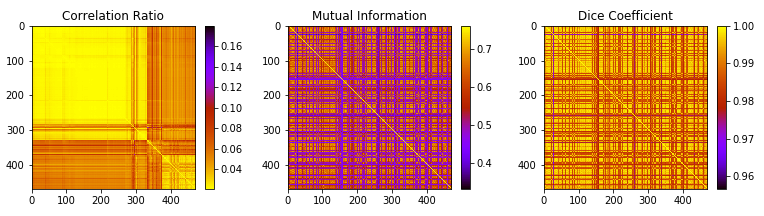
\includegraphics[width=1\textwidth]{6/figures/similarity-mat-sample.png}
\caption{Examples of the three similarity matrices. Lighter colors represent more desirable values.}
\label{fig:sim-mat-sample}
\end{figure}

An example of the three similarity matrices can be seen in Figure \ref{fig:sim-mat-sample}. The element $e_{i,j}$ represents the value of the given metric between the image volumes represented by row $i$ and column $j$. Each metric measures similarity according to slightly different definitions. In this figure, lighter values represent better metric values while darker values indicate lower similarity.

It is important to note the scales for these three metrics vary. The correlation ratio measures the distance between two items. Lower values for the correlation ratio means there is a smaller distance between the given pair of image volumes. The mutual information measures the shared information between two distributions of samples which may or may not be generated from the same underlying distribution. Higher mutual information values mean more shared information and low values mean less shared information. The Dice coefficient measures the overlap of two binary images. High Dice coefficients indicate a large amount of overlap, with a value of 1.0 indicating a perfect overlap.

The correlation ratio matrix in Figure \ref{fig:sim-mat-sample} suggests that the patient remained relatively still for the first 300 volumes of the image, then moved for about 100 volumes, and remained still in a new position for the last 50 frames of the sequence. The colors representing the correlation ratios correspond to very low values, suggesting there is little patient motion overall.

The Dice coefficient matrix has a similar pattern as the mutual information matrix, but leads to a different conclusion. The Dice coefficient was calculated on an Otsu thresholded version of each image volume. As the values of the Dice coefficients are consistently high, the patient likely did not move much. 

The mutual information matrix shows that the shared information throughout the entire image sequence varies. Using the information from the correlation ratio matrix and the Dice coefficient matrix, it is possible that the variations in the mutual information matrix are due to changes in the rs-fMRI signal caused by BOLD signal changes, spin history effects of motion, and susceptibility effects of motion.

\subsection{*Volume Registration: Sequence Duration Motion}

\begin{figure}
\centering
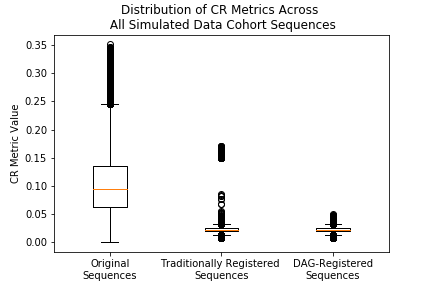
\includegraphics[width=0.5\textwidth]{6/figures/spectr-cr-box.png}
\caption{Boxplots of the values of all correlation ratio matrices for the original sequences, the traditionally registered sequences, and the DAG-registered sequences for the SIMULATED cohort.}
\label{fig:pread-cr-box}
\end{figure}

\begin{table}[]
\centering
\caption{Results of t-tests comparing the descriptive statistics of the correlation ratio matrices for the SIMULATED data.}
\label{tab:pread-cr-ttest}
\begin{tabular}{|c|c|c|c|}
\hline
\textbf{Sequence Type 1 ($S_1$)} &
  \textbf{Original} &
  \textbf{Original} &
  \textbf{\begin{tabular}[c]{@{}c@{}}Traditionally \\ Registered\end{tabular}} \\ \hline
\textbf{Sequence Type 2 ($S_2$)} &
  \textbf{\begin{tabular}[c]{@{}c@{}}Traditionally\\ Registered\end{tabular}} &
  \textbf{\begin{tabular}[c]{@{}c@{}}DAG\\ Registered\end{tabular}} &
  \textbf{\begin{tabular}[c]{@{}c@{}}DAG\\ Registered\end{tabular}} \\ \hline
\begin{tabular}[c]{@{}c@{}}P($S_1$ and $S_2$ \\ have same minimums)\end{tabular} &
  0.3487 &
  0.3407 &
  0.9821 \\ \hline
\begin{tabular}[c]{@{}c@{}}P($S_1$ and $S_2$ \\ have same 1st quartile)\end{tabular} &
  9.750 E -113 &
  1.246 E -112 &
  0.8019 \\ \hline
\begin{tabular}[c]{@{}c@{}}P($S_1$ and $S_2$ \\ have same medians)\end{tabular} &
  5.288 E -88 &
  5.409 E -88 &
  0.9997 \\ \hline
\begin{tabular}[c]{@{}c@{}}P($S_1$ and $S_2$ \\ have same 3rd quartiles)\end{tabular} &
  6.534 E -81 &
  6.730 E -81 &
  0.9577 \\ \hline
\begin{tabular}[c]{@{}c@{}}P($S_1$ and $S_2$ \\ have same maximums)\end{tabular} &
  2.536 E -98 &
  6.180 E -103 &
  0.4068 \\ \hline
\end{tabular}
\end{table}

\begin{figure}
\centering
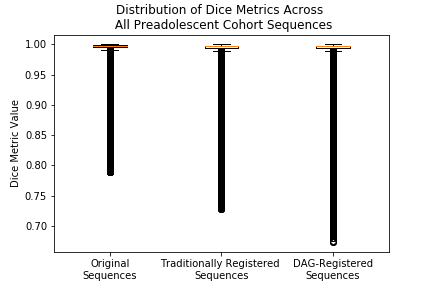
\includegraphics[width=0.5\textwidth]{6/figures/preads-dice-box.png}
\caption{Boxplots of the values of all Dice matrices for the original sequences, the traditionally registered sequences, and the DAG-registered sequences for the preadolescent cohort.}
\label{fig:preads-dice-box}
\end{figure}

\begin{table}[]
\centering
\caption{Results of t-tests comparing the descriptive statistics of the Dice matrices for the preadolescent data.}
\label{tab:preads-dice-ttest}
\begin{tabular}{|c|c|c|c|}
\hline
\textbf{Sequence Type 1 ($S_1$)} &
  \textbf{Original} &
  \textbf{Original} &
  \textbf{\begin{tabular}[c]{@{}c@{}}Traditionally \\ Registered\end{tabular}} \\ \hline
\textbf{Sequence Type 2 ($S_2$)} &
  \textbf{\begin{tabular}[c]{@{}c@{}}Traditionally\\ Registered\end{tabular}} &
  \textbf{\begin{tabular}[c]{@{}c@{}}DAG\\ Registered\end{tabular}} &
  \textbf{\begin{tabular}[c]{@{}c@{}}DAG\\ Registered\end{tabular}} \\ \hline
\begin{tabular}[c]{@{}c@{}}P($S_1$ and $S_2$ \\ have same minimums)\end{tabular} &
  0.770 &
  0.695 &
  0.916 \\ \hline
\begin{tabular}[c]{@{}c@{}}P($S_1$ and $S_2$ \\ have same 1st quartile)\end{tabular} &
  0.976 &
  0.906 &
  0.880 \\ \hline
\begin{tabular}[c]{@{}c@{}}P($S_1$ and $S_2$ \\ have same medians)\end{tabular} &
  0.883 &
  0.562 &
  0.643 \\ \hline
\begin{tabular}[c]{@{}c@{}}P($S_1$ and $S_2$ \\ have same 3rd quartiles)\end{tabular} &
  0.000343 &
  0.000586 &
  0.390 \\ \hline
\begin{tabular}[c]{@{}c@{}}P($S_1$ and $S_2$ \\ have same maximums)\end{tabular} &
  1.0 &
  1.0 &
  1.0 \\ \hline
\end{tabular}
\end{table}

\begin{figure}
\centering
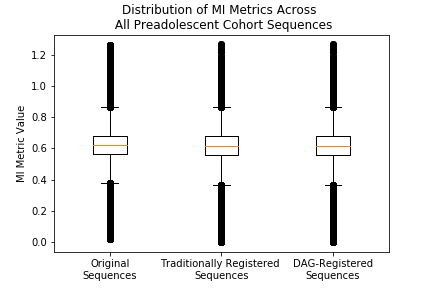
\includegraphics[width=0.5\textwidth]{6/figures/preads-mi-box.png}
\caption{Boxplots of the values of all mutual information matrices for the original sequences, the traditionally registered sequences, and the DAG-registered sequences for the preadolescent cohort.}
\label{fig:preads-mi-box}
\end{figure}

\begin{table}[]
\centering
\caption{Results of t-tests comparing the descriptive statistics of the MI matrices for the preadolescent data.}
\label{tab:preads-mi-ttest}
\begin{tabular}{|c|c|c|c|}
\hline
\textbf{Sequence Type 1 ($S_1$)} &
  \textbf{Original} &
  \textbf{Original} &
  \textbf{\begin{tabular}[c]{@{}c@{}}Traditionally \\ Registered\end{tabular}} \\ \hline
\textbf{Sequence Type 2 ($S_2$)} &
  \textbf{\begin{tabular}[c]{@{}c@{}}Traditionally\\ Registered\end{tabular}} &
  \textbf{\begin{tabular}[c]{@{}c@{}}DAG\\ Registered\end{tabular}} &
  \textbf{\begin{tabular}[c]{@{}c@{}}DAG\\ Registered\end{tabular}} \\ \hline
\begin{tabular}[c]{@{}c@{}}P($S_1$ and $S_2$ \\ have same minimums)\end{tabular} &
  0.624 &
  0.718 &
  0.896 \\ \hline
\begin{tabular}[c]{@{}c@{}}P($S_1$ and $S_2$ \\ have same 1st quartile)\end{tabular} &
  0.489 &
  0.497 &
  0.992 \\ \hline
\begin{tabular}[c]{@{}c@{}}P($S_1$ and $S_2$ \\ have same medians)\end{tabular} &
  0.364 &
  0.324 &
  0.928 \\ \hline
\begin{tabular}[c]{@{}c@{}}P($S_1$ and $S_2$ \\ have same 3rd quartiles)\end{tabular} &
  0.121 &
  0.0882 &
  0.851 \\ \hline
\begin{tabular}[c]{@{}c@{}}P($S_1$ and $S_2$ \\ have same maximums)\end{tabular} &
  0.946 &
  0.932 &
  0.987 \\ \hline
\end{tabular}
\end{table}

The distributions of the metrics matrices were compared to each other using the Kolmogorov-Smirnov test for each sequence type. The metrics for the Dice matrices and the mutual information matrices were determined to be from different distributions for each sequence type at p < 0.005.

%-----------------------------------------------------------------
\section{Neonatal Cohort}

\subsection{Volume Registration: Power Thresholds}

\begin{figure}[t]
	\centering
	\begin{subfigure}{0.4\textwidth}
		\centering
		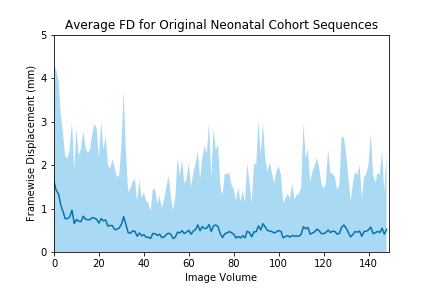
\includegraphics[width=1.0\textwidth]{6/figures/neonates-bold-fd-150.png}
		\caption{FD of Original Sequences.}
	\end{subfigure}
	\hspace{0.05\textwidth}
	\begin{subfigure}{0.4\textwidth}
		\centering
		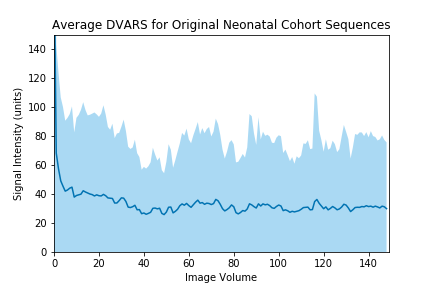
\includegraphics[width=1.0\textwidth]{6/figures/neonates-bold-dvars-150.png}
		\caption{DVARS of Original Sequences.}
	\end{subfigure}
	
	\begin{subfigure}{0.4\textwidth}
		\centering
		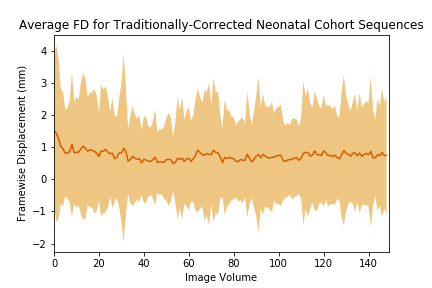
\includegraphics[width=1.0\textwidth]{6/figures/neonates-trad-fd-150.png}
		\caption{FD of Traditionally Registered Sequences.}
	\end{subfigure}
	\hspace{0.05\textwidth}
	\begin{subfigure}{0.4\textwidth}
		\centering
		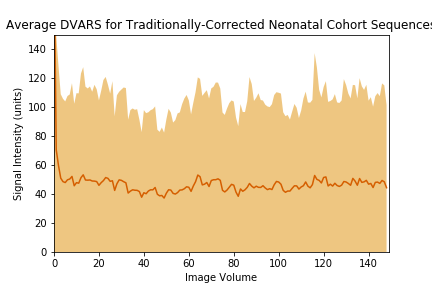
\includegraphics[width=1.0\textwidth]{6/figures/neonates-trad-dvars-150.png}
		\caption{DVARS of Traditionally Registered Sequences.}
	\end{subfigure}
	
	\begin{subfigure}{0.4\textwidth}
		\centering
		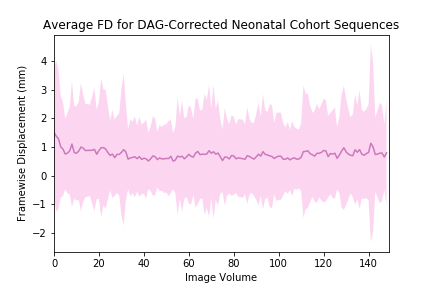
\includegraphics[width=1.0\textwidth]{6/figures/neonates-dag-fd-150.png}
		\caption{FD of DAG-Registered Sequences.}
	\end{subfigure}
	\hspace{0.05\textwidth}
	\begin{subfigure}{0.4\textwidth}
		\centering
		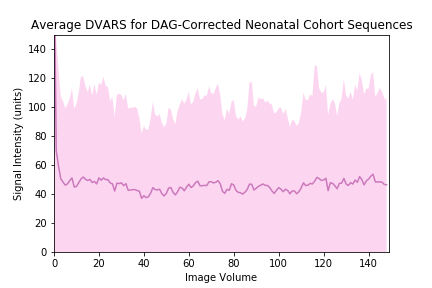
\includegraphics[width=1.0\textwidth]{6/figures/neonates-dag-dvars-150.png}
		\caption{DVARS of DAG-Registered Sequences.}
	\end{subfigure}
\caption{The means and standard deviations of the FD and DVARS metrics for all neonatal images both before and after registration.}
\label{fig:neonate-power-dists}
\end{figure}

\begin{table}[h!]
\centering
\caption{The number and percentage of image volumes across all sequences in the neonatal cohort which meet the usability thresholds of FD \textless 0.2 mm and DVARS \textless 2.5\%.}
\label{tab:neonate-power-thresh}
\begin{tabular}{|c|c|c|c|}
\hline
\textbf{Threshold Met} &
  \textbf{\begin{tabular}[c]{@{}c@{}}Original\\  Sequences\end{tabular}} &
  \textbf{\begin{tabular}[c]{@{}c@{}}Traditionally Registered \\ Sequences\end{tabular}} &
  \textbf{\begin{tabular}[c]{@{}c@{}}DAG-Registered \\ Sequences\end{tabular}} \\ \hline
FD (count)    & 16495  & 14264 & 14173 \\ \hline
DVARS (count) & 16820  & 13903 & 13752 \\ \hline
Both (count)  & 15332  & 12837 & 12684 \\ \hline
FD (\%)       & 69.59  & 60.18 & 59.79 \\ \hline
DVARS(\%)     & 70.96  & 58.65 & 58.02 \\ \hline
Both (\%)     & 64.68  & 54.16 & 53.51 \\ \hline
\end{tabular}
\end{table}

Table \ref{tab:neonate-power-thresh} contains the number and percentages of image volumes from the whole neonatal cohort which meet the FD and DVARS thresholds. The total number of image volumes in across all sequences of a single type was 23704.

\begin{table}[h!]
\centering
\caption{Results from the t-tests comparing the counts for the numbers of images meeting the FD, DVARS, and FD and DVARS thresholds for sequence type $S_1$ and sequence type $S_2$.}
\label{tab:neonate-power-ttest}
\begin{tabular}{|c|c|c|c|}
\hline
\textbf{Sequence Type 1 ($S_1$)} &
  \textbf{Original} &
  \textbf{Original} &
  \textbf{\begin{tabular}[c]{@{}c@{}}Traditionally \\ Registered\end{tabular}} \\ \hline
\textbf{Sequence Type 2 ($S_2$)} &
  \textbf{\begin{tabular}[c]{@{}c@{}}Traditionally\\ Registered\end{tabular}} &
  \textbf{\begin{tabular}[c]{@{}c@{}}DAG\\ Registered\end{tabular}} &
  \textbf{\begin{tabular}[c]{@{}c@{}}DAG\\ Registered\end{tabular}} \\ \hline
\begin{tabular}[c]{@{}c@{}}P($S_1$ and $S_2$ have \\ same FD counts)\end{tabular} &
  0.0110 &
  0.00813 &
  0.924 \\ \hline
\begin{tabular}[c]{@{}c@{}}P($S_1$ and $S_2$ have \\ same DVARS counts)\end{tabular} &
  0.00163 &
  0.000942 &
  0.880 \\ \hline
\begin{tabular}[c]{@{}c@{}}P($S_1$ and $S_2$ have \\ same FD and DVARS counts)\end{tabular} &
  0.00779 &
  0.00475 &
  0.879 \\ \hline
\end{tabular}
\end{table}

Table \ref{tab:neonate-power-ttest} shows the results of a set of t-tests which determine if the distribution of metric X for sequence type $S_1$ is the same as the distribution of metric X for sequence type $S_2$.

\begin{table}[h!]
\centering
\caption{The number of subjects whose sequences of types $S_1$ and $S_2$ had different FD distributions.}
\label{tab:neonate-fd-kstest}
\begin{tabular}{|c|c|c|c|}
\hline
\textbf{\begin{tabular}[c]{@{}c@{}}\# Sequences \\  Type 1 ($S_1$)\end{tabular}} &
  \textbf{\begin{tabular}[c]{@{}c@{}}\# Sequences \\ Type 2 ($S_2$)\end{tabular}} &
  \textbf{\begin{tabular}[c]{@{}c@{}}\# Sequences \\ p \textless 0.05\end{tabular}} &
  \textbf{\begin{tabular}[c]{@{}c@{}}\# Sequences \\ p \textless 0.005\end{tabular}} \\ \hline
Original                                                            & \begin{tabular}[c]{@{}c@{}}Traditionally\\ Registered\end{tabular} & 36	 & 32 \\ \hline
Original                                                            & \begin{tabular}[c]{@{}c@{}}DAG\\ Registered\end{tabular}           & 42 & 38 \\ \hline
\begin{tabular}[c]{@{}c@{}}Traditionally \\ Registered\end{tabular} & \begin{tabular}[c]{@{}c@{}}DAG\\ Registered\end{tabular}           & 13 & 5 \\ \hline
\end{tabular}
\end{table}

\begin{table}[h!]
\centering
\caption{The number of subjects whose sequences of types $S_1$ and $S_2$ had different DVARS distributions.}
\label{tab:neonate-dvars-kstest}
\begin{tabular}{|c|c|c|c|}
\hline
\textbf{\begin{tabular}[c]{@{}c@{}}\# Sequences \\ Type 1($S_1$)\end{tabular}} &
  \textbf{\begin{tabular}[c]{@{}c@{}}\# Sequences \\ Type 2 ($S_2$)\end{tabular}} &
  \textbf{\begin{tabular}[c]{@{}c@{}}\# Sequences \\ p \textless 0.05\end{tabular}} &
  \textbf{\begin{tabular}[c]{@{}c@{}}\# Sequences \\ p \textless 0.005\end{tabular}} \\ \hline
Original                                                            & \begin{tabular}[c]{@{}c@{}}Traditionally\\ Registered\end{tabular} & 44 & 39 \\ \hline
Original                                                            & \begin{tabular}[c]{@{}c@{}}DAG\\ Registered\end{tabular}           & 45 & 44 \\ \hline
\begin{tabular}[c]{@{}c@{}}Traditionally \\ Registered\end{tabular} & \begin{tabular}[c]{@{}c@{}}DAG\\ Registered\end{tabular}           & 11  & 5  \\ \hline
\end{tabular}
\end{table}

\subsection{*Volume Registration: Sequence Duration Motion}

\begin{figure}
\centering
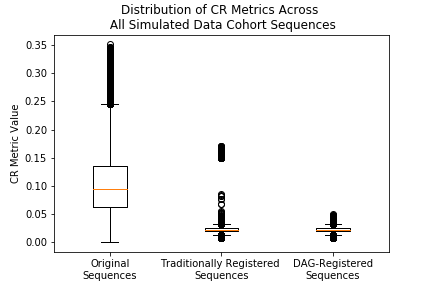
\includegraphics[width=0.5\textwidth]{6/figures/spectr-cr-box.png}
\caption{Boxplots of the values of all correlation ratio matrices for the original sequences, the traditionally registered sequences, and the DAG-registered sequences for the SIMULATED cohort.}
\label{fig:neonates-cr-box}
\end{figure}

\begin{table}[]
\centering
\caption{Results of t-tests comparing the descriptive statistics of the correlation ratio matrices for the SIMULATED data.}
\label{tab:neonates-cr-ttest}
\begin{tabular}{|c|c|c|c|}
\hline
\textbf{Sequence Type 1 ($S_1$)} &
  \textbf{Original} &
  \textbf{Original} &
  \textbf{\begin{tabular}[c]{@{}c@{}}Traditionally \\ Registered\end{tabular}} \\ \hline
\textbf{Sequence Type 2 ($S_2$)} &
  \textbf{\begin{tabular}[c]{@{}c@{}}Traditionally\\ Registered\end{tabular}} &
  \textbf{\begin{tabular}[c]{@{}c@{}}DAG\\ Registered\end{tabular}} &
  \textbf{\begin{tabular}[c]{@{}c@{}}DAG\\ Registered\end{tabular}} \\ \hline
\begin{tabular}[c]{@{}c@{}}P($S_1$ and $S_2$ \\ have same minimums)\end{tabular} &
  0.3487 &
  0.3407 &
  0.9821 \\ \hline
\begin{tabular}[c]{@{}c@{}}P($S_1$ and $S_2$ \\ have same 1st quartile)\end{tabular} &
  9.750 E -113 &
  1.246 E -112 &
  0.8019 \\ \hline
\begin{tabular}[c]{@{}c@{}}P($S_1$ and $S_2$ \\ have same medians)\end{tabular} &
  5.288 E -88 &
  5.409 E -88 &
  0.9997 \\ \hline
\begin{tabular}[c]{@{}c@{}}P($S_1$ and $S_2$ \\ have same 3rd quartiles)\end{tabular} &
  6.534 E -81 &
  6.730 E -81 &
  0.9577 \\ \hline
\begin{tabular}[c]{@{}c@{}}P($S_1$ and $S_2$ \\ have same maximums)\end{tabular} &
  2.536 E -98 &
  6.180 E -103 &
  0.4068 \\ \hline
\end{tabular}
\end{table}

\begin{figure}
\centering
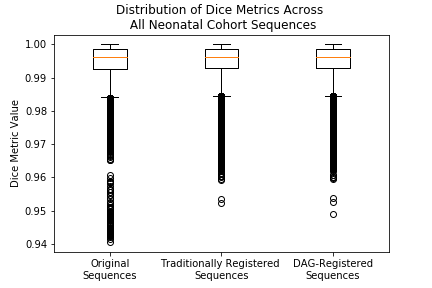
\includegraphics[width=0.5\textwidth]{6/figures/neonates-dice-box.png}
\caption{Boxplots of the values of all Dice matrices for the original sequences, the traditionally registered sequences, and the DAG-registered sequences for the neonatal cohort.}
\label{fig:neonates-dice-box}
\end{figure}

\begin{table}[]
\centering
\caption{Results of t-tests comparing the descriptive statistics of the Dice matrices for the neonatal cohort.}
\label{tab:neonates-dice-ttest}
\begin{tabular}{|c|c|c|c|}
\hline
\textbf{Sequence Type 1 ($S_1$)} &
  \textbf{Original} &
  \textbf{Original} &
  \textbf{\begin{tabular}[c]{@{}c@{}}Traditionally \\ Registered\end{tabular}} \\ \hline
\textbf{Sequence Type 2 ($S_2$)} &
  \textbf{\begin{tabular}[c]{@{}c@{}}Traditionally\\ Registered\end{tabular}} &
  \textbf{\begin{tabular}[c]{@{}c@{}}DAG\\ Registered\end{tabular}} &
  \textbf{\begin{tabular}[c]{@{}c@{}}DAG\\ Registered\end{tabular}} \\ \hline
\begin{tabular}[c]{@{}c@{}}P($S_1$ and $S_2$ \\ have same minimums)\end{tabular} &
  0.523 &
  0.542 &
  0.977 \\ \hline
\begin{tabular}[c]{@{}c@{}}P($S_1$ and $S_2$ \\ have same 1st quartile)\end{tabular} &
  0.468 &
  0.515 &
  0.933 \\ \hline
\begin{tabular}[c]{@{}c@{}}P($S_1$ and $S_2$ \\ have same medians)\end{tabular} &
  0.329 &
  0.292 &
  0.937 \\ \hline
\begin{tabular}[c]{@{}c@{}}P($S_1$ and $S_2$ \\ have same 3rd quartiles)\end{tabular} &
  0.149 &
  0.115 &
  0.890 \\ \hline
\begin{tabular}[c]{@{}c@{}}P($S_1$ and $S_2$ \\ have same maximums)\end{tabular} &
  1.0 &
  1.0 &
  1.0 \\ \hline
\end{tabular}
\end{table}

\begin{figure}
\centering
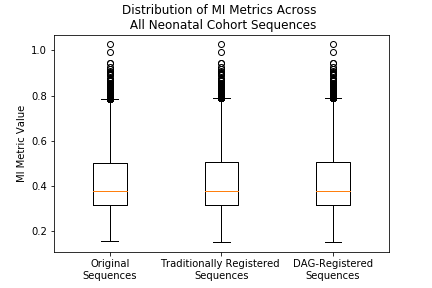
\includegraphics[width=0.5\textwidth]{6/figures/neonates-mi-box.png}
\caption{Boxplots of the values of all mutual information matrices for the original sequences, the traditionally registered sequences, and the DAG-registered sequences for the neonatal cohort.}
\label{fig:neonates-mi-box}
\end{figure}

\begin{table}[]
\centering
\caption{Results of t-tests comparing the descriptive statistics of the MI matrices for the neonatal data.}
\label{tab:neonates-mi-ttest}
\begin{tabular}{|c|c|c|c|}
\hline
\textbf{Sequence Type 1 ($S_1$)} &
  \textbf{Original} &
  \textbf{Original} &
  \textbf{\begin{tabular}[c]{@{}c@{}}Traditionally \\ Registered\end{tabular}} \\ \hline
\textbf{Sequence Type 2 ($S_2$)} &
  \textbf{\begin{tabular}[c]{@{}c@{}}Traditionally\\ Registered\end{tabular}} &
  \textbf{\begin{tabular}[c]{@{}c@{}}DAG\\ Registered\end{tabular}} &
  \textbf{\begin{tabular}[c]{@{}c@{}}DAG\\ Registered\end{tabular}} \\ \hline
\begin{tabular}[c]{@{}c@{}}P($S_1$ and $S_2$ \\ have same minimums)\end{tabular} &
  0.853 &
  0.874 &
  0.978 \\ \hline
\begin{tabular}[c]{@{}c@{}}P($S_1$ and $S_2$ \\ have same 1st quartile)\end{tabular} &
  0.794 &
  0.809 &
  0.985 \\ \hline
\begin{tabular}[c]{@{}c@{}}P($S_1$ and $S_2$ \\ have same medians)\end{tabular} &
  0.762 &
  0.758 &
  0.996 \\ \hline
\begin{tabular}[c]{@{}c@{}}P($S_1$ and $S_2$ \\ have same 3rd quartiles)\end{tabular} &
  0.755 &
  0.743 &
  0.987 \\ \hline
\begin{tabular}[c]{@{}c@{}}P($S_1$ and $S_2$ \\ have same maximums)\end{tabular} &
  0.956 &
  0.938 &
  0.982 \\ \hline
\end{tabular}
\end{table}

The distributions of the metrics matrices were compared to each other using the Kolmogorov-Smirnov test for each sequence type. The metrics for the Dice matrices and the mutual information matrices were determined to be from different distributions for each sequence type at p < 0.005.

\section{*Fetal Cohort}

\subsection{Brain}

\subsubsection{Volume Registration: Power Thresholds}


\begin{figure}[t]
	\centering
	\begin{subfigure}{0.4\textwidth}
		\centering
		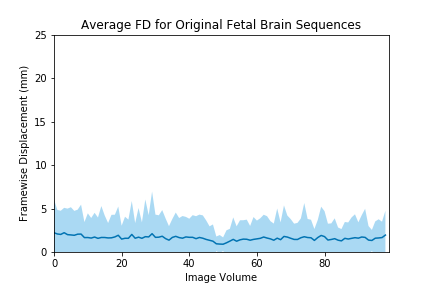
\includegraphics[width=1.0\textwidth]{6/figures/fetal-brain-bold-fd-150.png}
		\caption{FD of Original Sequences.}
	\end{subfigure}
	\hspace{0.05\textwidth}
	\begin{subfigure}{0.4\textwidth}
		\centering
		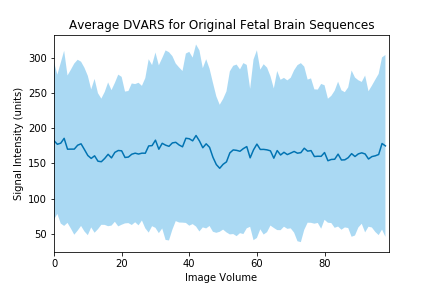
\includegraphics[width=1.0\textwidth]{6/figures/fetal-brain-bold-dvars-150.png}
		\caption{DVARS of Original Sequences.}
	\end{subfigure}
	
	\begin{subfigure}{0.4\textwidth}
		\centering
		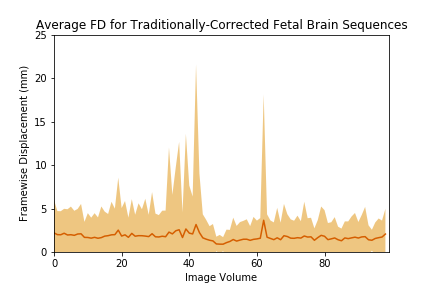
\includegraphics[width=1.0\textwidth]{6/figures/fetal-brain-trad-fd-150.png}
		\caption{FD of Traditionally Registered Sequences.}
	\end{subfigure}
	\hspace{0.05\textwidth}
	\begin{subfigure}{0.4\textwidth}
		\centering
		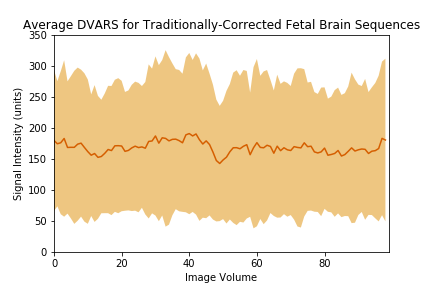
\includegraphics[width=1.0\textwidth]{6/figures/fetal-brain-trad-dvars-150.png}
		\caption{DVARS of Traditionally Registered Sequences.}
	\end{subfigure}
	
	\begin{subfigure}{0.4\textwidth}
		\centering
		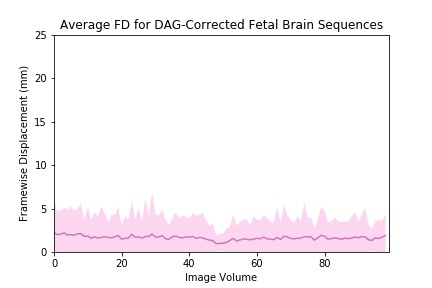
\includegraphics[width=1.0\textwidth]{6/figures/fetal-brain-dag-fd-150.png}
		\caption{FD of DAG-Registered Sequences.}
	\end{subfigure}
	\hspace{0.05\textwidth}
	\begin{subfigure}{0.4\textwidth}
		\centering
		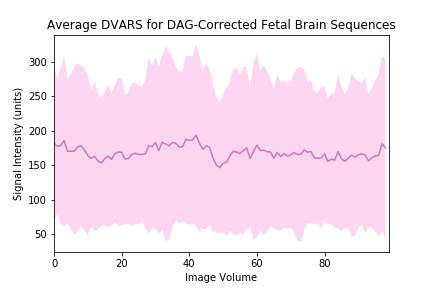
\includegraphics[width=1.0\textwidth]{6/figures/fetal-brain-dag-dvars-150.png}
		\caption{DVARS of DAG-Registered Sequences.}
	\end{subfigure}
\caption{The means and standard deviations of the FD and DVARS metrics for all fetal brain images both before and after registration.}
\label{fig:fetal-brain-power-dists}
\end{figure}

\begin{table}[h!]
\centering
\caption{The number and percentage of image volumes across all sequences in the fetal brain image data set which meet the usability thresholds of FD \textless 0.2 mm and DVARS \textless 2.5\%.}
\label{tab:fetal-brain-power-thresh}
\begin{tabular}{|c|c|c|c|}
\hline
\textbf{Threshold Met} &
  \textbf{\begin{tabular}[c]{@{}c@{}}Original\\  Sequences\end{tabular}} &
  \textbf{\begin{tabular}[c]{@{}c@{}}Traditionally Registered \\ Sequences\end{tabular}} &
  \textbf{\begin{tabular}[c]{@{}c@{}}DAG-Registered \\ Sequences\end{tabular}} \\ \hline
FD (count)    & 575    & 539   & 561 \\ \hline
DVARS (count) & 7      & 84    & 7 \\ \hline
Both (count)  & 7      & 80    & 7 \\ \hline
FD (\%)       & 4.775  & 4.503 & 4.659 \\ \hline
DVARS(\%)     & 0.058  & 0.702 & 0.058 \\ \hline
Both (\%)     & 0.058  & 0.668 & 0.058 \\ \hline
\end{tabular}
\end{table}

Table \ref{tab:fetal-brain-power-thresh} contains the number and percentages of image volumes from the whole neonatal cohort which meet the FD and DVARS thresholds. The total number of image volumes in across all sequences of a single type was 12041.

\begin{table}[h!]
\centering
\caption{Results from the t-tests comparing the counts for the numbers of images meeting the FD, DVARS, and FD and DVARS thresholds for fetal brain sequence type $S_1$ and sequence type $S_2$.}
\label{tab:fetal-brain-power-ttest}
\begin{tabular}{|c|c|c|c|}
\hline
\textbf{Sequence Type 1 ($S_1$)} &
  \textbf{Original} &
  \textbf{Original} &
  \textbf{\begin{tabular}[c]{@{}c@{}}Traditionally \\ Registered\end{tabular}} \\ \hline
\textbf{Sequence Type 2 ($S_2$)} &
  \textbf{\begin{tabular}[c]{@{}c@{}}Traditionally\\ Registered\end{tabular}} &
  \textbf{\begin{tabular}[c]{@{}c@{}}DAG\\ Registered\end{tabular}} &
  \textbf{\begin{tabular}[c]{@{}c@{}}DAG\\ Registered\end{tabular}} \\ \hline
\begin{tabular}[c]{@{}c@{}}P($S_1$ and $S_2$ have \\ same FD counts)\end{tabular} &
  0.811 &
  0.926 &
  0.883 \\ \hline
\begin{tabular}[c]{@{}c@{}}P($S_1$ and $S_2$ have \\ same DVARS counts)\end{tabular} &
  0.159 &
  1.0 &
  0.159 \\ \hline
\begin{tabular}[c]{@{}c@{}}P($S_1$ and $S_2$ have \\ same FD and DVARS counts)\end{tabular} &
  0.159 &
  1.0 &
  0.159 \\ \hline
\end{tabular}
\end{table}

Table \ref{tab:fetal-brain-power-ttest} shows the results of a set of t-tests which determine if the distribution of metric X for sequence type $S_1$ is the same as the distribution of metric X for sequence type $S_2$. Fetal brain.

\begin{table}[h!]
\centering
\caption{The number of subjects whose sequences of types $S_1$ and $S_2$ had different FD distributions according to the Kolmogorov-Smirnov test.}
\label{tab:fetal-brain-fd-kstest}
\begin{tabular}{|c|c|c|c|}
\hline
\textbf{\begin{tabular}[c]{@{}c@{}}\# Sequences \\ Type 1 ($S_1$)\end{tabular}} &
  \textbf{\begin{tabular}[c]{@{}c@{}}\# Sequences \\ Type 2 ($S_2$)\end{tabular}} &
  \textbf{\begin{tabular}[c]{@{}c@{}}\# Sequences \\ p \textless 0.05\end{tabular}} &
  \textbf{\begin{tabular}[c]{@{}c@{}}\# Sequences \\ p \textless 0.005\end{tabular}} \\ \hline
Original                                                            & \begin{tabular}[c]{@{}c@{}}Traditionally\\ Registered\end{tabular} & 14 & 9 \\ \hline
Original                                                            & \begin{tabular}[c]{@{}c@{}}DAG\\ Registered\end{tabular}           & 2  & 2 \\ \hline
\begin{tabular}[c]{@{}c@{}}Traditionally \\ Registered\end{tabular} & \begin{tabular}[c]{@{}c@{}}DAG\\ Registered\end{tabular}           & 13 & 9 \\ \hline
\end{tabular}
\end{table}

\begin{table}[h!]
\centering
\caption{The number of subjects whose sequences of types $S_1$ and $S_2$ had different DVARS distributions according to the Kolmogorov-Smirnov test.}
\label{tab:fetal-brain-dvars-kstest}
\begin{tabular}{|c|c|c|c|}
\hline
\textbf{\begin{tabular}[c]{@{}c@{}}\# Sequences \\ Type 1 ($S_1$)\end{tabular}} &
  \textbf{\begin{tabular}[c]{@{}c@{}}\# Sequences \\ Type 2 ($S_2$)\end{tabular}} &
  \textbf{\begin{tabular}[c]{@{}c@{}}\# Sequences \\ p \textless 0.05\end{tabular}} &
  \textbf{\begin{tabular}[c]{@{}c@{}}\# Sequences \\ p \textless 0.005\end{tabular}} \\ \hline
Original                                                            & \begin{tabular}[c]{@{}c@{}}Traditionally\\ Registered\end{tabular} & 3 & 3 \\ \hline
Original                                                            & \begin{tabular}[c]{@{}c@{}}DAG\\ Registered\end{tabular}           & 2 & 1 \\ \hline
\begin{tabular}[c]{@{}c@{}}Traditionally \\ Registered\end{tabular} & \begin{tabular}[c]{@{}c@{}}DAG\\ Registered\end{tabular}           & 2  & 2  \\ \hline
\end{tabular}
\end{table}

\begin{table}[h!]
\centering
\caption{Comparing the FD and DVARS distributions for all image volumes for sequence types $S_1$ and $S_2$ for the fetal brain images.}
\label{tab:fetal-brain-ks-all}
\begin{tabular}{|c|c|c|c|}
\hline
\textbf{Sequence Type 1} & \textbf{Sequence Type 2}                                           & \textbf{FD p-value} & \textbf{DVARS p-value} \\ \hline
Original                 & \begin{tabular}[c]{@{}c@{}}Traditionally\\ Registered\end{tabular} & 2.712 E -10         & 8.019 E -6             \\ \hline
Original                 & \begin{tabular}[c]{@{}c@{}}DAG\\ Registered\end{tabular}           & 0.703               & 0.934                  \\ \hline
\begin{tabular}[c]{@{}c@{}}Traditionally \\ Registered\end{tabular} & \begin{tabular}[c]{@{}c@{}}DAG\\ Registered\end{tabular} & 4.88 E -8 & 0.000380 \\ \hline
\end{tabular}
\end{table}

\subsubsection{Volume Registration: Sequence Duration Motion}

\subsection{Placenta}

\subsubsection{Volume Registration: Power Thresholds}


\begin{table}[h!]
\centering
\caption{The number and percentage of image volumes across all sequences in the fetal placenta image data set which meet the usability thresholds of FD \textless 0.2 mm and DVARS \textless 2.5\%.}
\label{tab:fetal-placenta-power-thresh}
\begin{tabular}{|c|c|c|c|}
\hline
\textbf{Threshold Met} &
  \textbf{\begin{tabular}[c]{@{}c@{}}Original\\  Sequences\end{tabular}} &
  \textbf{\begin{tabular}[c]{@{}c@{}}Traditionally Registered \\ Sequences\end{tabular}} &
  \textbf{\begin{tabular}[c]{@{}c@{}}DAG-Registered \\ Sequences\end{tabular}} \\ \hline
FD (count)    & 575    & 539   & 561 \\ \hline
DVARS (count) & 7      & 84    & 7 \\ \hline
Both (count)  & 7      & 80    & 7 \\ \hline
FD (\%)       & 4.775  & 4.503 & 4.659 \\ \hline
DVARS(\%)     & 0.058  & 0.702 & 0.058 \\ \hline
Both (\%)     & 0.058  & 0.668 & 0.058 \\ \hline
\end{tabular}
\end{table}

Table \ref{tab:fetal-brain-power-thresh} contains the number and percentages of image volumes from the whole neonatal cohort which meet the FD and DVARS thresholds. The total number of image volumes in across all sequences of a single type was 12041.

\begin{table}[h!]
\centering
\caption{Results from the t-tests comparing the counts for the numbers of images meeting the FD, DVARS, and FD and DVARS thresholds for fetal brain sequence type $S_1$ and sequence type $S_2$.}
\label{tab:fetal-brain-power-ttest}
\begin{tabular}{|c|c|c|c|}
\hline
\textbf{Sequence Type 1 ($S_1$)} &
  \textbf{Original} &
  \textbf{Original} &
  \textbf{\begin{tabular}[c]{@{}c@{}}Traditionally \\ Registered\end{tabular}} \\ \hline
\textbf{Sequence Type 2 ($S_2$)} &
  \textbf{\begin{tabular}[c]{@{}c@{}}Traditionally\\ Registered\end{tabular}} &
  \textbf{\begin{tabular}[c]{@{}c@{}}DAG\\ Registered\end{tabular}} &
  \textbf{\begin{tabular}[c]{@{}c@{}}DAG\\ Registered\end{tabular}} \\ \hline
\begin{tabular}[c]{@{}c@{}}P($S_1$ and $S_2$ have \\ same FD counts)\end{tabular} &
  0.811 &
  0.926 &
  0.883 \\ \hline
\begin{tabular}[c]{@{}c@{}}P($S_1$ and $S_2$ have \\ same DVARS counts)\end{tabular} &
  0.159 &
  1.0 &
  0.159 \\ \hline
\begin{tabular}[c]{@{}c@{}}P($S_1$ and $S_2$ have \\ same FD and DVARS counts)\end{tabular} &
  0.159 &
  1.0 &
  0.159 \\ \hline
\end{tabular}
\end{table}

Table \ref{tab:fetal-brain-power-ttest} shows the results of a set of t-tests which determine if the distribution of metric X for sequence type $S_1$ is the same as the distribution of metric X for sequence type $S_2$. Fetal brain.

\begin{table}[h!]
\centering
\caption{The number of subjects whose sequences of types $S_1$ and $S_2$ had different FD distributions according to the Kolmogorov-Smirnov test.}
\label{tab:fetal-brain-fd-kstest}
\begin{tabular}{|c|c|c|c|}
\hline
\textbf{\begin{tabular}[c]{@{}c@{}}\# Sequences \\ Type 1 ($S_1$)\end{tabular}} &
  \textbf{\begin{tabular}[c]{@{}c@{}}\# Sequences \\ Type 2 ($S_2$)\end{tabular}} &
  \textbf{\begin{tabular}[c]{@{}c@{}}\# Sequences \\ p \textless 0.05\end{tabular}} &
  \textbf{\begin{tabular}[c]{@{}c@{}}\# Sequences \\ p \textless 0.005\end{tabular}} \\ \hline
Original                                                            & \begin{tabular}[c]{@{}c@{}}Traditionally\\ Registered\end{tabular} & 14 & 9 \\ \hline
Original                                                            & \begin{tabular}[c]{@{}c@{}}DAG\\ Registered\end{tabular}           & 2  & 2 \\ \hline
\begin{tabular}[c]{@{}c@{}}Traditionally \\ Registered\end{tabular} & \begin{tabular}[c]{@{}c@{}}DAG\\ Registered\end{tabular}           & 13 & 9 \\ \hline
\end{tabular}
\end{table}

\begin{table}[h!]
\centering
\caption{The number of subjects whose sequences of types $S_1$ and $S_2$ had different DVARS distributions according to the Kolmogorov-Smirnov test.}
\label{tab:fetal-brain-dvars-kstest}
\begin{tabular}{|c|c|c|c|}
\hline
\textbf{\begin{tabular}[c]{@{}c@{}}\# Sequences \\ Type 1 ($S_1$)\end{tabular}} &
  \textbf{\begin{tabular}[c]{@{}c@{}}\# Sequences \\ Type 2 ($S_2$)\end{tabular}} &
  \textbf{\begin{tabular}[c]{@{}c@{}}\# Sequences \\ p \textless 0.05\end{tabular}} &
  \textbf{\begin{tabular}[c]{@{}c@{}}\# Sequences \\ p \textless 0.005\end{tabular}} \\ \hline
Original                                                            & \begin{tabular}[c]{@{}c@{}}Traditionally\\ Registered\end{tabular} & 3 & 3 \\ \hline
Original                                                            & \begin{tabular}[c]{@{}c@{}}DAG\\ Registered\end{tabular}           & 2 & 1 \\ \hline
\begin{tabular}[c]{@{}c@{}}Traditionally \\ Registered\end{tabular} & \begin{tabular}[c]{@{}c@{}}DAG\\ Registered\end{tabular}           & 2  & 2  \\ \hline
\end{tabular}
\end{table}

\begin{table}[h!]
\centering
\caption{Comparing the FD and DVARS distributions for all image volumes for sequence types $S_1$ and $S_2$ for the fetal brain images.}
\label{tab:fetal-brain-ks-all}
\begin{tabular}{|c|c|c|c|}
\hline
\textbf{Sequence Type 1} & \textbf{Sequence Type 2}                                           & \textbf{FD p-value} & \textbf{DVARS p-value} \\ \hline
Original                 & \begin{tabular}[c]{@{}c@{}}Traditionally\\ Registered\end{tabular} & 2.712 E -10         & 8.019 E -6             \\ \hline
Original                 & \begin{tabular}[c]{@{}c@{}}DAG\\ Registered\end{tabular}           & 0.703               & 0.934                  \\ \hline
\begin{tabular}[c]{@{}c@{}}Traditionally \\ Registered\end{tabular} & \begin{tabular}[c]{@{}c@{}}DAG\\ Registered\end{tabular} & 4.88 E -8 & 0.000380 \\ \hline
\end{tabular}
\end{table}

\subsubsection{Volume Registration: Sequence Duration Motion}

\section{Motion Patterns}

\subsection{Age Groups}

\subsection{CHD and Control}

\subsection{Preadolescents: Comparing Sites}

\chapter{DISCUSSION}
\label{ch:discussion}

\section{Volume Registration}

The comparison of the simulated and clinical brain rs-fMRIs using the FD and DVARS metrics showed little difference with respect to reducing the positional and signal effects of motion between pairs of subsequent time points. In the set of placenta images, both registration types improved the number of image volumes meeting the DVARS thresholds. These metrics were not considered sufficient for examining the effects of registration on patient motion, so the similarity matrices were employed. For the simulated data cohort, the minimum values and quartiles of the distributions of the Dice and MI matrices increased more for the DAG-registered sequences than for the original sequences. The changes in the similarity matrix distributions was comparable overall for the clinical images.

An additional analysis was performed for the simulated images. The goal of this analysis was to evaluate the effects of volume registration on the brain signal present in an rs-fMRI image. It was found that the DAG-registered sequences had correct voxel classifications when compared to the DMN ROI than the traditional registration did. 

This finding has interesting potential. Subject motion during rs-MRI scans affects both the recorded position and orientation of the subject as well as the established magnetic spin gradients within the skull and the susecptibility recorded in each voxel. The primary focus of volume registration has been to reduce the positional effects of motion. Correction of the spin history effects and the susceptibility effects are considered to be a separate albeit related area of research. The results of the independent component analysis of the simulated images suggest that the DAG-based registration may contribute to the reduction of the signal-based effects of motion. It could potentially be coupled with prospective motion monitoring techniques, $B_0$ field maps, and navigator sequences to address the other half of the motion problem.

All images used in these analyses consisted of brain tissue against an empty background. The images had undergone processing to remove tissues outside the skull either using automated tools or manual segmentation. The use of manual segmentation with multiple annotators has the potential to confound the results of motion correction experiments. The segmentation process may not remove all non-brain tissue from the image. Those images would then contain brain tissue, non-brain tissue, and dark background. The registration process optimizes the alignment of values in a pair of images. In some cases, the registration reach a state where the lowest cost alignment aligns tissue in general and not specifically brain tissue. While these alignments would have the lowest cost, the would not be physically correct. This problem would be difficult to detect in the metrics extracted from the image sequence: the metrics only measure the properties of the voxel values in the sequence, not of the physiological information it contains. 

Specifically, this limitation pertains to our fetal scans. The masks generated during the segmentation process were created to be uniform across the whole sequence. However, fetal motion is highly variable. The subject may drastically change position in the middle of the scan, possibly several times. The manually created masks were developed using a software tool which allows 3D image masks to be applied to an entire 4D image sequence. The masks were required to be created to ensure the fetal brain or placenta would be inside the masked area at all times and therefore may not have removed all tissues that were not of interest.

This limitation can be resolved by incorporating computer vision principles into the anatomical aspects of image segmentation. Filters used in computer vision applications to identify edges, smooth areas, and track objects have great potential when applied to segmenting fetal brain tissue in the presence of motion.

\section{Characterizing Motion}

In addition to the evaluation of motion within the images, clustering techniques were used to identify groups of subjects with similar motion patterns in their original sequences. Agglomerative clustering was used to confirm the existence of similar motion patterns between patients. The agglomerative clustering results consisting of a heatmap and a dendrogram were combined with two sets of labels: the disease status and age group of each subject. Examination of the dendrograms and heatmaps coupled with the labels suggested that subjects in the same age group were more likely to exhibit similar motion patterns to each other than to subjects in other age groups. To reinforce this theory, k-means clustering and spectral clustering were also performed on the data. The labels produced by the clustering techniques were compared to the age group labels. The composition of the clusters reinforces the theory that patient motion patterns vary more between age groups than among age groups.

Additional analyses could be performed to further evaluate the computer detectable differences in patient groups. The models presented in the previous chapter were generated each using a single metric type. Each metric only measures one property of the image volumes. It is possible that combinations of metrics measuring different properties could be used to better separate patient groups. For example, the combination of the FD values and the DVARS values could more comprehensively categorize subjects based on the effects of motion, BOLD signal change, and background noise.

\section{Relation to Existing Work}

\subsection{MRI Simulations} 

The idea of simulated MRIs originated in the 1980s. Bobman et al. suggested a process of MR image synthesis, then demonstrated its validity by creating synthetic spin-echo brain MRIs and comparing the simulated images to clinical images \cite{Bobman1985}. Since then, a number of MRI simulation softwares have been developed. Herein, we discuss two of these tools and compare them to our simulation tool.

The FMRIB group developed a simulation tool called \href{https://fsl.fmrib.ox.ac.uk/fsl/fslwiki/POSSUM}{POSSUM} (Physics-Oriented Simulated Scanner for Understanding MRI) \cite{Drobnjak2006} \cite{Drobnjak2010}. POSSUM offers realistic, physics-based simulation of structural, functional, and diffusion tensor images. It requires a gradient echo pulse sequence and a segmented object with known tissue properties as inputs for the simulation. It allows the user a high degree of control over the physical properties to be simulated. The user has the ability to specify the pulse sequence information, the method for generating brain signal, the addition of motion and noise, and the method for image reconstruction. Both a GUI and a command line interface are available for POSSUM. 

\begin{figure}
\centering
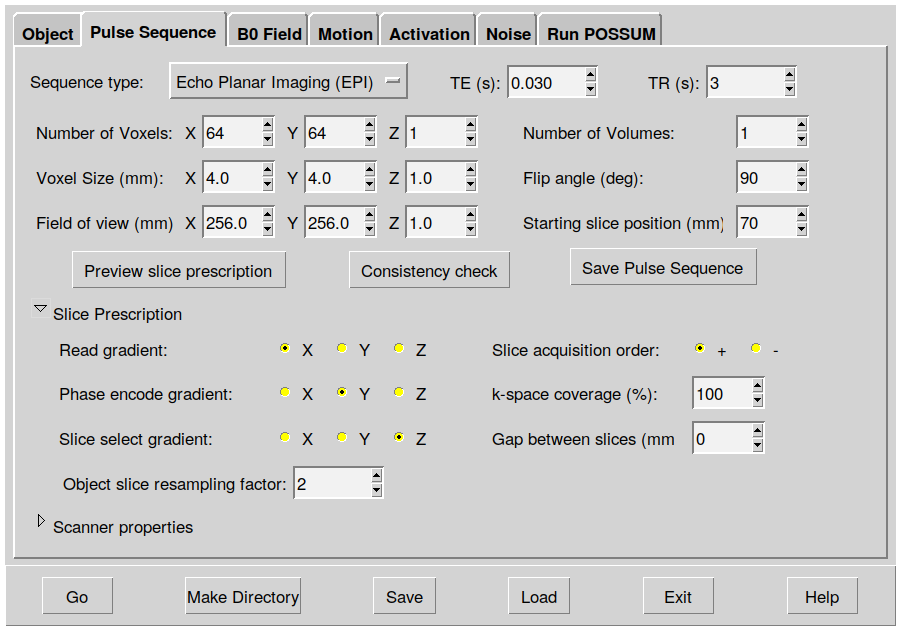
\includegraphics[width=.6\textwidth]{7/possum-gui.png}
\caption{The ``Pulse Sequence'' specifications page in the POSSUM GUI}
\label{fig:possum}
\end{figure}

The biggest drawback to POSSUM is the degree of MR physics knowledge needed to use it effectively. For MR physicists, specifying the details of a pulse sequence may be trivial. For researchers from other fields, customizing pulse sequence parameters, an example of which can be seen in Figure \ref{fig:possum}, can be a challenging task. These customizations may even be unnecessary depending on the goals a researcher hopes to achieve using the simulated data.

If a researcher's goal is to test the impact of a new MRI processing technique on known signals in an image, the BrainWeb MRI simulator might be a better option than POSSUM. BrainWeb was created and is actively developed by the \href{mcgill.ca/bic/}{McConnell Brain Imaging Centre} at McGill University to assist in validation computer-aided MRI analysis tools \cite{kwan1999mri} \cite{collins1998design} \cite{cocosco1997brainweb} \cite{kwan1996extensible}. A set of simulated images have been generated using BrainWeb and are can be found in the BrainWeb Simulated Brain Database (SBD). The SBD contains simulated images for healthy subjects and for subjects who have lesions due to multiple sclerosis.

Custom simulations can be generated on the BrainWeb server by submitting a request via a browser. The simulation request form has three areas which can be customized: the type of brain to simulate, the MR pulse sequence, and the imaging artifacts. The simulation is run on the server and the user is notified via email when the simulated images are ready to download. 

BrainWeb's simulator is slightly more approachable than POSSUM: a limited number of pulse sequence parameters are available to customize and a description is listed next to each parameter in the pulse sequence and imaging artifacts sections. However, the user has slightly less control over the simulated image. The brain models used by BrainWeb are healthy brains or brains with MS lesions. It is not an option for the user to upload an image to use as the structural information in the sequence. For our purposes, the biggest limitation of BrainWeb is that it only simulates structural images. 

Our simulation tool, SPECTr, is one of the few tools which simulates resting-state fMRIs. It offers the opportunity for researchers to explore the effects of their motion correction techniques on BOLD signal, background noise, and patient motion using a lightweight simulation that can be run on a personal computer. It should be noted that SPECTr is not a substitute for the physics-based models in POSSUM and BrainWeb: it is intended to evaluate signal changes in rs-fMRI sequences as a result of post-acquisition image processing.

\subsection{Volume Registration} 

To the best of our knowledge, the only other study that has used a variant of the DAG-based method was performed by Liao et al \cite{Liao2016}. Liao et al’s dataset consisted of 10 fetal rs-fMRIs. In each of these sequences, the fetal brain, fetal liver, and placenta were manually segmented in the first volume of the sequence as well as in five other randomly chosen volumes. These overlap of these manual segmentations before and after registration as measured using the Dice coefficient was used to quantify the amount of motion in each sequence. Even though the Dice coefficients increase more in each sequence after Liao et al.’s registration than after traditional registration, their measure of positional change fails to quantify any changes in position between any other pairs of volumes that do not have manual segmentations. 

The fetal images used in Liao et al.'s study included images of singleton, twin, and triplet pregnancies. There is significant potential value in the study of fetal motion in multifetal pregnancies. Considering the motion patterns alone, it would be expected that the singleton pregnancies have different motion patterns than the multifetal pregnancies

\subsection{Age Group Specific Motion}

It has been established that motion is often correlated with patient age in adolescent population. Satterthwaite et al. specifically designed an imaging study of adolescents ages 8-23 such that patient age and motion were uncorrelated \cite{Satterthwaite2012} % ELEPHANTS check citation
In our study, patient age was described only as fetal, neonatal, or preadolescent despite a range of ages in each group. We establish that there are characteristics of patient motion specific to each group, but we did not consider more granular ranges of patient age. Additional analyses would need to be considered to determine whether post-conceptual age for fetal and neonatal subjects impacts motion characteristics. 

In the fetal cohort, it is possible that there are motion characteristics linked to post-conceptual age. As a fetus grows, the amount of room in the uterus in which it can move decreases. However, as the fetal brain develops, the fetus may begin to move in different ways to test its biological systems. 

Studies involving neonatal cohorts often track two ages for the subjects: the post-conceptual age and the age since birth. The relationship between these two ages and a neonate's brain development could impact the amount of motion exhibited during a scan.
\chapter{Conclusions}
\label{ch:fin}

The two primary goals of this work were to compare two volume registration techniques and to characterize motion in different clinical groups. Five sets of images were used for these experiments: a simulated data set, brain images from three clinical cohorts, and a set of placenta images. 

An rs-fMRI simulation tool was developed to generate data with a known BOLD signal, background signal noise, and patient motion. The base for the structural information in the simulated sequences was the proton density image from the MNI average brain data, while the regions of interest used to generate the simulated BOLD signal were taken from the 90 functional ROI atlases created by Shirer et al. \cite{Shirer2012}. 

The clinical images were obtained as part of prospective, long-term studies of CHD and brain development. The neonatal subjects were recruited from a single site while the fetal subjects were recruited at one of two sites, and the preadolescent subjects were recruited at one of 12 sites in the United States. The sequences differed in length depending on the age group and scanning site. In addition to the images, basic demographic information was gathered for each subject.

All rs-fMRIs from the simulated and clinical data sets underwent both the traditional registration and the DAG-based registration. The original sequences and both types of registered sequences were compared. Four metrics were used for these comparisons. The FD and DVARS metrics were calculated between every image volume $i$ and $i+1$ in each sequence. The Dice and MI similarities were calculated for every possible pair of image volumes $i$ and $j$ in a single sequence. 

The FD and DVARS metrics were compared to the usability thresholds set forth by Power et al. \cite{Power2012}. These thresholds state that an rs-fMRI has sufficiently low quantities of motion if more than 50\% of the volumes in the sequence have FD $<$ 0.2 mm and DVARS $<$ 2.5\% signal intensity units. The number of image volumes meeting these thresholds for each sequence type (original, traditionally registered, and DAG-registered) were calculated and compared using two-sample t-tests. 

Comparing the FD and DVARS metrics for the simulated, preadolescent, neonatal, and fetal brain images to the usability threshold showed that the two registration types had comparable effects with respect to recovering image volumes to the usability standards. Between these four data sets, there were slightly different impacts of each registration type on each cohort, but the registration techniques did not recover statistically significantly different numbers of image volumes. The placenta images, however, demonstrated a statistically significant increase in the number of image volumes meeting the DVARS threshold and the pair of thresholds after registration.

The rs-fMRIs were also compared using matrices of similarity metrics where the value at every row $i$ and column $j$ was the similarity between volumes $i$ and $j$ in the same image sequence. The purpose of these matrices was to better characterize the positional and signal changes due to motion throughout the image sequence. Analysis of the sequence duration motion in the simulated data set showed mixed results. For the simulated sequences, the DAG-based registration was better at improving the range and quartile values of the distribution of the original similarity metrics than the traditional registration was.

One additional analysis on the simulated images was used to compare the traditional and DAG-based registration techniques. The registered images underwent independent component analysis. The components for each image were compared to the DMN ROI to identify the component which correlated best with the simulated BOLD signal. The best matching components were compared voxelwise to the DMN ROI to determine the number of true positive, false positive, true negative, and false negative identifications of component voxels as belonging to the DMN ROI. The DAG-based registration had a higher true positive rate and a lower false positive rate (0.623 and 0.00996) than the traditional registration did (0.587 and 0.104).

After analyzing the volume registration techniques, the patterns of motion in the clinical brain images were characterized into two categories of interest. No detectable groups were identified when the metrics for the original image sequences were clustered and labeled according to disease status. However, analysis of the clusters labeled according to age group suggests that there are detectable differences in the patterns of motion between subjects from different age groups.


%
\appendix
\chapter{Volume Registration Parameters}
\label{appendix:registration-params}

The parameters used for the registration of pairs of image volumes can be seen below.

\begin{lstlisting}
##
# Register a pair of image volumes
#
# Effects: save a copy of the registered image and the 
# registration parameters
#
# @param fixedImgFn The filename of the fixed image 
#                   as a string
# @param movinImgFn The filename of the moving image
#                   as a string
# @param regImgOutFn The filename as a string specifying
#                   where to save the registered moving image
# @param transformPrefix The filename as a string specifying
#                   where to save the transformation matrix   
# @param initialize Optional parameter to specify the location 
#                   of the transform matrix from the
#                   previous registration
# @param regType Optional parameter to specify the type of
#                   registration to use (affine ['Affine'] 
#                   or nonlinear ['Syn']) Default: nonlinear
def registerVolumes(fixedImgFn, movinImgFn, regImgOutFn,
transformPrefix, initialize=None, regtype='nonlinear'):
  # Registration set up: for both Affine and SyN transforms
  reg = Registration()
  reg.inputs.fixed_image = fixedImgFn
  reg.inputs.moving_image = movinImgFn
  reg.inputs.output_transform_prefix = transformPrefix 
  reg.inputs.interpolation = 'NearestNeighbor'
  reg.inputs.dimension = 3
  reg.inputs.write_composite_transform = False 
  reg.inputs.collapse_output_transforms = False
  reg.inputs.initialize_transforms_per_stage = False
  reg.inputs.num_threads = 100
  reg.inputs.output_warped_image = regImgOutFn

  # Registration set up: Specify certain parameters
  # for the Affine registration step
  reg.inputs.transforms = ['Affine']
  reg.inputs.transform_parameters = [(2.0,)]
  reg.inputs.number_of_iterations = [[1500, 200]] 
  reg.inputs.metric = ['CC'] 
  reg.inputs.metric_weight = [1]
  reg.inputs.radius_or_number_of_bins = [5] 
  reg.inputs.convergence_threshold = [1.e-8]
  reg.inputs.convergence_window_size = [20]
  reg.inputs.smoothing_sigmas = [[1,0]]
  reg.inputs.sigma_units = ['vox']
  reg.inputs.shrink_factors = [[2,1]]
  reg.inputs.use_estimate_learning_rate_once = [True]
  reg.inputs.use_histogram_matching = [True] # Default

  # Registration set up: nonlinear transforms only
  if regtype == 'nonlinear':
    reg.inputs.transforms.append('SyN')
    reg.inputs.transform_parameters.append((0.25, 3.0, 0.0))
    reg.inputs.number_of_iterations.append([100, 50, 30])
    reg.inputs.metric.append('CC')
    reg.inputs.metric_weight.append(1)
    reg.inputs.radius_or_number_of_bins.append(5)
    reg.inputs.convergence_threshold.append(1.e-9)
    reg.inputs.convergence_window_size.append(20)
    reg.inputs.smoothing_sigmas.append([2,1,0])
    reg.inputs.sigma_units.append('vox')
    reg.inputs.shrink_factors.append([3,2,1])
    reg.inputs.use_estimate_learning_rate_once.append(True)
    reg.inputs.use_histogram_matching.append(True) # Default

  # If the registration is initialized, add parameters
  if initialize is not None:
    reg.inputs.initial_moving_transform = initialize
    reg.inputs.invert_initial_moving_transform = False

  # Keep the user updated with the status of the registration
  print("Starting", regtype, "registration for", regImgOutFn)
    
  # Run the registration
  reg.run()
    
  # Keep the user updated with the status of the registration
  print("Finished", regtype, "registration for", regImgOutFn)

\end{lstlisting}
\chapter{Supplemental Statistical Tables}
\label{appendix:results}

\section{Simulated Data}

%\vspace{-10mm}
\begin{table}[!ht]
\centering
\caption{Results from the t-tests comparing the counts for the numbers of images meeting the FD, DVARS, and FD and DVARS thresholds for sequence types $S_1$ and $S_2$.}
\label{tab:spectr-power-ttest}
\begin{tabular}{|c|c|c|c|}
\hline
\textbf{Sequence Type 1 ($S_1$)} &
  \textbf{Original} &
  \textbf{Original} &
  \textbf{\begin{tabular}[c]{@{}c@{}}Traditionally \\ Registered\end{tabular}} \\ \hline
\textbf{Sequence Type 2 ($S_2$)} &
  \textbf{\begin{tabular}[c]{@{}c@{}}Traditionally\\ Registered\end{tabular}} &
  \textbf{\begin{tabular}[c]{@{}c@{}}DAG\\ Registered\end{tabular}} &
  \textbf{\begin{tabular}[c]{@{}c@{}}DAG\\ Registered\end{tabular}} \\ \hline
\begin{tabular}[c]{@{}c@{}}P($S_1$ and $S_2$ have \\ same FD counts)\end{tabular} &
  1.05 E -16 &
  4.49 E -11 &
  0.127 \\ \hline
\begin{tabular}[c]{@{}c@{}}P($S_1$ and $S_2$ have \\ same DVARS counts)\end{tabular} &
  0.941 &
  0.941 &
  1.0 \\ \hline
\begin{tabular}[c]{@{}c@{}}P($S_1$ and $S_2$ have \\ same FD and DVARS counts)\end{tabular} &
  0.590 &
  0.486 &
  0.872 \\ \hline
\end{tabular}
\end{table}

\begin{table}[!ht]
\centering
\caption{Results of t-tests comparing the descriptive statistics of the correlation ratio matrices for the simulated data.}
\label{tab:spectr-cr-ttest}
\begin{tabular}{|c|c|c|c|}
\hline
\textbf{Sequence Type 1 ($S_1$)} &
  \textbf{Original} &
  \textbf{Original} &
  \textbf{\begin{tabular}[c]{@{}c@{}}Traditionally \\ Registered\end{tabular}} \\ \hline
\textbf{Sequence Type 2 ($S_2$)} &
  \textbf{\begin{tabular}[c]{@{}c@{}}Traditionally\\ Registered\end{tabular}} &
  \textbf{\begin{tabular}[c]{@{}c@{}}DAG\\ Registered\end{tabular}} &
  \textbf{\begin{tabular}[c]{@{}c@{}}DAG\\ Registered\end{tabular}} \\ \hline
\begin{tabular}[c]{@{}c@{}}P($S_1$ and $S_2$ \\ have same minimums)\end{tabular} &
  0.3487 &
  0.3407 &
  0.9821 \\ \hline
\begin{tabular}[c]{@{}c@{}}P($S_1$ and $S_2$ \\ have same 1st quartile)\end{tabular} &
  9.750 E -113 &
  1.246 E -112 &
  0.8019 \\ \hline
\begin{tabular}[c]{@{}c@{}}P($S_1$ and $S_2$ \\ have same medians)\end{tabular} &
  5.288 E -88 &
  5.409 E -88 &
  0.9997 \\ \hline
\begin{tabular}[c]{@{}c@{}}P($S_1$ and $S_2$ \\ have same 3rd quartiles)\end{tabular} &
  6.534 E -81 &
  6.730 E -81 &
  0.9577 \\ \hline
\begin{tabular}[c]{@{}c@{}}P($S_1$ and $S_2$ \\ have same maximums)\end{tabular} &
  2.536 E -98 &
  6.180 E -103 &
  0.4068 \\ \hline
\end{tabular}
\end{table}

\begin{table}[!ht]
\centering
\caption{Results of t-tests comparing the descriptive statistics of the Dice matrices for the simulated data.}
\label{tab:spectr-dice-ttest}
\begin{tabular}{|c|c|c|c|}
\hline
\textbf{Sequence Type 1 ($S_1$)} &
  \textbf{Original} &
  \textbf{Original} &
  \textbf{\begin{tabular}[c]{@{}c@{}}Traditionally \\ Registered\end{tabular}} \\ \hline
\textbf{Sequence Type 2 ($S_2$)} &
  \textbf{\begin{tabular}[c]{@{}c@{}}Traditionally\\ Registered\end{tabular}} &
  \textbf{\begin{tabular}[c]{@{}c@{}}DAG\\ Registered\end{tabular}} &
  \textbf{\begin{tabular}[c]{@{}c@{}}DAG\\ Registered\end{tabular}} \\ \hline
\begin{tabular}[c]{@{}c@{}}P($S_1$ and $S_2$ \\ have same minimums)\end{tabular} &
  9.976 E -105 &
  2.520 E -110 &
  0.3778 \\ \hline
\begin{tabular}[c]{@{}c@{}}P($S_1$ and $S_2$ \\ have same 1st quartile)\end{tabular} &
  5.225 E -93 &
  5.582 E -93 &
  0.931 \\ \hline
\begin{tabular}[c]{@{}c@{}}P($S_1$ and $S_2$ \\ have same medians)\end{tabular} &
  1.988 E -104 &
  2.158 E -104 &
  0.9578 \\ \hline
\begin{tabular}[c]{@{}c@{}}P($S_1$ and $S_2$ \\ have same 3rd quartiles)\end{tabular} &
  1.679 E -131 &
  2.190 E -131 &
  0.842 \\ \hline
\begin{tabular}[c]{@{}c@{}}P($S_1$ and $S_2$ \\ have same maximums)\end{tabular} &
  1.0 &
  1.0 &
  1.0 \\ \hline
\end{tabular}
\end{table}

\begin{table}[!ht]
\centering
\caption{Results of t-tests comparing the descriptive statistics of the MI matrices for the simulated data.}
\label{tab:spectr-mi-ttest}
\begin{tabular}{|c|c|c|c|}
\hline
\textbf{Sequence Type 1 ($S_1$)} &
  \textbf{Original} &
  \textbf{Original} &
  \textbf{\begin{tabular}[c]{@{}c@{}}Traditionally \\ Registered\end{tabular}} \\ \hline
\textbf{Sequence Type 2 ($S_2$)} &
  \textbf{\begin{tabular}[c]{@{}c@{}}Traditionally\\ Registered\end{tabular}} &
  \textbf{\begin{tabular}[c]{@{}c@{}}DAG\\ Registered\end{tabular}} &
  \textbf{\begin{tabular}[c]{@{}c@{}}DAG\\ Registered\end{tabular}} \\ \hline
\begin{tabular}[c]{@{}c@{}}P($S_1$ and $S_2$ \\ have same minimums)\end{tabular} &
  5.016 E -114 &
  6.328 E -126 &
  0.5397 \\ \hline
\begin{tabular}[c]{@{}c@{}}P($S_1$ and $S_2$ \\ have same 1st quartile)\end{tabular} &
  4.68 E -105 &
  7.90 E -105 &
  0.995 \\ \hline
\begin{tabular}[c]{@{}c@{}}P($S_1$ and $S_2$ \\ have same medians)\end{tabular} &
  1.65 E -97 &
  3.57 E -97 &
  0.994 \\ \hline
\begin{tabular}[c]{@{}c@{}}P($S_1$ and $S_2$ \\ have same 3rd quartiles)\end{tabular} &
  1.065 E -84 &
  2.374 E -84 &
  0.974 \\ \hline
\begin{tabular}[c]{@{}c@{}}P($S_1$ and $S_2$ \\ have same maximums)\end{tabular} &
  0.00473 &
  0.00794 &
  0.8761 \\ \hline
\end{tabular}
\end{table}

\clearpage

\section{Preadolescent Cohort}

\begin{table}[!ht]
\centering
\caption{Results from the t-tests comparing the counts for the numbers of images meeting the FD, DVARS, and FD and DVARS thresholds for sequence type $S_1$ and sequence type $S_2$.}
\label{tab:pread-power-ttest}
\begin{tabular}{|c|c|c|c|}
\hline
\textbf{Sequence Type 1 ($S_1$)} &
  \textbf{Original} &
  \textbf{Original} &
  \textbf{\begin{tabular}[c]{@{}c@{}}Traditionally \\ Registered\end{tabular}} \\ \hline
\textbf{Sequence Type 2 ($S_2$)} &
  \textbf{\begin{tabular}[c]{@{}c@{}}Traditionally\\ Registered\end{tabular}} &
  \textbf{\begin{tabular}[c]{@{}c@{}}DAG\\ Registered\end{tabular}} &
  \textbf{\begin{tabular}[c]{@{}c@{}}DAG\\ Registered\end{tabular}} \\ \hline
\begin{tabular}[c]{@{}c@{}}P($S_1$ and $S_2$ have \\ same FD counts)\end{tabular} &
  2.81 E -16 &
  2.35 E -16 &
  0.998 \\ \hline
\begin{tabular}[c]{@{}c@{}}P($S_1$ and $S_2$ have \\ same DVARS counts)\end{tabular} &
  9.43 E -12 &
  5.30 E -12 &
  0.950 \\ \hline
\begin{tabular}[c]{@{}c@{}}P($S_1$ and $S_2$ have \\ same FD and DVARS counts)\end{tabular} &
  1.12 E -11 &
  5.60 E -12 &
  0.938 \\ \hline
\end{tabular}
\end{table}

\begin{table}[!ht]
\centering
\caption{Results of t-tests comparing the descriptive statistics of the Dice matrices for the preadolescent data.}
\label{tab:preads-dice-ttest}
\begin{tabular}{|c|c|c|c|}
\hline
\textbf{Sequence Type 1 ($S_1$)} &
  \textbf{Original} &
  \textbf{Original} &
  \textbf{\begin{tabular}[c]{@{}c@{}}Traditionally \\ Registered\end{tabular}} \\ \hline
\textbf{Sequence Type 2 ($S_2$)} &
  \textbf{\begin{tabular}[c]{@{}c@{}}Traditionally\\ Registered\end{tabular}} &
  \textbf{\begin{tabular}[c]{@{}c@{}}DAG\\ Registered\end{tabular}} &
  \textbf{\begin{tabular}[c]{@{}c@{}}DAG\\ Registered\end{tabular}} \\ \hline
\begin{tabular}[c]{@{}c@{}}P($S_1$ and $S_2$ \\ have same minimums)\end{tabular} &
  0.770 &
  0.695 &
  0.916 \\ \hline
\begin{tabular}[c]{@{}c@{}}P($S_1$ and $S_2$ \\ have same 1st quartile)\end{tabular} &
  0.976 &
  0.906 &
  0.880 \\ \hline
\begin{tabular}[c]{@{}c@{}}P($S_1$ and $S_2$ \\ have same medians)\end{tabular} &
  0.883 &
  0.562 &
  0.643 \\ \hline
\begin{tabular}[c]{@{}c@{}}P($S_1$ and $S_2$ \\ have same 3rd quartiles)\end{tabular} &
  0.000343 &
  0.000586 &
  0.390 \\ \hline
\begin{tabular}[c]{@{}c@{}}P($S_1$ and $S_2$ \\ have same maximums)\end{tabular} &
  1.0 &
  1.0 &
  1.0 \\ \hline
\end{tabular}
\end{table}

\begin{table}[!ht]
\centering
\caption{Results of t-tests comparing the descriptive statistics of the MI matrices for the preadolescent data.}
\label{tab:preads-mi-ttest}
\begin{tabular}{|c|c|c|c|}
\hline
\textbf{Sequence Type 1 ($S_1$)} &
  \textbf{Original} &
  \textbf{Original} &
  \textbf{\begin{tabular}[c]{@{}c@{}}Traditionally \\ Registered\end{tabular}} \\ \hline
\textbf{Sequence Type 2 ($S_2$)} &
  \textbf{\begin{tabular}[c]{@{}c@{}}Traditionally\\ Registered\end{tabular}} &
  \textbf{\begin{tabular}[c]{@{}c@{}}DAG\\ Registered\end{tabular}} &
  \textbf{\begin{tabular}[c]{@{}c@{}}DAG\\ Registered\end{tabular}} \\ \hline
\begin{tabular}[c]{@{}c@{}}P($S_1$ and $S_2$ \\ have same minimums)\end{tabular} &
  0.624 &
  0.718 &
  0.896 \\ \hline
\begin{tabular}[c]{@{}c@{}}P($S_1$ and $S_2$ \\ have same 1st quartile)\end{tabular} &
  0.489 &
  0.497 &
  0.992 \\ \hline
\begin{tabular}[c]{@{}c@{}}P($S_1$ and $S_2$ \\ have same medians)\end{tabular} &
  0.364 &
  0.324 &
  0.928 \\ \hline
\begin{tabular}[c]{@{}c@{}}P($S_1$ and $S_2$ \\ have same 3rd quartiles)\end{tabular} &
  0.121 &
  0.0882 &
  0.851 \\ \hline
\begin{tabular}[c]{@{}c@{}}P($S_1$ and $S_2$ \\ have same maximums)\end{tabular} &
  0.946 &
  0.932 &
  0.987 \\ \hline
\end{tabular}
\end{table}

\clearpage

%-----------------------------------------------------------------
\section{Neonatal Cohort}

\begin{table}[!ht]
\centering
\caption{Results from the t-tests comparing the counts for the numbers of images meeting the FD, DVARS, and FD and DVARS thresholds for sequence type $S_1$ and sequence type $S_2$.}
\label{tab:neonate-power-ttest}
\begin{tabular}{|c|c|c|c|}
\hline
\textbf{Sequence Type 1 ($S_1$)} &
  \textbf{Original} &
  \textbf{Original} &
  \textbf{\begin{tabular}[c]{@{}c@{}}Traditionally \\ Registered\end{tabular}} \\ \hline
\textbf{Sequence Type 2 ($S_2$)} &
  \textbf{\begin{tabular}[c]{@{}c@{}}Traditionally\\ Registered\end{tabular}} &
  \textbf{\begin{tabular}[c]{@{}c@{}}DAG\\ Registered\end{tabular}} &
  \textbf{\begin{tabular}[c]{@{}c@{}}DAG\\ Registered\end{tabular}} \\ \hline
\begin{tabular}[c]{@{}c@{}}P($S_1$ and $S_2$ have \\ same FD counts)\end{tabular} &
  0.0110 &
  0.00813 &
  0.924 \\ \hline
\begin{tabular}[c]{@{}c@{}}P($S_1$ and $S_2$ have \\ same DVARS counts)\end{tabular} &
  0.00163 &
  0.000942 &
  0.880 \\ \hline
\begin{tabular}[c]{@{}c@{}}P($S_1$ and $S_2$ have \\ same FD and DVARS counts)\end{tabular} &
  0.00779 &
  0.00475 &
  0.879 \\ \hline
\end{tabular}
\end{table}

\begin{table}[!ht]
\centering
\caption{Results of t-tests comparing the descriptive statistics of the Dice matrices for the neonatal cohort.}
\label{tab:neonates-dice-ttest}
\begin{tabular}{|c|c|c|c|}
\hline
\textbf{Sequence Type 1 ($S_1$)} &
  \textbf{Original} &
  \textbf{Original} &
  \textbf{\begin{tabular}[c]{@{}c@{}}Traditionally \\ Registered\end{tabular}} \\ \hline
\textbf{Sequence Type 2 ($S_2$)} &
  \textbf{\begin{tabular}[c]{@{}c@{}}Traditionally\\ Registered\end{tabular}} &
  \textbf{\begin{tabular}[c]{@{}c@{}}DAG\\ Registered\end{tabular}} &
  \textbf{\begin{tabular}[c]{@{}c@{}}DAG\\ Registered\end{tabular}} \\ \hline
\begin{tabular}[c]{@{}c@{}}P($S_1$ and $S_2$ \\ have same minimums)\end{tabular} &
  0.523 &
  0.542 &
  0.977 \\ \hline
\begin{tabular}[c]{@{}c@{}}P($S_1$ and $S_2$ \\ have same 1st quartile)\end{tabular} &
  0.468 &
  0.515 &
  0.933 \\ \hline
\begin{tabular}[c]{@{}c@{}}P($S_1$ and $S_2$ \\ have same medians)\end{tabular} &
  0.329 &
  0.292 &
  0.937 \\ \hline
\begin{tabular}[c]{@{}c@{}}P($S_1$ and $S_2$ \\ have same 3rd quartiles)\end{tabular} &
  0.149 &
  0.115 &
  0.890 \\ \hline
\begin{tabular}[c]{@{}c@{}}P($S_1$ and $S_2$ \\ have same maximums)\end{tabular} &
  1.0 &
  1.0 &
  1.0 \\ \hline
\end{tabular}
\end{table}

\begin{table}[!ht]
\centering
\caption{Results of t-tests comparing the descriptive statistics of the MI matrices for the neonatal data.}
\label{tab:neonates-mi-ttest}
\begin{tabular}{|c|c|c|c|}
\hline
\textbf{Sequence Type 1 ($S_1$)} &
  \textbf{Original} &
  \textbf{Original} &
  \textbf{\begin{tabular}[c]{@{}c@{}}Traditionally \\ Registered\end{tabular}} \\ \hline
\textbf{Sequence Type 2 ($S_2$)} &
  \textbf{\begin{tabular}[c]{@{}c@{}}Traditionally\\ Registered\end{tabular}} &
  \textbf{\begin{tabular}[c]{@{}c@{}}DAG\\ Registered\end{tabular}} &
  \textbf{\begin{tabular}[c]{@{}c@{}}DAG\\ Registered\end{tabular}} \\ \hline
\begin{tabular}[c]{@{}c@{}}P($S_1$ and $S_2$ \\ have same minimums)\end{tabular} &
  0.853 &
  0.874 &
  0.978 \\ \hline
\begin{tabular}[c]{@{}c@{}}P($S_1$ and $S_2$ \\ have same 1st quartile)\end{tabular} &
  0.794 &
  0.809 &
  0.985 \\ \hline
\begin{tabular}[c]{@{}c@{}}P($S_1$ and $S_2$ \\ have same medians)\end{tabular} &
  0.762 &
  0.758 &
  0.996 \\ \hline
\begin{tabular}[c]{@{}c@{}}P($S_1$ and $S_2$ \\ have same 3rd quartiles)\end{tabular} &
  0.755 &
  0.743 &
  0.987 \\ \hline
\begin{tabular}[c]{@{}c@{}}P($S_1$ and $S_2$ \\ have same maximums)\end{tabular} &
  0.956 &
  0.938 &
  0.982 \\ \hline
\end{tabular}
\end{table}

\clearpage

\section{Fetal Cohort}

\subsection{Brain}

\begin{table}[!ht]
\centering
\caption{Results from the t-tests comparing the counts for the numbers of images meeting the FD, DVARS, and FD and DVARS thresholds for fetal brain sequence type $S_1$ and sequence type $S_2$.}
\label{tab:fetal-brain-power-ttest}
\begin{tabular}{|c|c|c|c|}
\hline
\textbf{Sequence Type 1 ($S_1$)} &
  \textbf{Original} &
  \textbf{Original} &
  \textbf{\begin{tabular}[c]{@{}c@{}}Traditionally \\ Registered\end{tabular}} \\ \hline
\textbf{Sequence Type 2 ($S_2$)} &
  \textbf{\begin{tabular}[c]{@{}c@{}}Traditionally\\ Registered\end{tabular}} &
  \textbf{\begin{tabular}[c]{@{}c@{}}DAG\\ Registered\end{tabular}} &
  \textbf{\begin{tabular}[c]{@{}c@{}}DAG\\ Registered\end{tabular}} \\ \hline
\begin{tabular}[c]{@{}c@{}}P($S_1$ and $S_2$ have \\ same FD counts)\end{tabular} &
  0.811 &
  0.926 &
  0.883 \\ \hline
\begin{tabular}[c]{@{}c@{}}P($S_1$ and $S_2$ have \\ same DVARS counts)\end{tabular} &
  0.159 &
  1.0 &
  0.159 \\ \hline
\begin{tabular}[c]{@{}c@{}}P($S_1$ and $S_2$ have \\ same FD and DVARS counts)\end{tabular} &
  0.159 &
  1.0 &
  0.159 \\ \hline
\end{tabular}
\end{table}

\begin{table}[!ht]
\centering
\caption{Results of t-tests comparing the descriptive statistics of the Dice matrices for the fetal brain data.}
\label{tab:fetal-brain-dice-ttest}
\begin{tabular}{|c|c|c|c|}
\hline
\textbf{Sequence Type 1 ($S_1$)} &
  \textbf{Original} &
  \textbf{Original} &
  \textbf{\begin{tabular}[c]{@{}c@{}}Traditionally \\ Registered\end{tabular}} \\ \hline
\textbf{Sequence Type 2 ($S_2$)} &
  \textbf{\begin{tabular}[c]{@{}c@{}}Traditionally\\ Registered\end{tabular}} &
  \textbf{\begin{tabular}[c]{@{}c@{}}DAG\\ Registered\end{tabular}} &
  \textbf{\begin{tabular}[c]{@{}c@{}}DAG\\ Registered\end{tabular}} \\ \hline
\begin{tabular}[c]{@{}c@{}}P($S_1$ and $S_2$ \\ have same minimums)\end{tabular} &
  0.259 &
  0.932 &
  0.289 \\ \hline
\begin{tabular}[c]{@{}c@{}}P($S_1$ and $S_2$ \\ have same 1st quartile)\end{tabular} &
  0.254 &
  0.996 &
  0.252 \\ \hline
\begin{tabular}[c]{@{}c@{}}P($S_1$ and $S_2$ \\ have same medians)\end{tabular} &
  0.658 &
  0.970 &
  0.686 \\ \hline
\begin{tabular}[c]{@{}c@{}}P($S_1$ and $S_2$ \\ have same 3rd quartiles)\end{tabular} &
  0.973 &
  0.921 &
  0.896 \\ \hline
\begin{tabular}[c]{@{}c@{}}P($S_1$ and $S_2$ \\ have same maximums)\end{tabular} &
  1.0 &
  1.0 &
  1.0 \\ \hline
\end{tabular}
\end{table}

\begin{table}[!ht]
\centering
\caption{Results of t-tests comparing the descriptive statistics of the MI matrices for the fetal brain data.}
\label{tab:fetal-brain-mi-ttest}
\begin{tabular}{|c|c|c|c|}
\hline
\textbf{Sequence Type 1 ($S_1$)} &
  \textbf{Original} &
  \textbf{Original} &
  \textbf{\begin{tabular}[c]{@{}c@{}}Traditionally \\ Registered\end{tabular}} \\ \hline
\textbf{Sequence Type 2 ($S_2$)} &
  \textbf{\begin{tabular}[c]{@{}c@{}}Traditionally\\ Registered\end{tabular}} &
  \textbf{\begin{tabular}[c]{@{}c@{}}DAG\\ Registered\end{tabular}} &
  \textbf{\begin{tabular}[c]{@{}c@{}}DAG\\ Registered\end{tabular}} \\ \hline
\begin{tabular}[c]{@{}c@{}}P($S_1$ and $S_2$ \\ have same minimums)\end{tabular} &
  0.673 &
  0.845 &
  0.816 \\ \hline
\begin{tabular}[c]{@{}c@{}}P($S_1$ and $S_2$ \\ have same 1st quartile)\end{tabular} &
  0.765 &
  0.963 &
  0.798 \\ \hline
\begin{tabular}[c]{@{}c@{}}P($S_1$ and $S_2$ \\ have same medians)\end{tabular} &
  0.764 &
  0.963 &
  0.798 \\ \hline
\begin{tabular}[c]{@{}c@{}}P($S_1$ and $S_2$ \\ have same 3rd quartiles)\end{tabular} &
  0.760 &
  0.959 &
  0.797 \\ \hline
\begin{tabular}[c]{@{}c@{}}P($S_1$ and $S_2$ \\ have same maximums)\end{tabular} &
  0.539 &
  0.999 &
  0.539 \\ \hline
\end{tabular}
\end{table}

\clearpage

\subsection{Placenta}

\begin{table}[!ht]
\centering
\caption{Results from the t-tests comparing the counts for the numbers of images meeting the FD, DVARS, and FD and DVARS thresholds for fetal placenta sequence type $S_1$ and sequence type $S_2$.}
\label{tab:fetal-placenta-power-ttest}
\begin{tabular}{|c|c|c|c|}
\hline
\textbf{Sequence Type 1 ($S_1$)} &
  \textbf{Original} &
  \textbf{Original} &
  \textbf{\begin{tabular}[c]{@{}c@{}}Traditionally \\ Registered\end{tabular}} \\ \hline
\textbf{Sequence Type 2 ($S_2$)} &
  \textbf{\begin{tabular}[c]{@{}c@{}}Traditionally\\ Registered\end{tabular}} &
  \textbf{\begin{tabular}[c]{@{}c@{}}DAG\\ Registered\end{tabular}} &
  \textbf{\begin{tabular}[c]{@{}c@{}}DAG\\ Registered\end{tabular}} \\ \hline
\begin{tabular}[c]{@{}c@{}}P($S_1$ and $S_2$ have \\ same FD counts)\end{tabular} &
  0.519 &
  0.350 &
  0.775 \\ \hline
\begin{tabular}[c]{@{}c@{}}P($S_1$ and $S_2$ have \\ same DVARS counts)\end{tabular} &
  5.38 E -6 &
  5.65 E -9 &
  0.101 \\ \hline
\begin{tabular}[c]{@{}c@{}}P($S_1$ and $S_2$ have \\ same FD and DVARS counts)\end{tabular} &
  5.18 E -6 &
  1.92 E -8 &
  0.0571 \\ \hline
\end{tabular}
\end{table}
%\chapter{Proposed Timeline}

\begin{table}[h]
\begin{tabular}{p{.2\textwidth}|p{.8\textwidth}}
\textbf{Month} & \multicolumn{1}{l}{\textbf{Objectives}}                                                                         \\ \hline
June 2019      & Begin coordinating with lab members to find data for all subjects from all cohorts. \\
               & Generate simulated phantom images.                                                                               \\
               & Determine organization system for images and clinical data for each cohort.                                      \\
               & Determine organization system for registered images and results.                                                 \\ \hline
July 2019      & Continue obtaining and organizing data, if needed.                                                               \\
               & Run both volume registrations and the motion correction on preadolescent cohort                                  \\
               & Structure analysis of volume registration analyses.                                                              \\
               & Submit volume registration feasibility paper.                                                                    \\ \hline
August 2019    & Analyze corrected preadolescent images.                                                                          \\
               & Run volume registrations and the motion correction pipeline on the whole neonatal cohort.                        \\
               & Outline preadolescent motion correction paper.                                                                   \\

\end{tabular}
\end{table}

\begin{table}[t]
\begin{tabular}{p{.2\textwidth}|p{.8\textwidth}}
\textbf{Month} & \multicolumn{1}{l}{\textbf{Objectives}}                                                                         \\ \hline
September 2019 & Analyze corrected neonatal images. \\
               & Run volume registrations and the motion correction pipeline on the fetal images. \\
               & Write preadolescent motion correction paper.                                                                     \\ \hline
October 2019   & \textbf{*Update on project status to committee.} \\                                             
               & Run volume registrations and the motion correction pipeline on the ADNI images.                                  \\
               & Analyze corrected fetal images.                                                                                  \\
               & Begin unsupervised machine learning to identify patterns of motion in fetal, neonatal, and preadolescent images.  
\\ \hline
November 2019  & Run volume registrations and the motion correction pipeline on the phantom images.                                   \\
              & Run volume registrations and the motion correction pipeline on the adult CHD images.                                 \\
   & Continue identifying patterns of motion in fetal, neonatal, and preadolescent images. Also incorporate adult images. \\ \hline

December 2019  & Analyze corrected phantom and adult CHD images.                                                                      \\
       & Outline paper on age-based patterns of motion, descriptions of motion, and quantification of motion.                 \\
            & Identify clinically valuable outcomes to explore in conjunction to motion.                                           \\ \hline
January 2019  & \textbf{*Schedule defense meeting for March 2019.}                                                                   \\
          & Analyze associations between motion and clinical variables.                                                          \\
           & Write paper on age-based patterns of motion, descriptions of motion, and quantification of motion.                   \\ \hline

February 2019  & Finish any remaining analyses                                                                                        \\
              & Outline paper on clinical variables and motion patterns                                                              \\
             & Revise dissertation                                                                                                  \\ \hline
March 2019     & Write paper on clinical variables and motion patterns                                                                \\
              & \textbf{*Defend dissertation.}                                                                                       \\
\end{tabular}
\end{table}





%\chapter{Raw data}
%
\safebibliography{sources}          
%\safebibliography is used the same way as \bibliography, but gives pittetd a greater chance to succeed in formatting the bibliography when non-standard BibTeX styles are used.
\end{document}
